\newpage
\section{Molécule $\mathrm{H}_2$}


On cherche dans un premiers temps des expressions permettant d'estimer le chauffage par pompage UV de la molécule $\mathrm{H}_2$ calculé par le code. 

\subsection{Construction d'un modèle}
\subsubsection{Chauffage net par Rollïg (1995)}

\subsubsection{Chauffage par désexcitation collisionelle}
Eq (10) ou (C.3).

Il propose un modèle d'excitation effectif à deux niveaux au lieu d'un modèle prenant en compte les 15 premiers états vibrationels ($v\leq 15$) de la molécule. Se fonde sur Sternberg&Dalgarno (1995) et Burton (1990). Traduit l'absorption du flux de photons à un taux $P$ (90\% sert à à exciter la molécule) puis le chauffage par désexcitation collisionelle. 
$\Gamma_{\mathrm{H}_2^\star} > 0$
 
\begin{equation}
\Gamma_{\mathrm{H}_2^\star} = n_{\mathrm{H}_2}\frac{\chi P}{1 + \frac{A_{\text{eff}}+ \chi D_{\text{eff}}}{\gamma_{\text{eff}}\, n}} \Delta E \operatorname{erg} \mathrm{cm}^{-3} \mathrm{s}^{-1}
\end{equation}

Où le taux de pompage par unité de champs FUV $P = 2 \times 2.9\,10^{-10}\,\mathrm{s}^{-1}$. Le facteur 2 est considéré car Rollig considère un demi champs incident en bord de nuage (contrairement à nous qui utilisons le flux calculé à partir du transfert radiatif total). Le taux de pompage représente $100\%$ du pompage. Normalement $85$-$90\%$ du pompage maintient la molécule dans un état excité, les autres desexcitation dissocient la molécule. Il retranche un terme de refroidissement pour corriger.

\subsubsection{Refroidissement par émission de photons}

Eq (11) ou (C.2).
Excitation collisonelle (à $v=1$) puis émission (ou photodissociation à inspecter : pourquoi il prend en compte l). Rollïg veut un terme de refroidissement et construit le taux tel que $\Lambda_{\mathrm{H}_2} < 0$.

\begin{equation}
    \Lambda_{\mathrm{H}_2} = - \Delta E_{1,0} \, \gamma_{1,0} e^{-\Delta E_{1,0}/kT} n_{\mathrm{H}} \, n_{\mathrm{H}_2} \frac{A_{1,0} + \chi D_1}{\gamma_{1,0}  n_{\mathrm{H}} + A_{1,0} + \chi D_1} \operatorname{erg} \mathrm{cm}^{-3} \mathrm{s}^{-1}
\end{equation}

\subsubsection{Bialy et Sternberg (2019)}
\subsubsubsection{Chauffage par désexcitation collisionelle}

\cite{BialySternberg_2019} (A12) considère que 9 photons sur 10 permettent d'avoir du $\mathrm{H}_2$ excité. 

\begin{equation}
    \Gamma_{\mathrm{H}_2 \, \mathrm{pump}} = 9D_0 \chi \, E_{\mathrm{pump}} \, n(\mathrm{H}_2) \times \frac{1}{1 + \frac{n_{\mathrm{crit}}}{n_\mathrm{H}} } \operatorname{erg} \mathrm{cm}^{-3} \mathrm{s}^{-1}
\end{equation}

$D_0$ est le taux de photodissociation ($P \approx 10 D_0$, 1 photon sur 10 mène à une photodissociation). $E_{\mathrm{pump}} = 1.12\,eV$ et $n_{\mathrm{crit}} = 1.1\,10^5 /\sqrt{T/1000\mathrm{K}} \, \mathrm{cm}^{-3}$ représente la compétition entre émission spontanée et désexcitation par collisions. Si on compare ces termes entre \cite{BialySternberg_2019} et \cite{Rollig2005} au bord de nuage avec un champs de rayonnement $\chi = 10^5 $

\begin{equation}
    \frac{A_{\text{eff}}+ \chi D_{\text{eff}}}{\gamma_{\text{eff}}} \approx 2.9\,10^{6} /\sqrt{T/1000\mathrm{K}} \, \mathrm{cm}^{-3} \quad !\sim n_{\mathrm{crit}}
\end{equation}

\subsubsection{Chauffage par photodissociation}

\begin{equation}
    \Gamma_{\mathrm{H}_2 \, \mathrm{pd}} = D_0\,\chi \, E_\mathrm{pd} \, n(\mathrm{H}_2)
\end{equation}

\subsubsection{Absorption du rayonnement}
\subsubsubsection{Shielding par le molécule $\mathrm{H}_2$}

On utilise la fonction fitté (Eq.37) par \cite{DraineBertoldi_1996} pour calculer le \textit{shielding} de la molécule $\mathrm{H}_2$ sur le taux d'excitation par pompage $\chi P$.

$$
f_{\text {shield}}\left(x\right)=\frac{0.965}{\left(1+x / b_{5}\right)^{2}}+\frac{0.035}{(1+x)^{0.5}} \exp \left[-8.5 \times 10^{-4}(1+x)^{0.5}\right]
$$

avec $x = N(\mathrm{H}_2)/5\,10^{14} \, \mathrm{cm}^{-2}$ et $b_5 = b/10^5 \, \mathrm{cm}\,\mathrm{s}^{-1}$. L'écrantage affecte la formation et destruction de la molécule. Je multiplie la fonction $f_{\text {shield}}$ au champs de rayonnement $\chi$.
On obtient ainsi un nouveau taux de chauffage :

\begin{equation}
    \Gamma_{\mathrm{H}_2^\star} = n_{\mathrm{H}_2}\frac{\chi P \, f_{\text {shield}}}{1 + \frac{A_{\text{eff}}+  f_{\text {shield}} \chi D_{\text{eff}}}{\gamma_{\text{eff}} \, n}} \Delta E \operatorname{erg} \mathrm{cm}^{-3} \mathrm{s}^{-1}
\end{equation}



On fait de même pour le taux de refroidissement.

% \begin{figure}[h!]
%     \centering
%     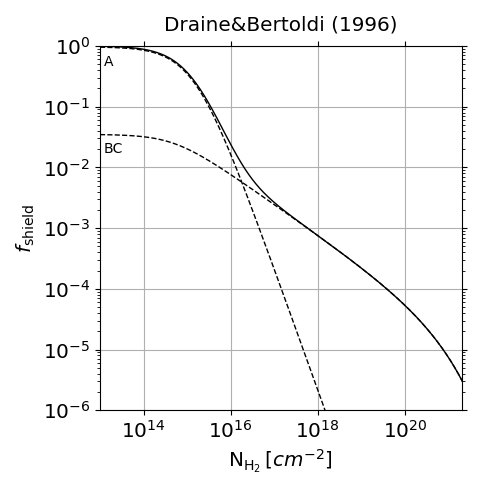
\includegraphics[width = 0.4\textwidth]{figure/H2/pumpingH2/fshield.png}
%     \caption{Fonction de shielding $f_\mathrm{shield}$ de $\mathrm{H}_2$ en fonction de la colonne densité $N(\mathrm{H}_2)$}
%     \label{fig:H2:fshield}
% \end{figure}


\subsubsection{Extinction par les grains}

Le champs de rayonnement calculé par le code ne prend pas en compte l'extinction par les grains. Approximation FGK. Je corrige le champs de rayonnement par $e^{-\tau_d}$ où $\tau_d = N_\mathrm{H}\sigma_d$ donné par \cite{SternbergLePetit2014} Eq 20. Ainsi, 

$$\chi^{'} = e^{-\tau_d
}\, f_{\mathrm{shield}}\, \chi$$


\subsubsection{Comparaison avec le code PDR de Meudon}

On récupère du code le taux de refroidissement $\Lambda_{\mathrm{PDR}}$ par la molécule $\mathrm{H}_2$ qui peut être positif ou négatif. Le taux prend en compte du chauffage par desexcitation collisionnelle et du refroidissement ro-vibrationelle (émission). Il ne prend pas en compte de la photodissociation (qui chauffe). On veut étudier le chauffage, on appelle $\Gamma_{\mathrm{PDR}}$ la partie négative du taux ($\Lambda_{\mathrm{PDR}} < 0$) et on le compare aux de chauffage nets.

\begin{equation}
    \begin{split}
        \Gamma_{\mathrm{Rollig} \, \mathrm{net}} &= \Gamma_{\mathrm{H}_2^\star} + \Lambda_{\mathrm{H}_2} \\ 
        \Gamma_{\mathrm{BS} \, \mathrm{net}} &=\Gamma_{\mathrm{H}_2 \, \mathrm{pump}} +  \Gamma_{\mathrm{H}_2 \, \mathrm{pd}} 
    \end{split}
\end{equation}

La figure \ref{fig:H2:GammaPDR} compare les taux de chauffages nets utilisant différentes prescriptions à celui calculé dans le code (en noir). Le chauffage calculé par Rollïg et de Bialy\&Sternberg ont la même intensité en bord de nuage où la désexcitation collisionnelle est prédominante. 

L'approximation FGK est une méthode qui calcule le spectre du champs de rayonnements à travers le nuage qui prend en compte l'absorption dans le continuum et le carbone. Il prend également en compte l'écrantage de la molécule $\mathrm{H}_2$ (figure \ref{fig:H2:fgk} \cite{FGK}). 

% \begin{figure}[h!]
%     \centering
%     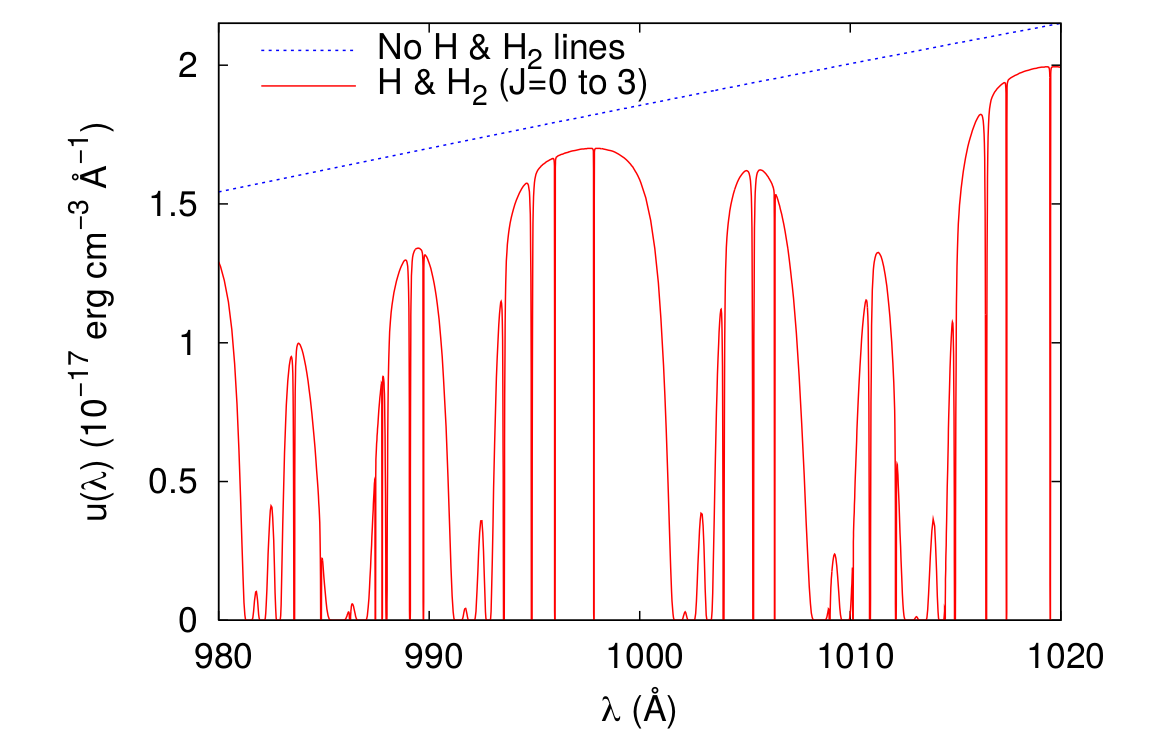
\includegraphics[width = 0.6\textwidth]{figure/H2/fgk.png}
%     \caption{Densité d'énergie au sein d'un nuage à un $A_\mathrm{V}=0.5$. Les niveaux du $\mathrm{H}$ et de $\mathrm{H}_2$ absorbent certains photons sur certaines raies. A mesure que l'on s'enfonce dans le nuage beaucoup de matière se trouve sur la ligne de visée et les raies d'absroptions s'élargissent (voir optiquement épaisse Draine) \cite{FGK}}
%     \label{fig:H2:fgk}
% \end{figure}

%%%%%%%%%%%%%%%%%%%%%%%%%%%%%%%%%%%%%%%%%%%%%%%%%%%%%%%%%%%%%%%%%%%%%%%%%%%%%

\subsection{Dissociation collisionelle du $\mathrm{H}_2$ (de Janev à Glover)}

La destruction du $\mathrm{H}_2$ dans les nuages interstellaire s'effectue soit par photodissociation soit par réactions chimiques. Les dissociations collisionnelles (eq. \ref{eq:H2diss}) sont des réactions de destruction du $\mathrm{H}_2$ mal connues alors qu'elles interviennent dans du gaz chaud, ce qui est le cas du bord atomique de la PDR jusqu'à la transition $\mathrm{H}/\mathrm{H}_2$. 

\begin{equation}\label{eq:H2diss}
    \begin{array}{lcccccccl}
        \mathrm{H} & + & \mathrm{H}_2   & \rightarrow &\mathrm{H}  & + & \mathrm{H} & + & \mathrm{H} \\
        \mathrm{H}_2  & + & \mathrm{H}_2  & \rightarrow & \mathrm{H} & + &\mathrm{H}_2  & + & \mathrm{H} \\
    \end{array}
\end{equation}

Il existe plusieurs prescriptions qui tentent d'estimer les valeurs des taux de dissociation collisionelle du $\mathrm{H}_2$ (eq \ref{eq:H2diss}) en fonction de la température et des niveaux de la molécule. Connaître leurs taux de réaction est important car ils changent la densité de $\mathrm{H}_2$ à travers le nuage ce qui a un impact sur le chauffage par $\mathrm{H}_2$ et donc la température du gaz. Deux prescriptions possibles ont été retenu dans le code : celle de Glover et Mac Low (article) et celle de Janev (article). Par ailleurs on a constaté que la prescription de Glover calcule des taux de dissociation très faible (d'un facteur $10^{-50}$ bof) devant ceux de Janev ce qui change radicalement la chimie du nuage. Afin de n'en garder qu'une, nous avons comparé les effets de ces prescriptions sur l'ensemble des PDR. \newline 

Pour étudier globalement les PDR, on utilise des grilles de modèles qui explorent l'espace des paramètres (pression $\mathrm{P}$, densité $n_\mathrm{H}$ et le champ de rayonnement de l'étoile proche $\chi$). On représente une donnée - la température au bord de nuage, la température et l'$\mathrm{A}_\mathrm{v}$ de la transition $\mathrm{H}/\mathrm{H}_2$ ou le processus thermique dominant au bord du nuage - à travers la grille et étudions quelques modèles particuliers afin de comprendre profondément les changements sur le code. On étudie d'abord des modèles à densités constantes qui sont plus facile à interpréter (la pression et la température suivent les mêmes variations $\mathrm{P}\propto \mathrm{T}$) que les modèles isobares (la densité et la température varient de manière inversement proportionelle $\mathrm{n}_\mathrm{H}\mathrm{T}=\mathrm{cte}$).    

\subsubsection{Grilles de modèles - Bord atomique}

Sur la figure \ref{fig:H2:JanevGlover:Tba}, la température en bord de nuage atomique est représentée. On constate qu'elle est sensiblement similaire selon que l'on utilise la prescription de Janev ou de Glover à l'exception des PDR denses et fortement illuminées ($n_\mathrm{H} \geq 10^{4.5} \, \mathrm{cm}^{-3}$ et $\chi \geq 10^3$) qui sont légèrement plus chaudes. En visualisant sur la figure \ref{fig:H2:JanevGlover:diffTba} la différence des cartes de température, on comprend que la prescription de Glover a tendance à chauffer les bords atomiques de l'ensemble des PDR de $+200$ K et peut augmenter la température jusqu'à $+800$ K pour les PDR denses et fortement illuminées. \newline


\begin{figure}[!h]
    \centering
    \begin{subfigure}[t]{0.49\textwidth} % "0.49" donne ici la largeur de l'image
        \centering 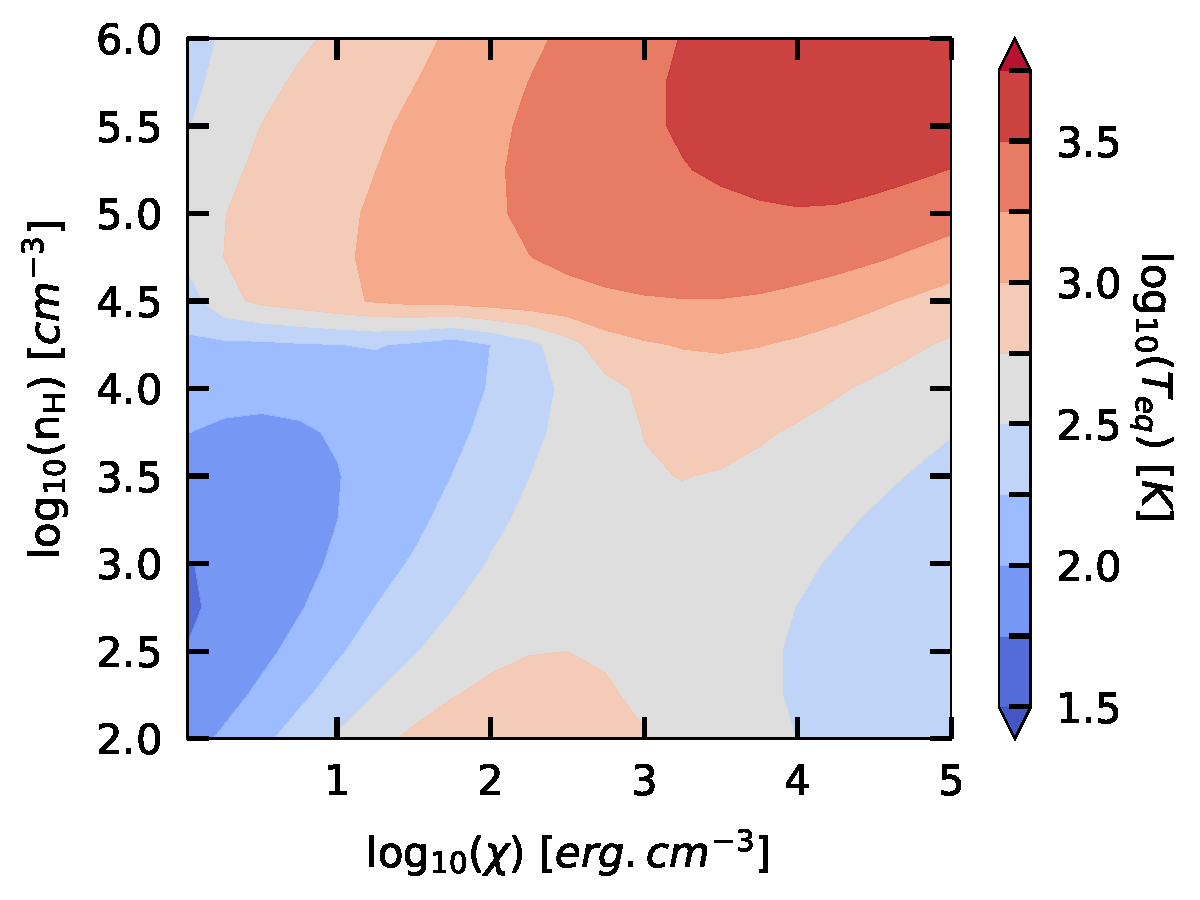
\includegraphics[trim = {0 0 0 0 },clip,width=1\textwidth]{figure/H2/grid_janev/mapTba.pdf}
        \caption{Janev}
    \end{subfigure}
    ~ 
    \begin{subfigure}[t]{0.49\textwidth}
        \centering 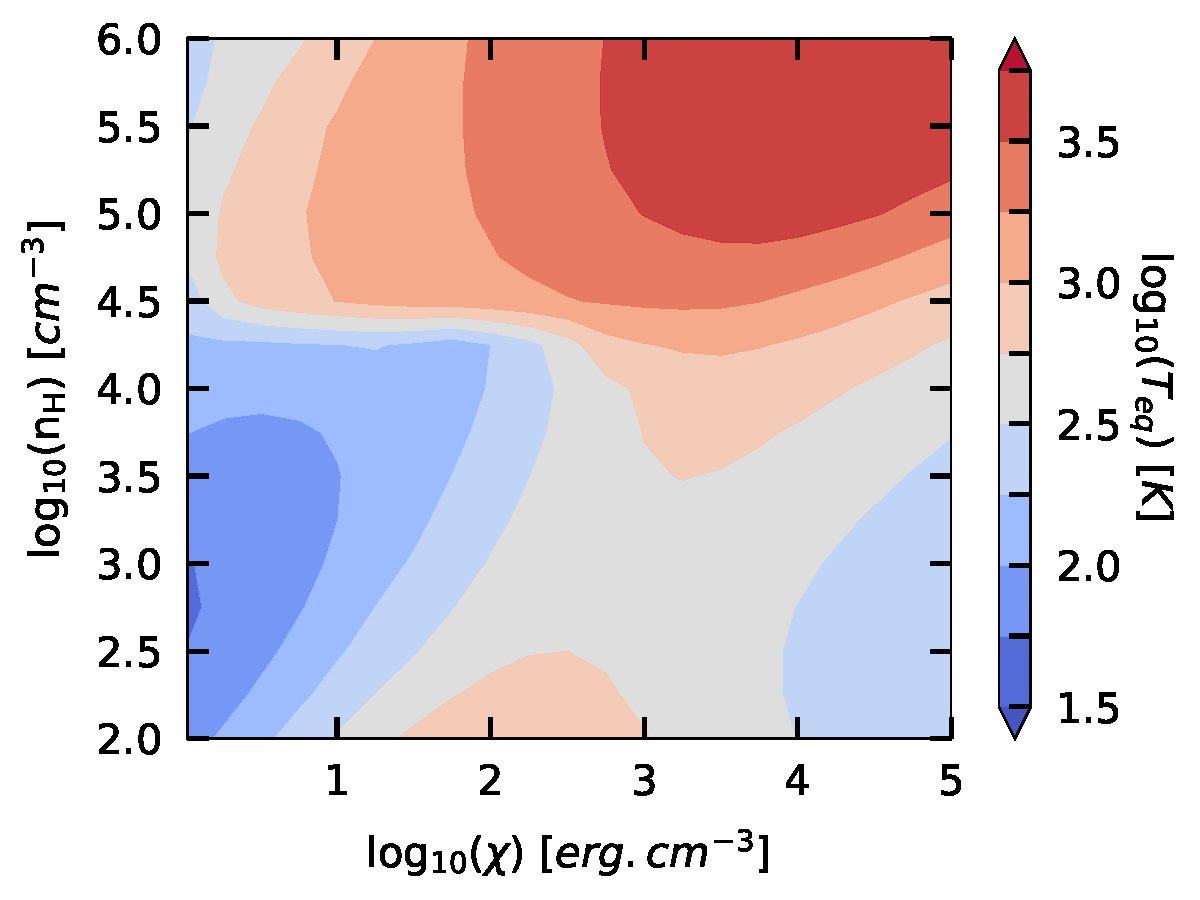
\includegraphics[trim = {0 0 0 0 },clip,width=1\textwidth]{figure/H2/grid_glover/mapTba.pdf}
        \caption{Glover}
    \end{subfigure}
    \caption{Comparaison des température en bord atomique de nuage pour des modèles utilisant la prescription de Janev et de Glover}
    \label{fig:H2:JanevGlover:Tba}
\end{figure}


Cette différence est principalement due à l'amélioration du chauffage par pompage UV de la molécule $\mathrm{H}_2$. Il devient en effet plus efficace de former du $\mathrm{H}_2$ dans les bords atomiques des nuages grâce taux calculés par Glover. Le chauffage par pompage UV étant d'autant plus efficace que la densité de $\mathrm{H}_2$ est grande, les bords atomiques de l'ensemble des PDR sont plus chauds. Le pompage UV devient encore plus intense dans les PDR denses et fortement illuminés où la densité de molécule $\mathrm{H}_2$ et la quantité de photons UV deviennent importantes (hum le refroidissement par les raies également nan ?). \newline

On constate sur la figure \ref{fig:H2:JanevGlover:Gmax} que le chauffage par $\mathrm{H}_2$ reste dominant dans les bords atomique des PDR denses quelque soit la prescription que l'on utilise. En revanche, les processus de refroidissements (figure \ref{fig:H2:JanevGlover:Lmax}) varient pour les PDR denses et faiblement illuminées ($n_\mathrm{H} \geq 10^{4.5} \, \mathrm{cm}^{-3}$ et $\chi \leq 10^3$). L'utilisation des taux de dissociation de Glover tue le refroidissement par les réactions chimiques ce qui est normal car les réactions de dissociation du $\mathrm{H}_2$ (eq \ref{eq:H2diss}) sont des réactions endothermiques très efficaces.

\begin{figure}[!h]
    \centering
    \begin{subfigure}[t]{0.49\textwidth} % "0.49" donne ici la largeur de l'image
        \centering 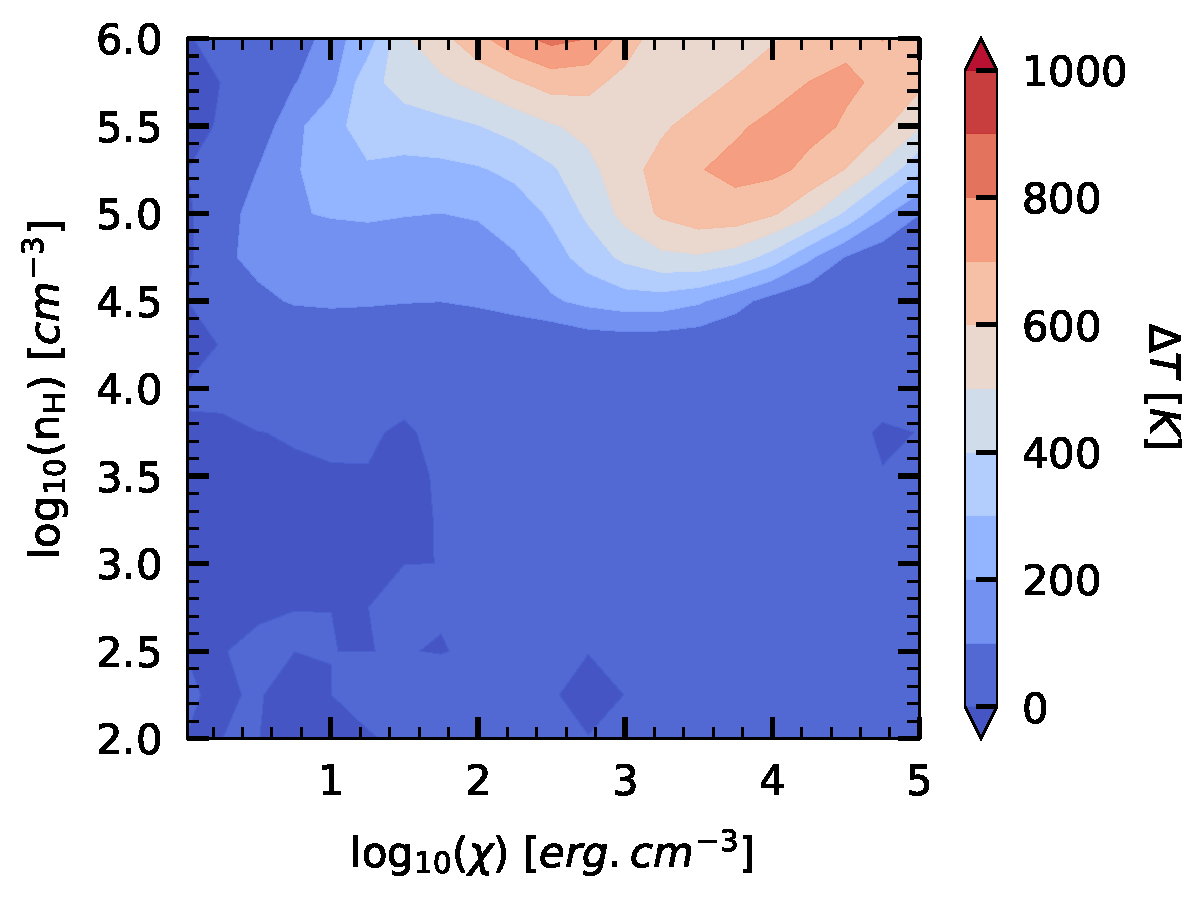
\includegraphics[trim = {0 0 0 0 },clip,width=1\textwidth]{figure/H2/diffgrid_gloverjanev/mapTba_H2_n_1p7_nobossion_noCl155_n.pdf}
        \caption{Différence de température au bord}
        \label{fig:H2:JanevGlover:diffTba}
    \end{subfigure}
    ~ 
    \begin{subfigure}[t]{0.49\textwidth}
        \centering 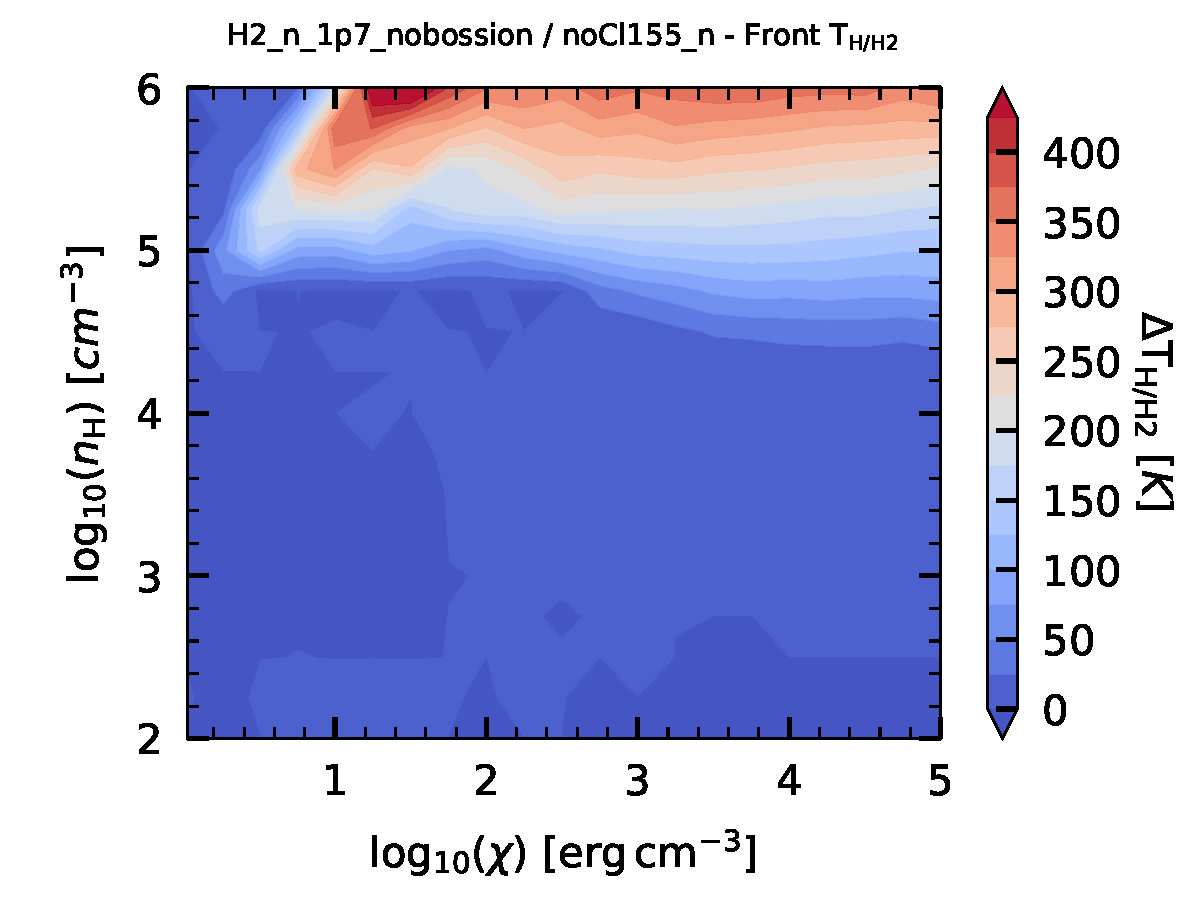
\includegraphics[trim = {0 0 0 1cm },clip,width=1\textwidth]{figure/H2/diffgrid_gloverjanev/HH2_T_H2_n_1p7_nobossion_noCl155_n.pdf}
        \label{fig:H2:JanevGlover:diffTmax}
        \caption{Différence de température à la transition $\mathrm{H}/\mathrm{H2}$}
        \label{fig:H2:JanevGlover:diffTHH2}
    \end{subfigure}
    \caption{Différence de température aux bords de nuage et aux transitions $\mathrm{H}/\mathrm{H}_2$ de modèles utilisant la prescription de Janev et de Glover (les cartes ne sont pas en harmonie)}
\end{figure}

\begin{figure}[!h]
    \centering
    \begin{subfigure}[t]{0.49\textwidth} % "0.49" donne ici la largeur de l'image
        \centering 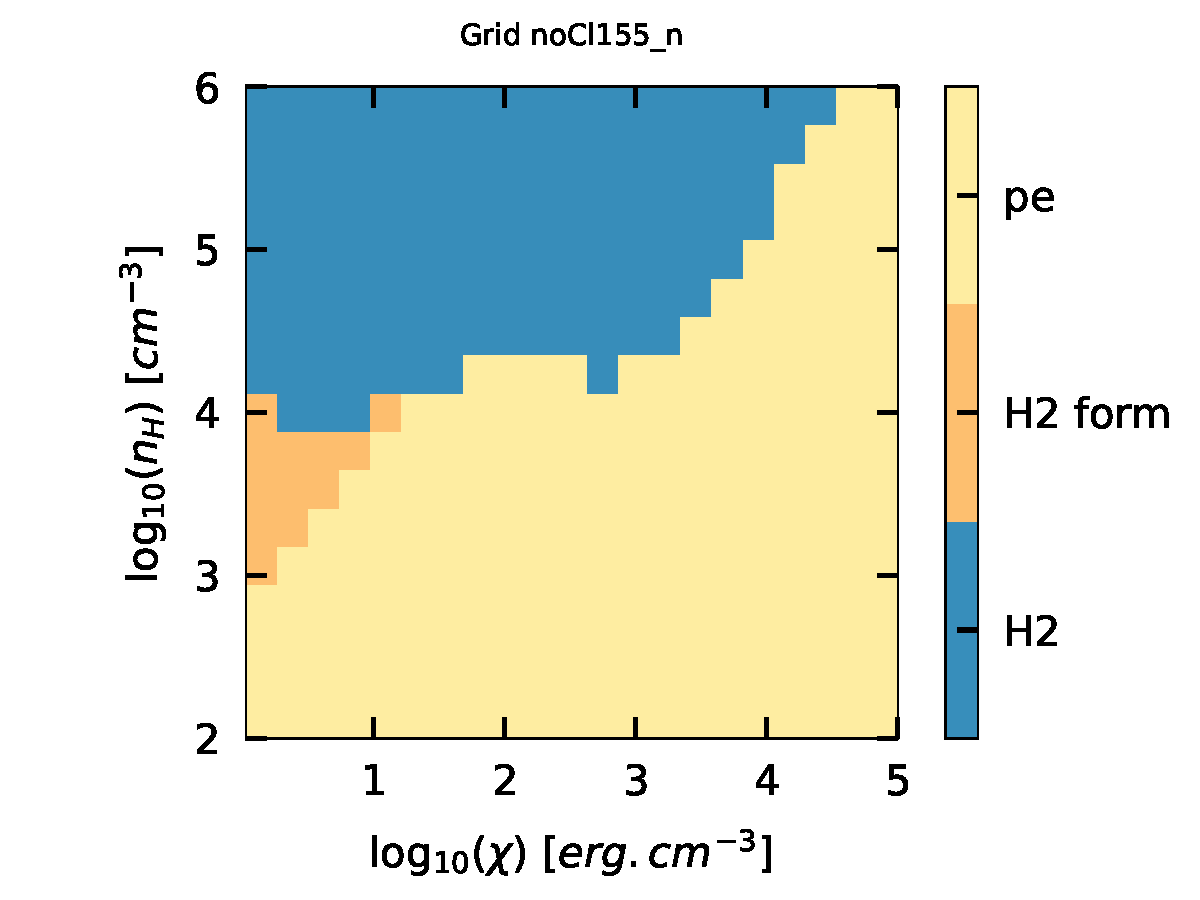
\includegraphics[trim = {0 0 0 1cm },clip,width=1\textwidth]{figure/H2/grid_janev/mapGmax.pdf}
        \caption{Janev}
    \end{subfigure}
    ~ 
    \begin{subfigure}[t]{0.49\textwidth}
        \centering 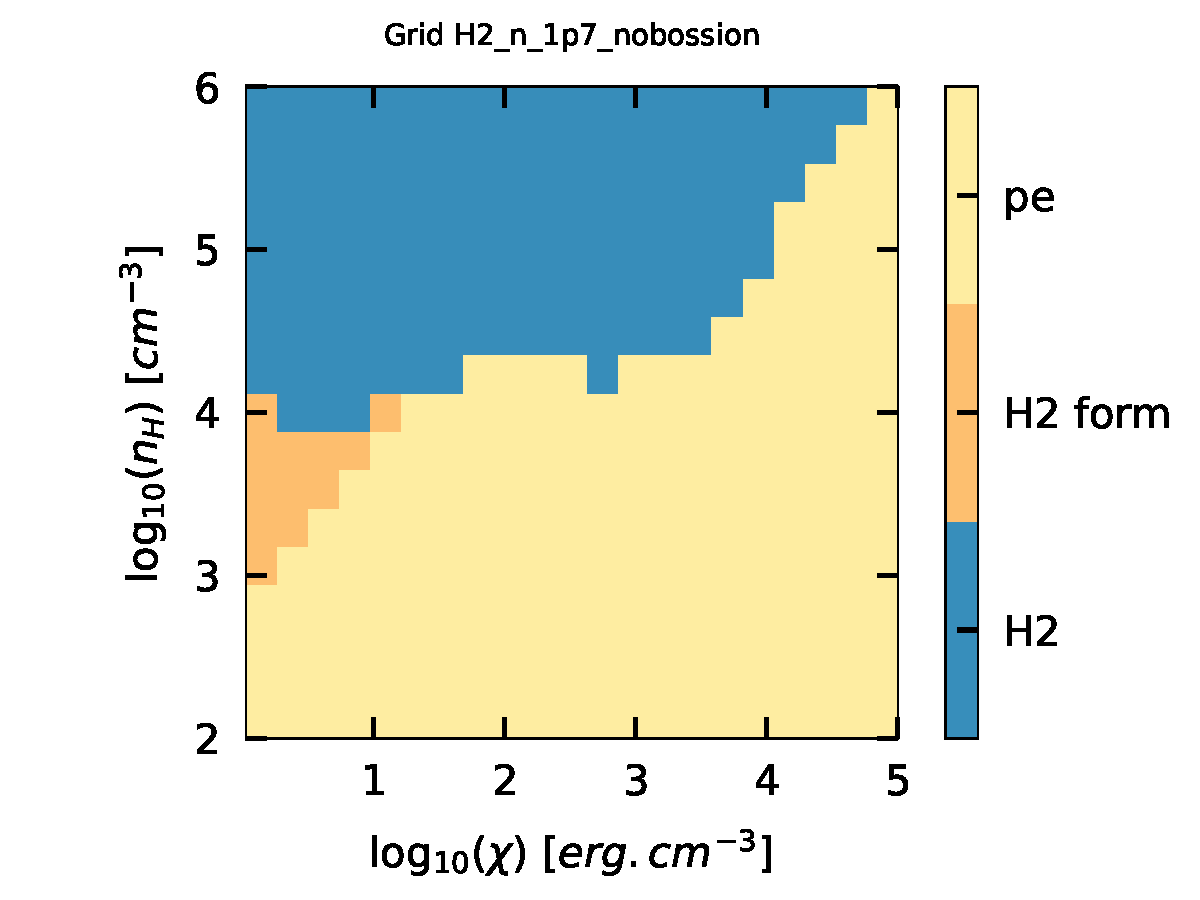
\includegraphics[trim = {0 0 0 1cm },clip,width=1\textwidth]{figure/H2/grid_glover/mapGmax.pdf}
        \caption{Glover}
    \end{subfigure}
    \caption{Processus de chauffage dominant en bord de région atomique}
    \begin{minipage}{\textwidth}
    Le chauffage par effet photoélectrique sur les grains est désigné ici sous l'abréviation "pe". "H2" désigne le chauffage par pompage UV de la molécule $\mathrm{H}_2$ et "H2 form" la formation de la molécule sur les grains.
    \end{minipage}
    \label{fig:H2:JanevGlover:Gmax}
    \hspace{1em}
    
    \begin{subfigure}[t]{0.49\textwidth} % "0.49" donne ici la largeur de l'image
        \centering 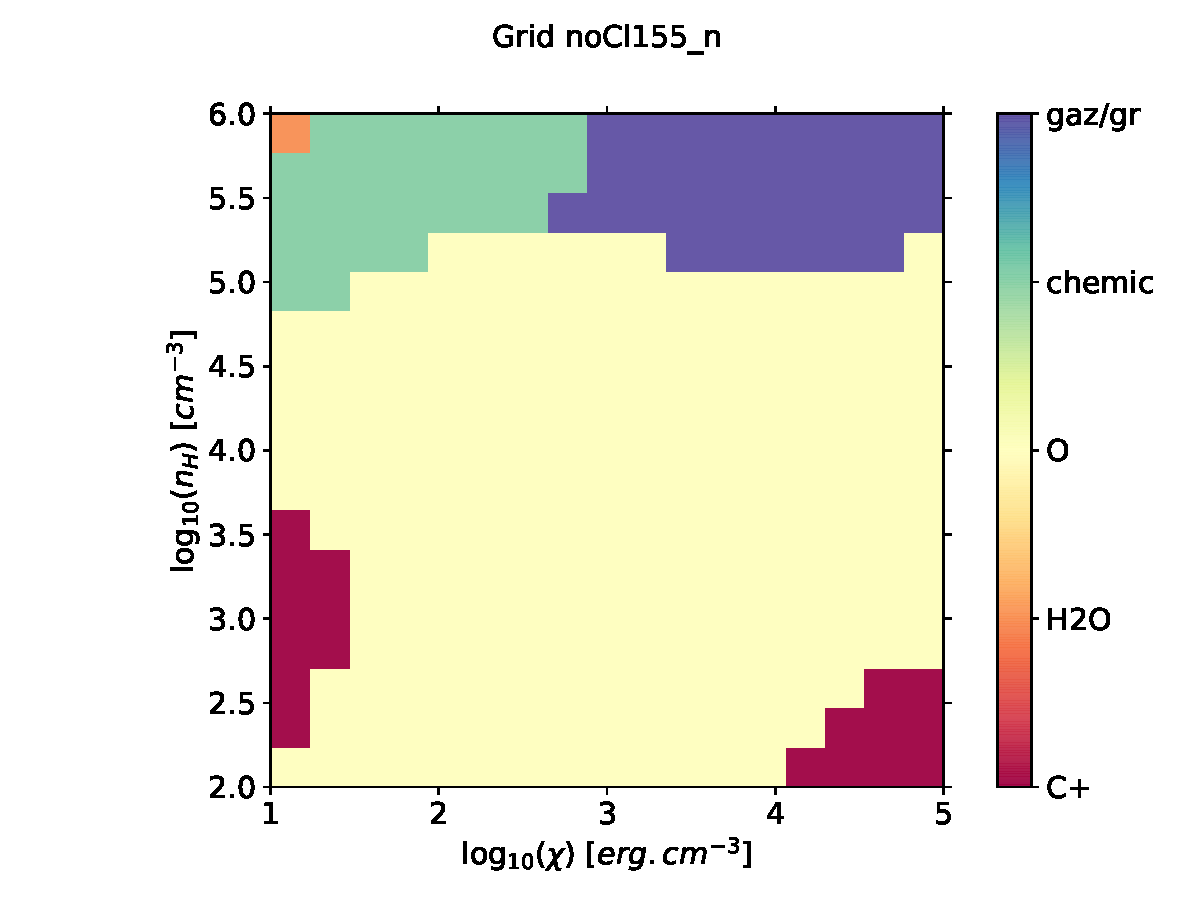
\includegraphics[trim = {0 0 0 1cm },clip,width=1\textwidth]{figure/H2/grid_janev/mapLmax.pdf}
        \caption{Janev}
    \end{subfigure}
    ~ 
    \begin{subfigure}[t]{0.49\textwidth}
        \centering 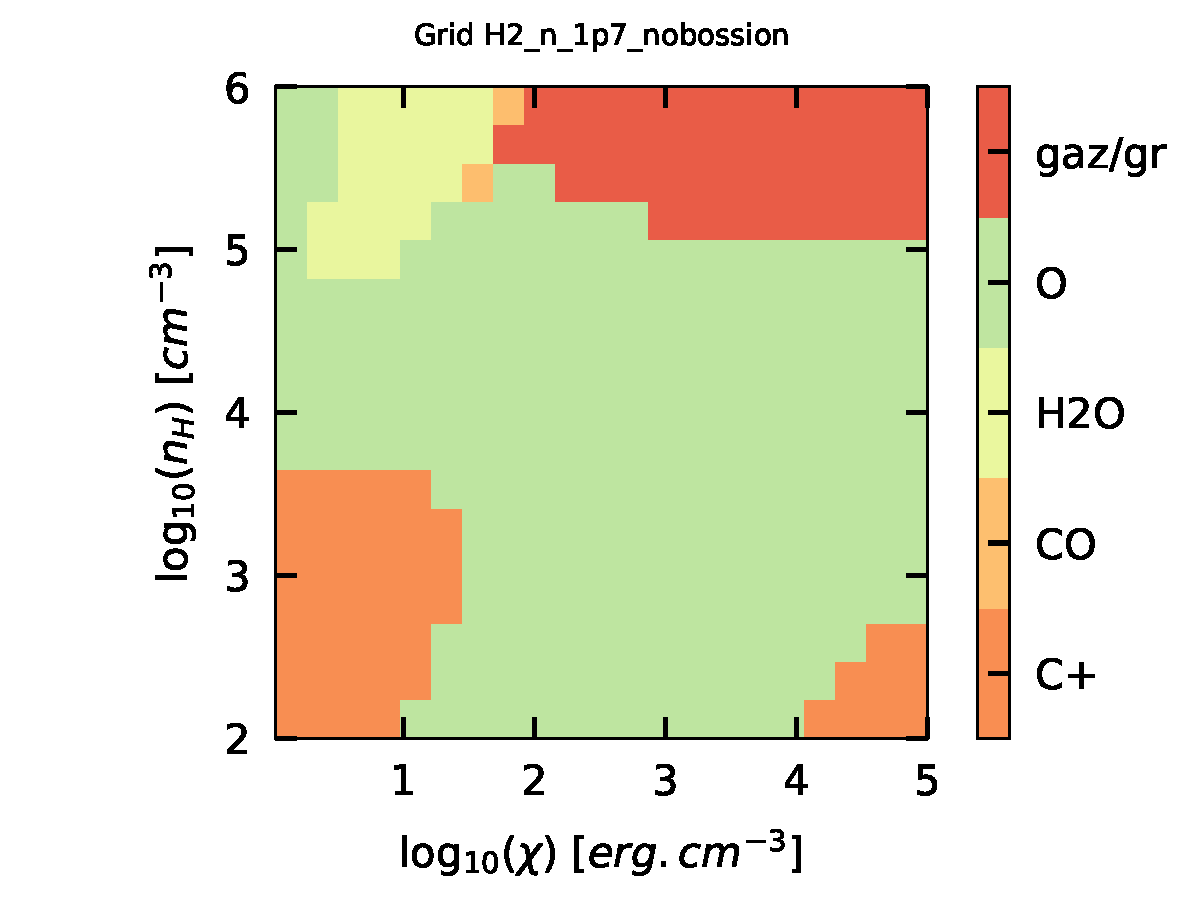
\includegraphics[trim = {0 0 0 1cm },clip,width=1\textwidth]{figure/H2/grid_glover/mapLmax.pdf}
        \caption{Glover}
    \end{subfigure}
    \caption{Processus de refroidissement dominant en bord de région atomique}
    \begin{minipage}{\textwidth}
    Les noms "O", "H2O", "CO" et "C+" désignent des processus de refroidissement par désexcitation collisionelles des espèces $\mathrm{O}$, $\mathrm{H}_2\mathrm{O}$, $\mathrm{CO}$ et $\mathrm{C}^+$ respectivement. "gaz/gr" réfère à la thermalisation du gaz avec les grains du nuage généralement plus froid ($\mathrm{T}\sim20$ K) et "chemic" au bilan thermique des réactions chimiques qui est ici endothermique.
    \end{minipage}
    \label{fig:H2:JanevGlover:Lmax}
\end{figure}


%%%%%%%%%%%%%%%%%%%%%%%%%%%%%%%%%%%%%%%%%%%%%%%%%%%%%%%%%%%%%%%%%%%%%%%%%%%%%%
\subsubsection{Grilles de modèles - Transition $\mathrm{H}/\mathrm{H}_2$}

La transition $\mathrm{H}/\mathrm{H}_2$ marque la frontière entre le milieu atomique et moléculaire du nuage. Elle survient une fois que le $\mathrm{H}_2$, jusqu'à là détruit dans la zone atomique par les photons UV, parvient à se former en suffisamment grande quantité pour que l'hydrogène soit majoritairement sous forme moléculaire. Nous avons définit le critère tel qu'il y ait autant d'élément hydrogène sous forme atomique que moléculaire soit $n(\mathrm{H}) = 2 n(\mathrm{H}_2)$. La température et l'$\mathrm{A}_\mathrm{v}$ auxquelles s'effectuent la transition $\mathrm{H}/\mathrm{H}_2$ ont un impact sur les observables puisque que c'est dans la phase moléculaire que de nombreux traceurs tels que le $\mathrm{H}_2$,  $\mathrm{CO}$, $\mathrm{H}_2\mathrm{O}$ ou $\mathrm{HCN}$ se forment et sont excités (par...le H2 excité ou les grains ?). \newline

Les figures \ref{fig:H2:JanevGlover:THH2} et \ref{fig:H2:JanevGlover:AVHH2} montrent les températures et les $\mathrm{A}_\mathrm{v}$ des transitions de chaques modèles. Alors que la position de la transition dans le nuage reste sensiblement identique (figure \ref{fig:H2:JanevGlover:AVHH2}) en passant de la prescription de Janev à celle de Glover, la température dépasse le seuil limite de $600$ K et atteint les $1000$ K (figure \ref{fig:H2:JanevGlover:THH2}).


\begin{figure}[!h]
    \centering
    \begin{subfigure}[t]{0.49\textwidth} % "0.49" donne ici la largeur de l'image
        \centering 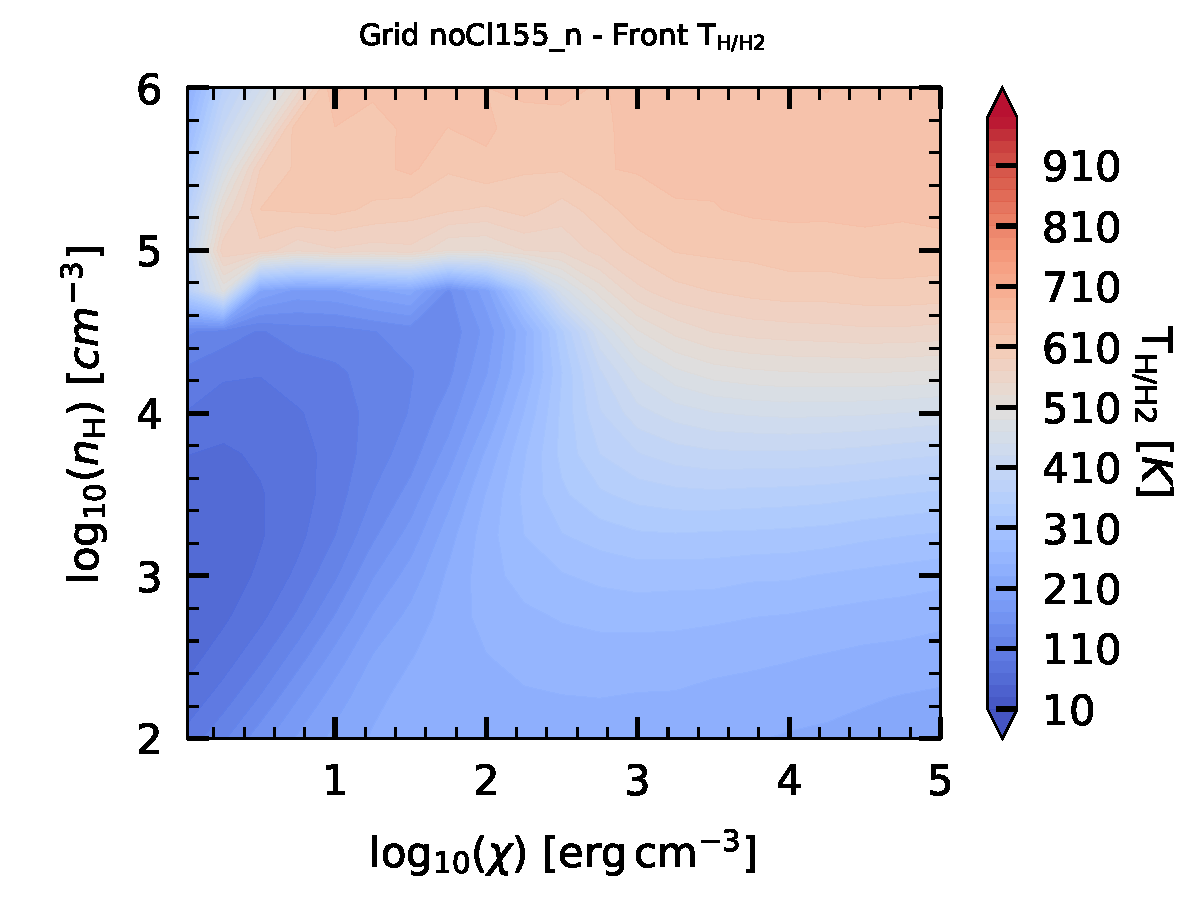
\includegraphics[trim = {0 0 0 1cm },clip,width=1\textwidth]{figure/H2/grid_janev/HH2_T.pdf}
        \caption{Janev}
    \end{subfigure}
    ~ 
    \begin{subfigure}[t]{0.49\textwidth}
        \centering 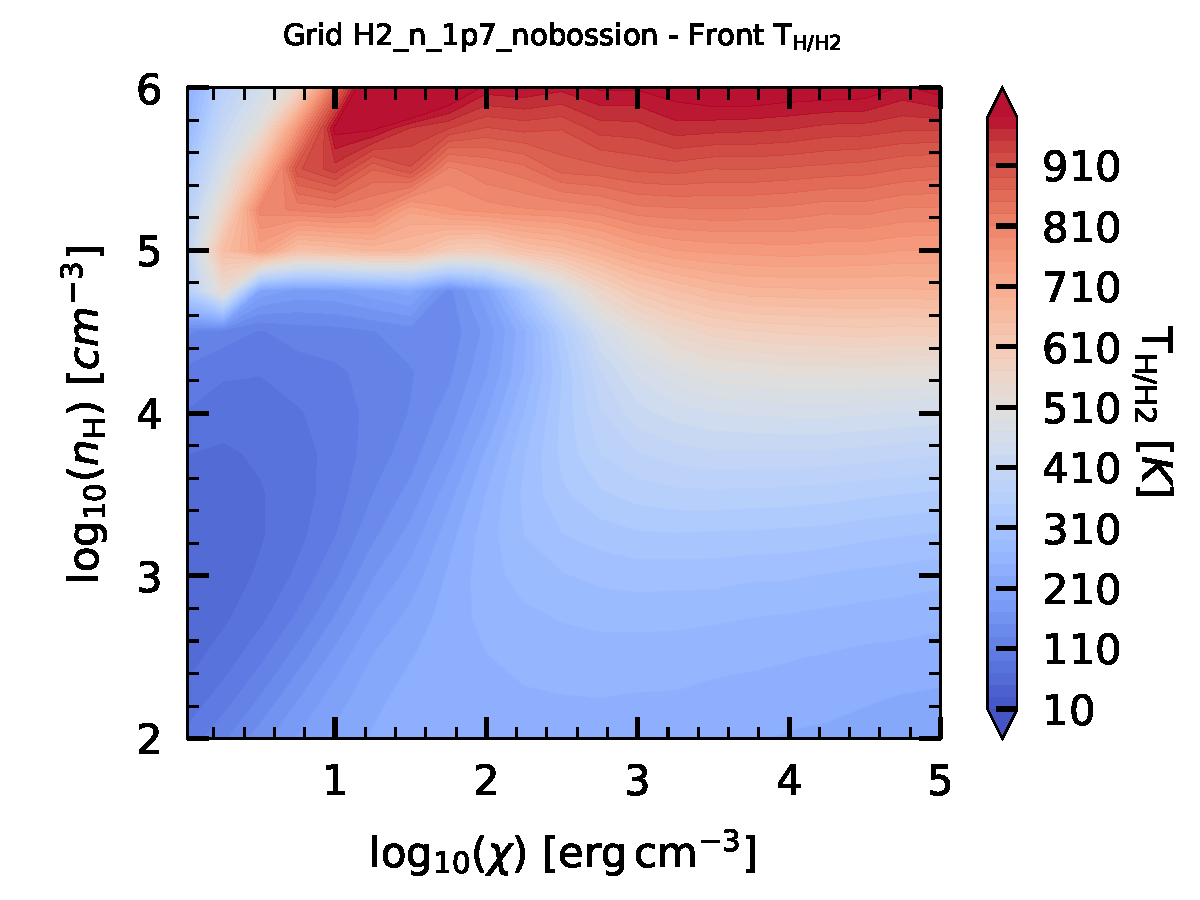
\includegraphics[trim = {0 0 0 1cm },clip,width=1\textwidth]{figure/H2/grid_glover/HH2_T.pdf}
        \caption{Glover}
    \end{subfigure}
    \caption{Comparaison des température à la transition $\mathrm{H}/\mathrm{H}_2$ des modèles utilisant la prescription de Janev et de Glover}
    \label{fig:H2:JanevGlover:THH2}
    
    \centering
    \begin{subfigure}[t]{0.49\textwidth} % "0.49" donne ici la largeur de l'image
        \centering 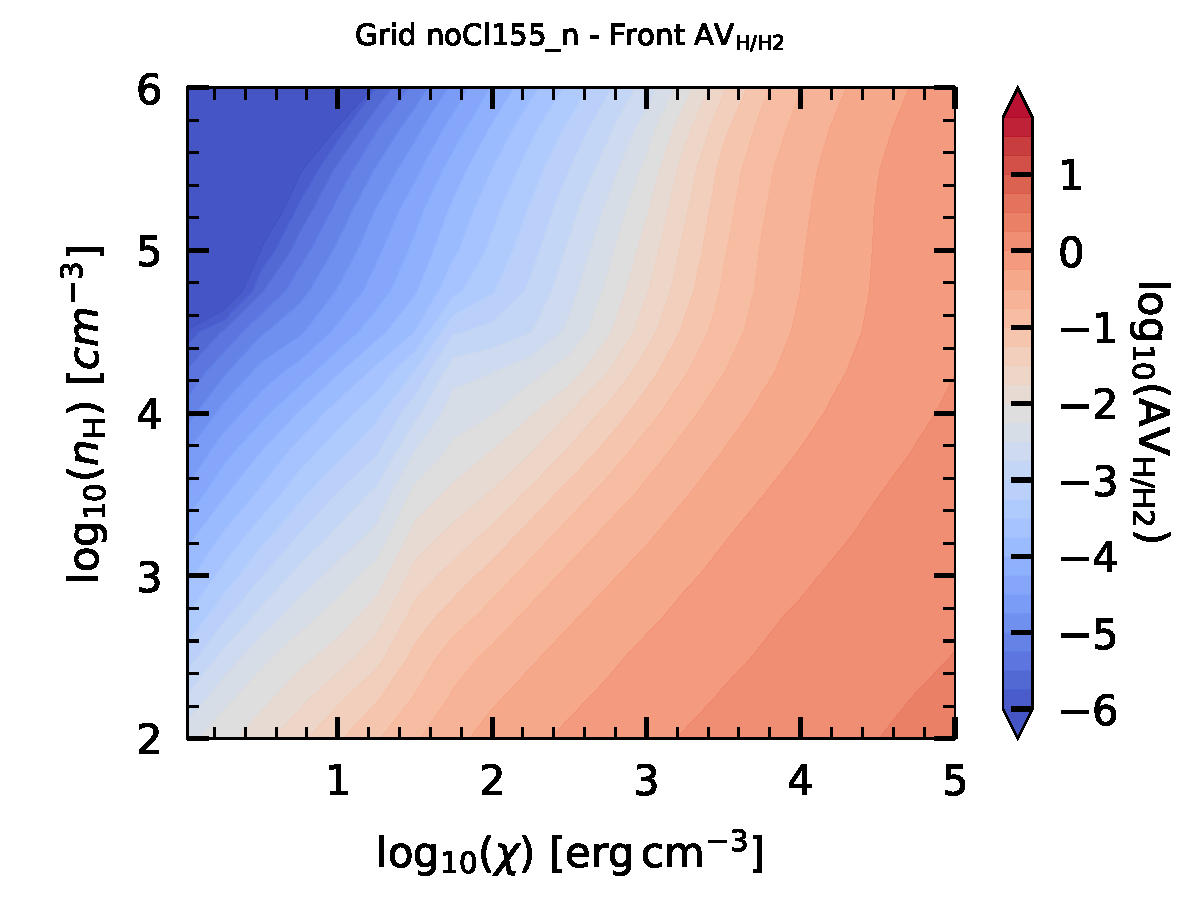
\includegraphics[trim = {0 0 0 1cm },clip,width=1\textwidth]{figure/H2/grid_janev/HH2_AV.pdf}
        \caption{Janev}
    \end{subfigure}
    ~ 
    \begin{subfigure}[t]{0.49\textwidth}
        \centering 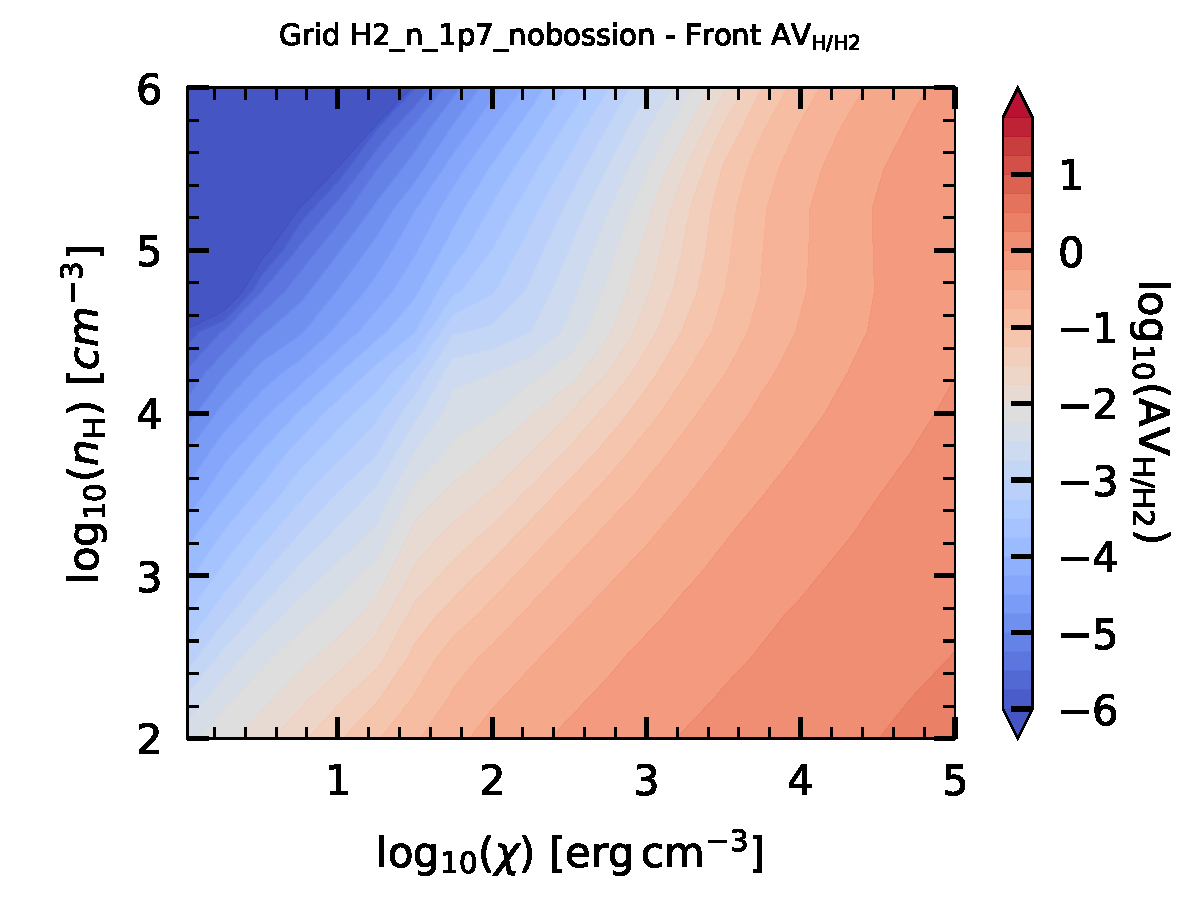
\includegraphics[trim = {0 0 0 1cm },clip,width=1\textwidth]{figure/H2/grid_glover/HH2_AV.pdf}
        \caption{Glover}
    \end{subfigure}
    \caption{Comparaison des $\mathrm{A}_\mathrm{v}$ de la transition $\mathrm{H}/\mathrm{H}_2$ des modèles utilisant la prescription de Janev et de Glover}
    \label{fig:H2:JanevGlover:AVHH2}
\end{figure}
 
 
%%%%%%%%%%%%%%%%%%%%%%%%%%%%%%%%%%%%%%%%%%%%%%%%%%%%%%%%%%%%%%%%%%%%

\subsubsection{Etude d'un modèle particulier}

On cherche à comprendre dans cette section pourquoi la température à la transition $\mathrm{H}/\mathrm{H}_2$ devient plus forte en utilisant la prescription de Glover. On a choisit un modèle à $n_\mathrm{H} = 10^{5.5} \,\mathrm{cm}^{-3}$ et $\chi = 10^4$ qui subit une augmentation de $+300$ K à la frontière. Le profil de température (figure \ref{fig:H2:bosse:plotH}) montre immédiatement une augmentation locale de la température - une bosse - commençant à un $\mathrm{A}_\mathrm{v} \approx 0.1 \,\mathrm{mag}$ et finissant à $\mathrm{A}_\mathrm{v} \approx 0.4 \,\mathrm{mag}$ accompagnée d'une augmentation de la densité de $\mathrm{H}_2$. \newline 

\begin{figure}[!h]
    \centering
    \begin{subfigure}[t]{0.49\textwidth} % "0.49" donne ici la largeur de l'image
        \centering 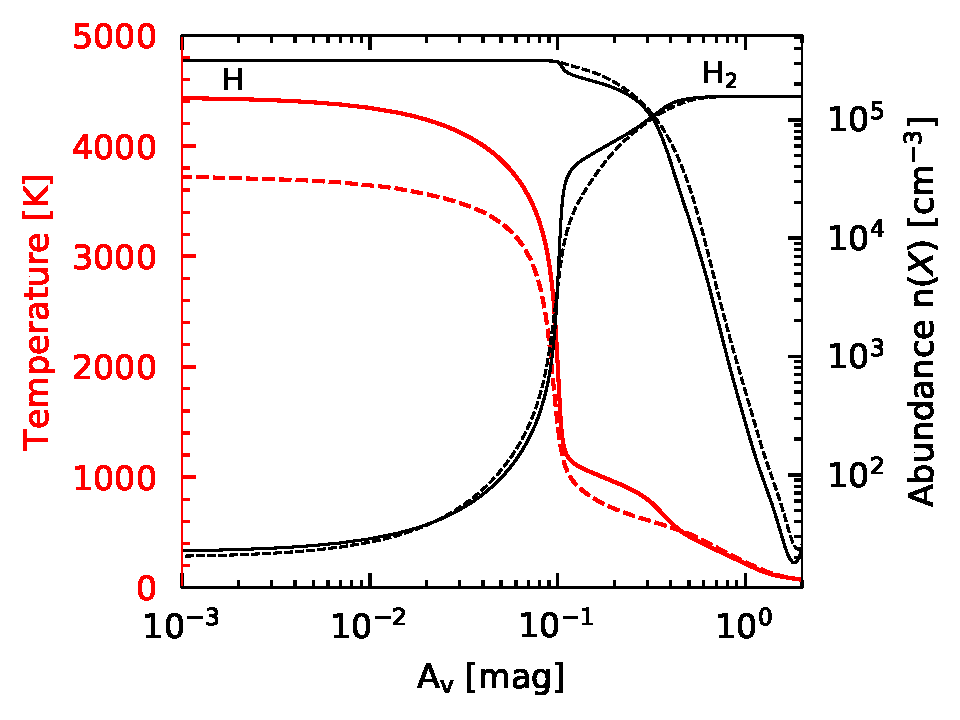
\includegraphics[trim = {0 0 0 0 },clip,width=1\textwidth]{figure/H2/bosse_dcte_janevVSglover/profilT.pdf}
        \caption{}
        \label{fig:H2:bosse:plotH}
    \end{subfigure}
    \begin{subfigure}[t]{0.49\textwidth}
        \centering 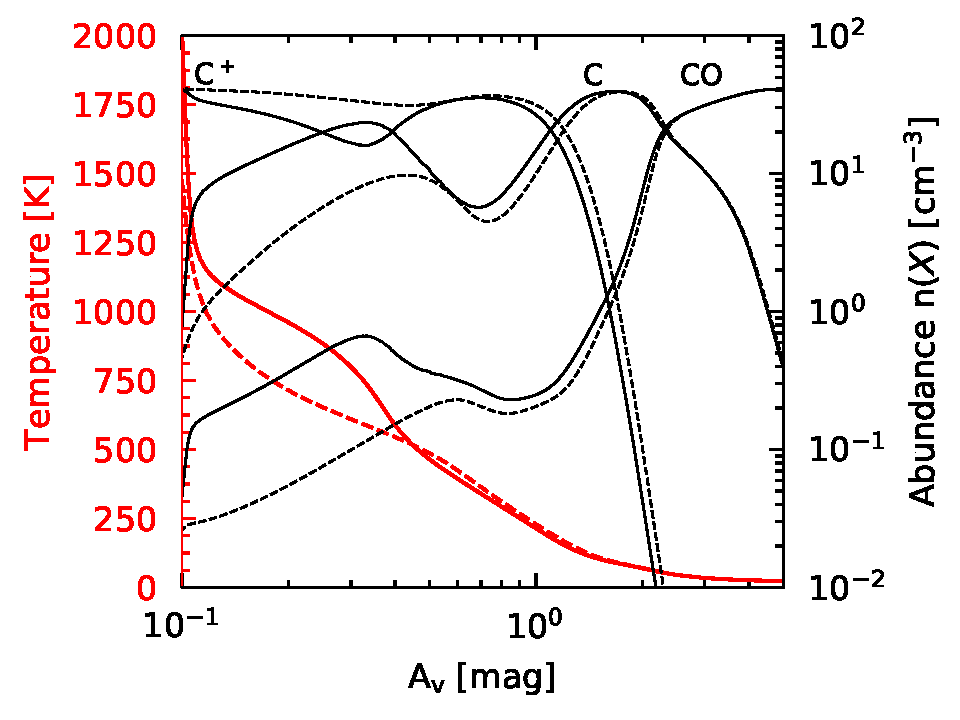
\includegraphics[trim = {0 0 0 0 },clip,width=1\textwidth]{figure/H2/bosse_dcte_janevVSglover/Cp_C_CO.pdf}
        \caption{}
    \label{fig:H2:bosse:plotC}
    \end{subfigure}
    \caption{Profils de densités de $\mathrm{H}$ et $\mathrm{H}_2$ (a) et $\mathrm{C}^+$, $\mathrm{C}$ et $\mathrm{CO}$ (b) d'un modèle à densité constante ($n_\mathrm{H} = 10^{5.5}$ et $\chi = 10^4$). Le trait plein correspond au calcul utilisant la prescription de Glover et les trait pointillés celle de Janev.}
    
\end{figure}

La figure \ref{fig:H2:bosse:heat} trace les taux de chauffages en fonction de l'extinction. On constate, qu'avec la prescription de Glover, les réactions chimiques chauffent le gaz de manière aussi intense que l'effet photoélectrique ce qui peu commun dans les PDR. Afin de comprendre l'origine de la bosse de température, on a tracé à $\mathrm{A}_\mathrm{v} \approx 0.2 \,\mathrm{mag}$, soit au milieu de la bosse, les courbes de chauffages et de refroidissements en fonction de la température (figure \ref{fig:H2:bosse:GC}). L"équilibre thermique du gaz est déterminée par l'intersection de la courbe de chauffage et de refroidissement total. A première vue, les allures des courbes sont très différentes. En passant de la prescription de Janev à celle de Glover, on voit qu'un nouveau processus de chauffage intervient entre $100$ K et $1000$ K. Il s'agit des réactions chimiques qui se mettent à chauffer le gaz de manière plus efficace (figure \ref{fig:H2:bosse:chem}). \newline

Une étude préliminaire montre que la recombinaison électronique du $\mathrm{CH}_3^+$ est la réaction exothermique prédominante dans le chauffage du aux réactions chimiques. Le passage de la prescription de Janev à celle de Glover a pour effet de tuer la destruction du $\mathrm{H}_2$ permettant de rendre le bilan d'exothermicité des réactions chimiques positif et de former plus facilement du $\mathrm{H}_2$ qui va devenir un agent refroidissant efficace. On le visualise simplement sur la figure $\ref{fig:H2:bosse:GC}$. \newline



% L'augmentation de l'intensité des raies se comprend On constate également sur la figure $\ref{fig:H2:bosse:plotC}$ qui représente la transition $\mathrm{C}^+/\mathrm{C}/\mathrm{CO}$ que l. La prescription de Glover permet la formation de $\mathrm{CO}$ chaud 



\begin{figure}[!h]
    \centering
    \begin{subfigure}[t]{0.49\textwidth} % "0.49" donne ici la largeur de l'image
        \centering 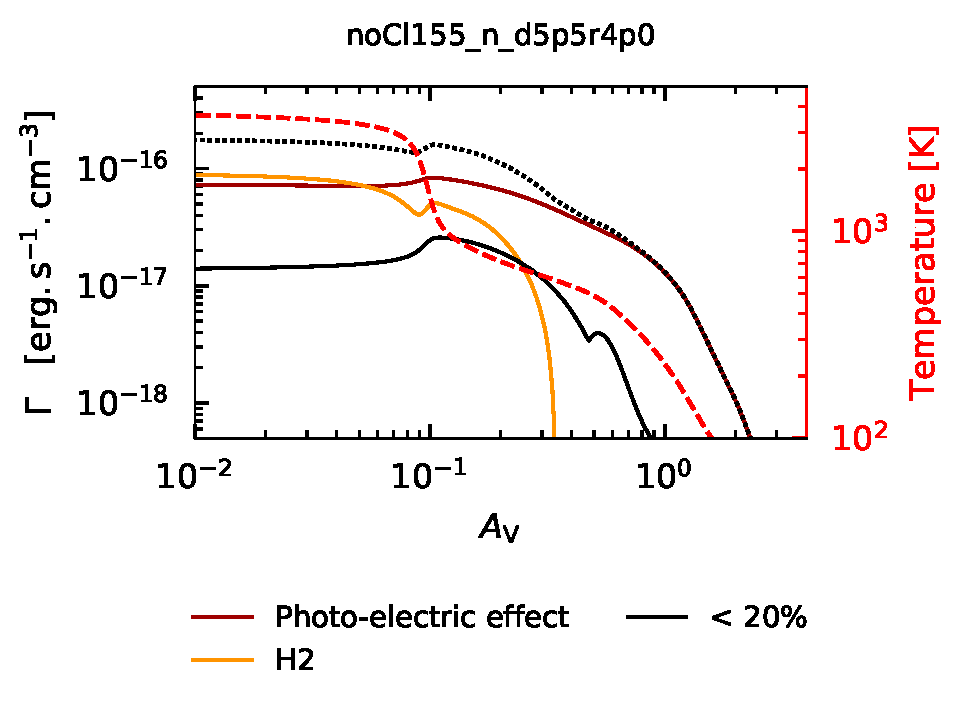
\includegraphics[trim = {0 0 0 1cm },clip,width=1\textwidth]{figure/H2/bosse_dcte_janevVSglover/janev/heat.pdf}
        \caption{Janev}
    \end{subfigure}
    \begin{subfigure}[t]{0.49\textwidth}
        \centering 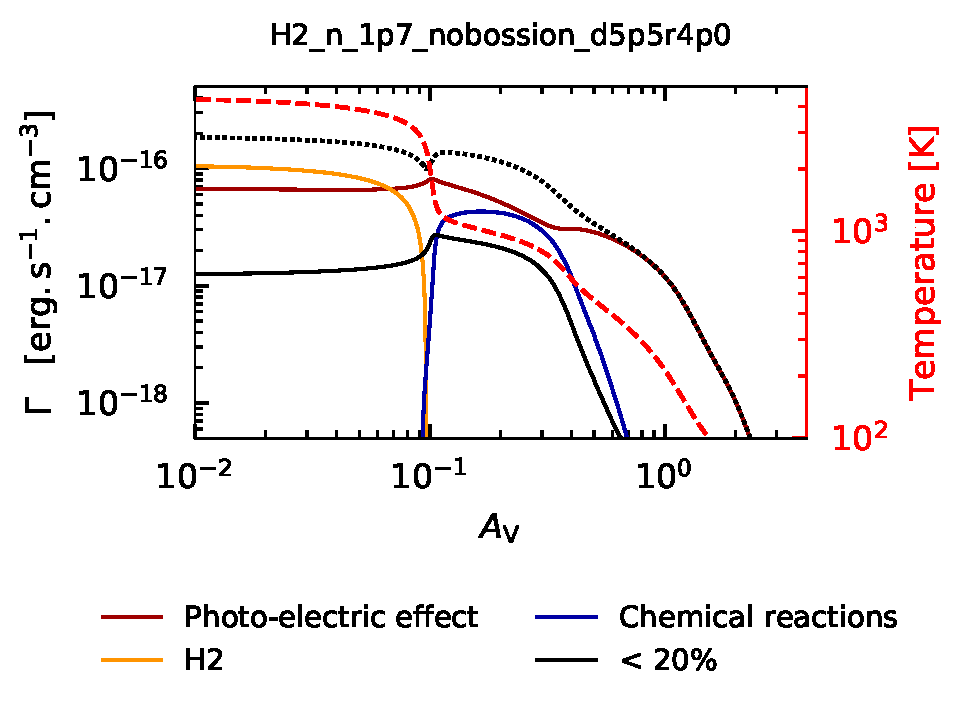
\includegraphics[trim = {0 0 0 1cm },clip,width=1\textwidth]{figure/H2/bosse_dcte_janevVSglover/glover/heat.pdf}
        \caption{Glover}
    \end{subfigure}
    \caption{(ANNEXE) Profils des taux de chauffages d'un modèle à densité constante ($n_\mathrm{H} = 10^{5.5}$ et $\chi = 10^4$) utilisant la prescription de Janev ou de Glover. La température (axe de droite) est représentée en tiret rouge. Le taux de chauffage total est en pointillé noir.}
    \label{fig:H2:bosse:heat}
\end{figure}


\begin{figure}[!h]
    \centering
    \begin{subfigure}[t]{0.49\textwidth} % "0.49" donne ici la largeur de l'image
        \centering 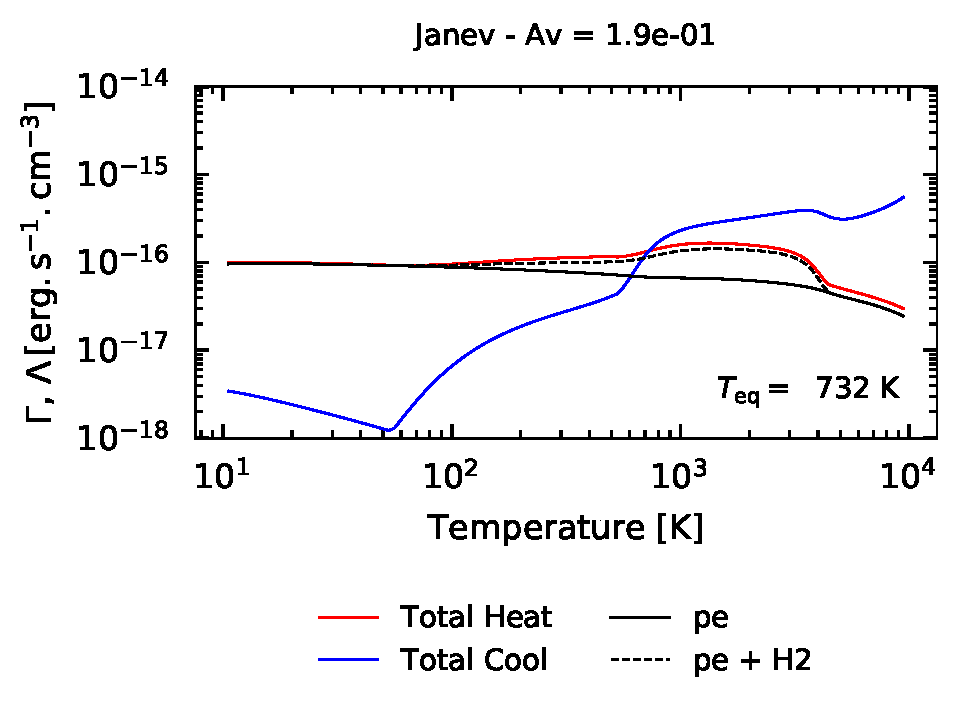
\includegraphics[trim = {0 0 0 1cm },clip,width=1\textwidth]{figure/H2/bosse_dcte_janevVSglover/janev/GC_h_1p9em01.pdf}
        \caption{Janev}
    \end{subfigure}
    \begin{subfigure}[t]{0.49\textwidth}
        \centering 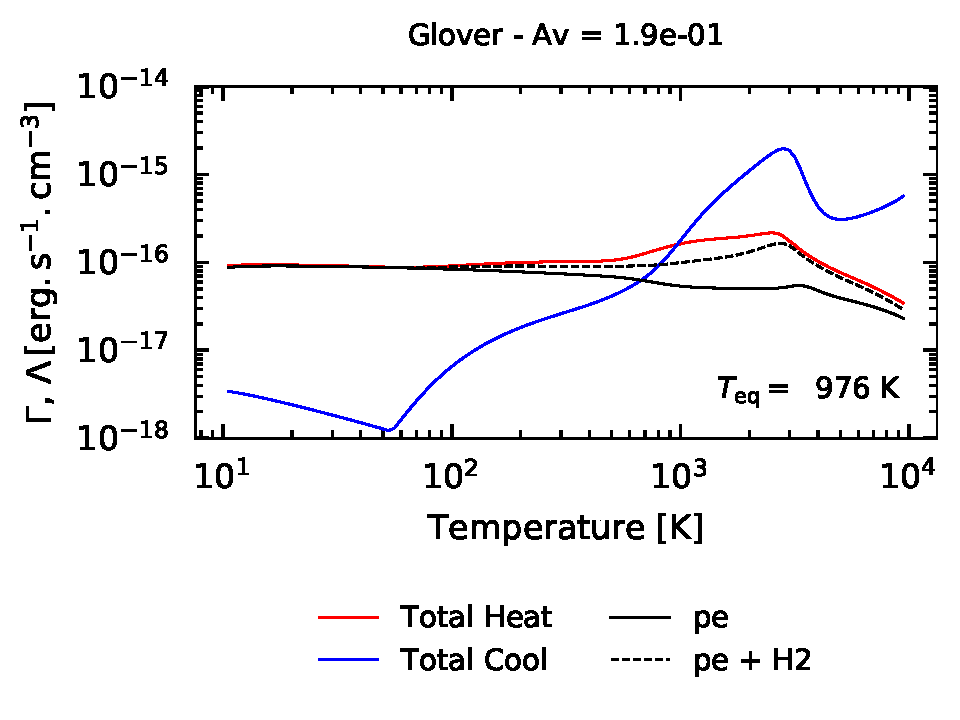
\includegraphics[trim = {0 0 0 1cm },clip,width=1\textwidth]{figure/H2/bosse_dcte_janevVSglover/glover/GC_h_1p9em01.pdf}
        \caption{Glover}
    \end{subfigure}
    ~
    \begin{subfigure}[t]{0.49\textwidth} % "0.49" donne ici la largeur de l'image
        \centering 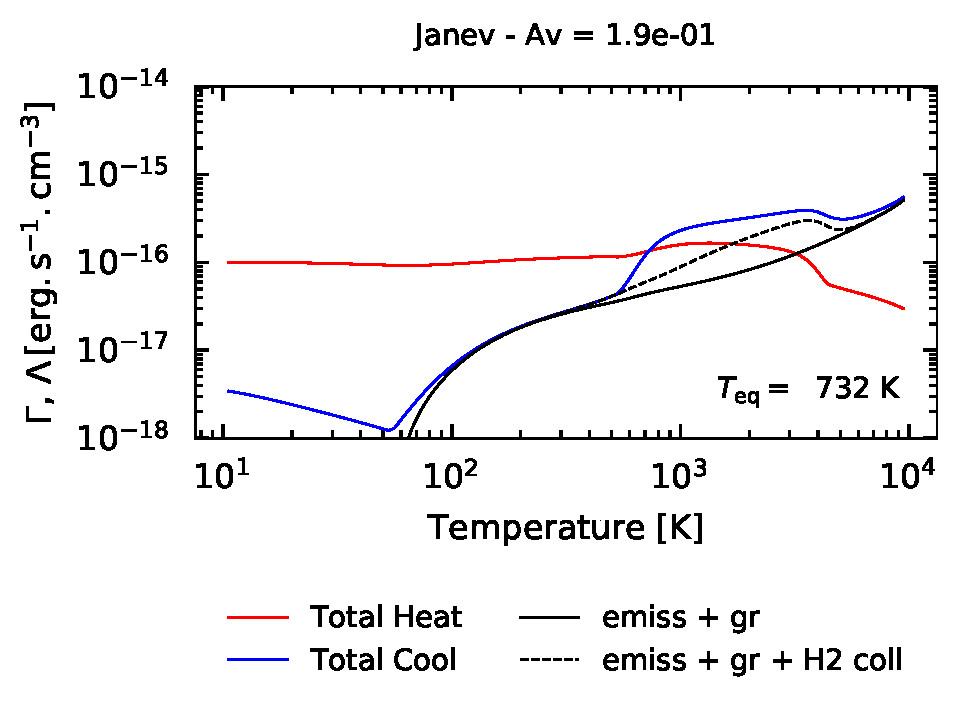
\includegraphics[trim = {0 0 0 1cm },clip,width=1\textwidth]{figure/H2/bosse_dcte_janevVSglover/janev/GC_c_1p9em01.pdf}
        \caption{Janev}
    \end{subfigure}
    \begin{subfigure}[t]{0.49\textwidth}
        \centering 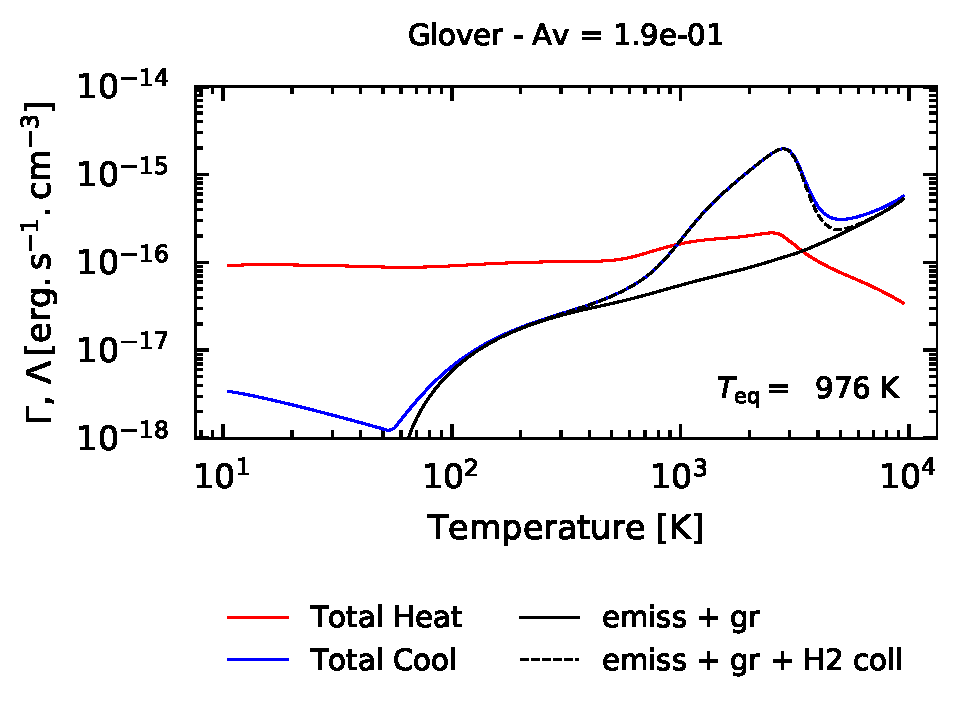
\includegraphics[trim = {0 0 0 1cm },clip,width=1\textwidth]{figure/H2/bosse_dcte_janevVSglover/glover/GC_c_1p9em01.pdf}
        \caption{Glover}
    \end{subfigure}
    \caption{(ANNEXE) Taux de chauffages et de refroidissements en fonction de la température à $A_\mathrm{v}$ de $0.2 \ \mathrm{mag}$ pour un modèle à densité constante ($n_\mathrm{H} = 10^{5.5}$ et $\chi = 10^4$).}
    \label{fig:H2:bosse:GC}
\end{figure}

\begin{figure}[!h]
    \centering
    \begin{subfigure}[t]{0.49\textwidth} % "0.49" donne ici la largeur de l'image
        \centering 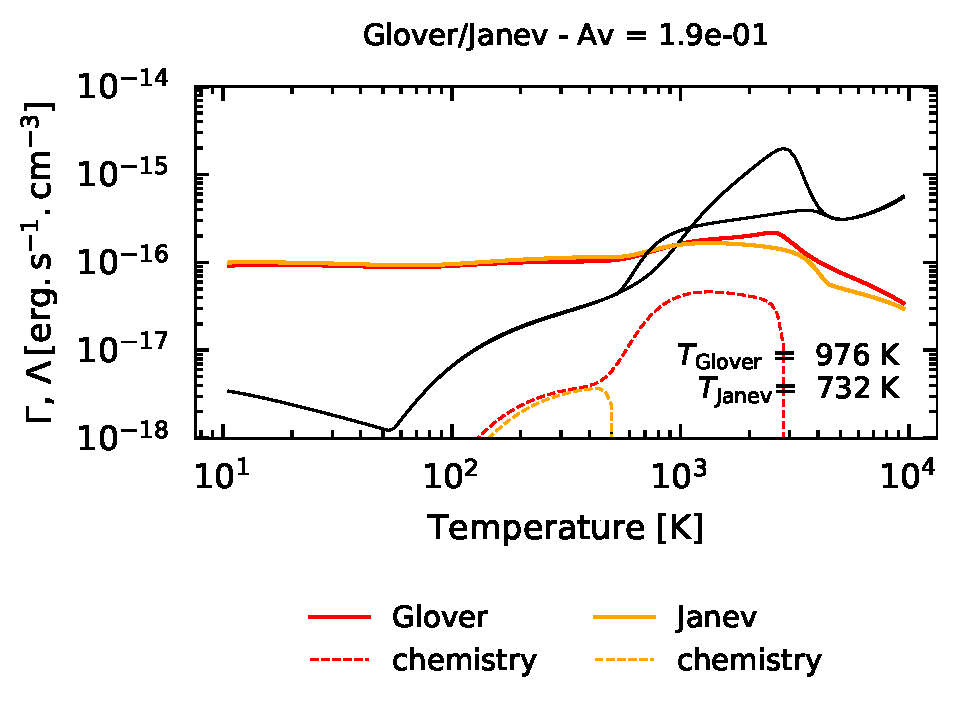
\includegraphics[trim = {0 0 0 1cm },clip,width=1\textwidth]{figure/H2/bosse_dcte_janevVSglover/GCcomp_h_1p9em01.pdf}
        \caption{Chauffage}
    \end{subfigure}
    \begin{subfigure}[t]{0.49\textwidth}
        \centering 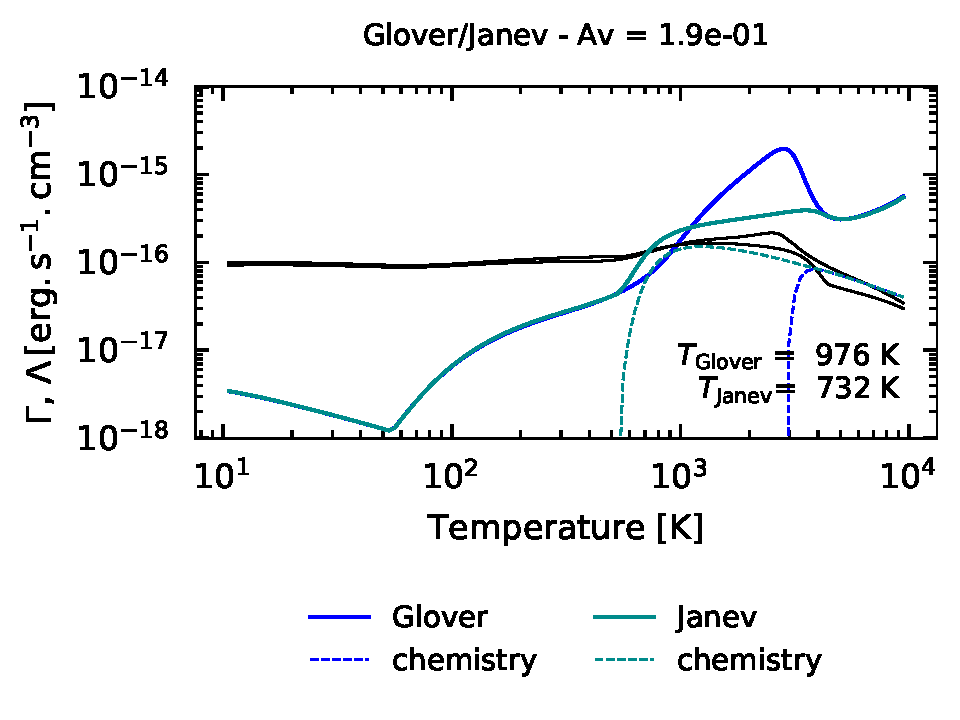
\includegraphics[trim = {0 0 0 1cm },clip,width=1\textwidth]{figure/H2/bosse_dcte_janevVSglover/GCcomp_c_1p9em01.pdf}
        \caption{Refroidissement}
    \end{subfigure}
    \caption{Efficacité du chauffage des réactions chimiques en fonction de la température pour un modèle à densité constante ($n_\mathrm{H} = 10^{5.5}$ et $\chi = 10^4$). Les courbes en rouge et jaune sur la figure (a) représente les processus de chauffage tandis que celles en noires les courbes de refroidissement total. Sur la figure (b), les courbes en bleu et bleu clair représentent le refroidissement alors que celles en noires le chauffage.}
    \label{fig:H2:bosse:chem}
\end{figure}

L'augmentation de température est provoquée par le changement d'allure de la courbe de refroidissement total ce qui déplace le point d'équilibre vers des températures plus chaudes. La conséquence immédiate de cette bosse de température s'observe sur les diagrammes d'intensité du $\mathrm{CO}$ (figure \ref{fig:H2:bosse:ICO}). Les raies $ 8 \leq \mathrm{J}\leq 15$ doublent leur intensités tandis que les raies $\mathrm{J}\geq 15$ augmente d'un facteur 10 ce qui est important. <phrase sur la transition C+/C/CO ?>. On constate enfin que cette augmentation locale de température impacte les raies d'émissions du $\mathrm{CO}$ des PDR denses. 

\begin{figure}[!h]
    \centering
    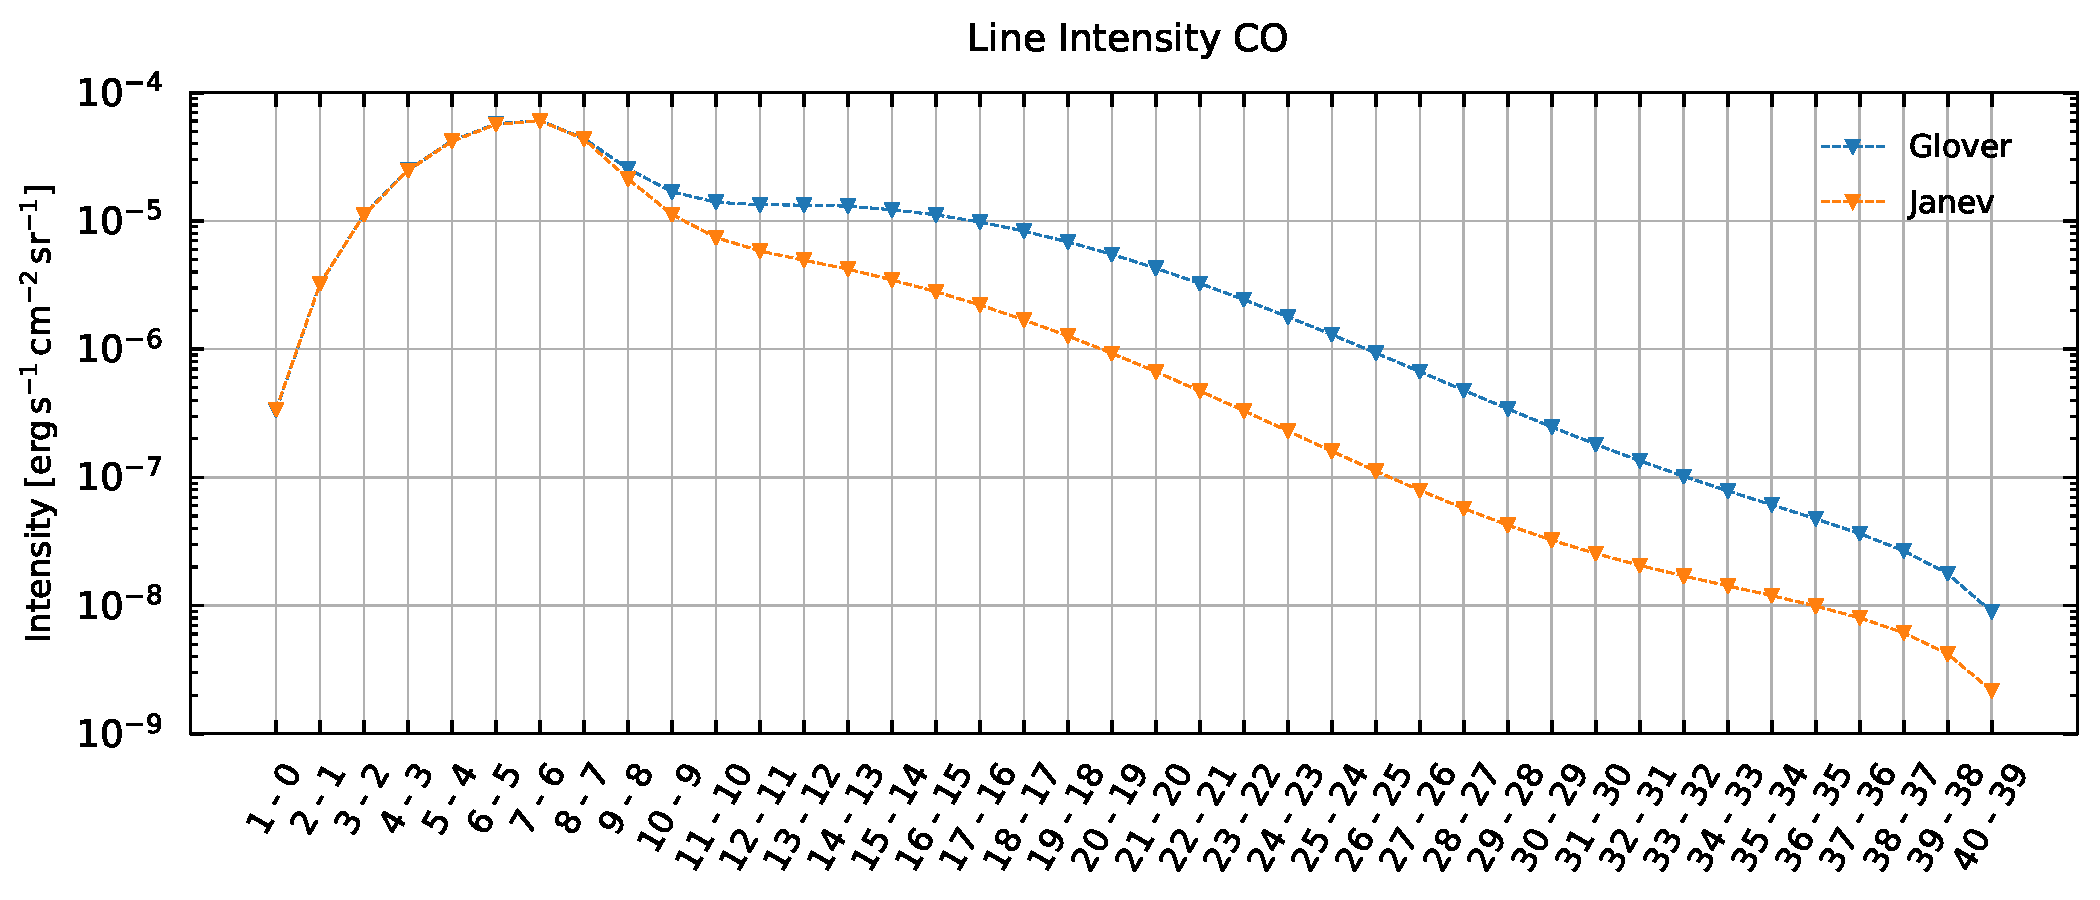
\includegraphics[trim = {0 0 0 1cm },clip,width=0.8\textwidth]{figure/H2/bosse_dcte_janevVSglover/I_comp_CO.pdf}
    \caption{Raies d'émissions du $\mathrm{CO}$ pour un modèle à densité constante ($n_\mathrm{H} = 10^{5.5}$ et $\chi = 10^4$) utilisant la prescription de Glover ou bien celle de Janev. Les transitions écrites sur l'axe des abscisses signifient les transitions des niveaux rotationnels de la molécule $\mathrm{CO}$.}
    \label{fig:H2:bosse:ICO}
\end{figure}



\begin{figure}[!h]
    \centering
    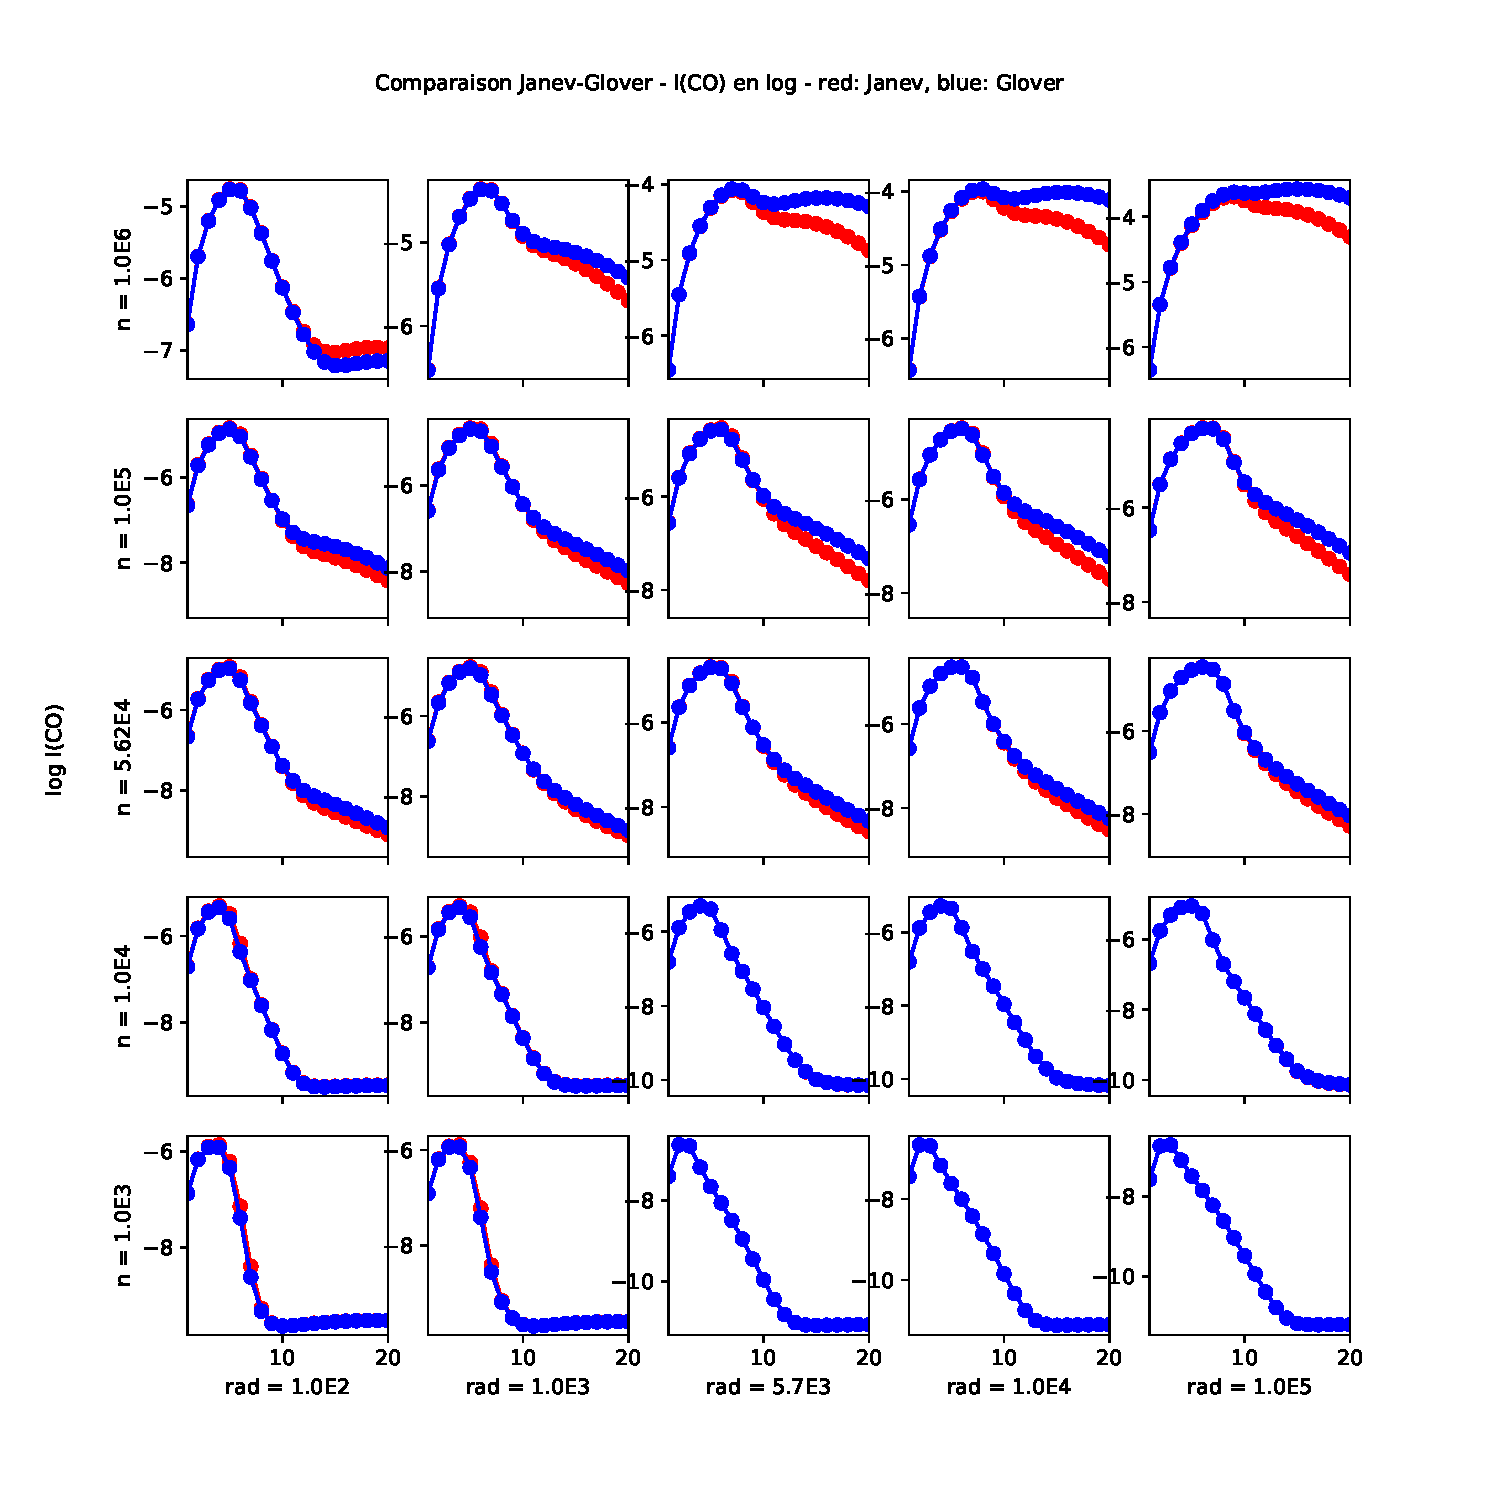
\includegraphics[trim = {0 0 0 3cm },clip,width=1\textwidth]{figure/H2/bosse_dcte_janevVSglover/PlotComp_Janev_Glover_IntCO.pdf}
    \caption{Raies d'émissions du $\mathrm{CO}$ pour une grille de à densité constante. Les lignes en rouge sont les modèles utilisant la prescription de Janev tandis que celles en bleues utilisent la prescription de Glover. Les $20$ premières transitions sont représentées.}
    \label{fig:H2:bosse:IgridCO}
\end{figure}

\subsubsubsection{Chauffage par exothermicité des réactions chimiques}



% \subsubsection{Raies du $\mathrm{CO}$ et $\mathrm{H}_2$ - Janev/Glover}
% à tracer en plus des profils de températures de modèles ...

% et on remarque plusieurs choses. Tout d'abord les raies d'émissions de $\mathrm{H}_2$ et $\mathrm{CO}$ sont augmentées (\autoref{figu:H2:..}). De plus le profil de température avec la nouvelle prescription (Glover) est modifié un tout petit peu au au bord (+100K) et un peu à l'entrée du nuage moléculaire (+400K) (\autoref{fig:H2:JanevGlover:emiss}). L'augmentation de la température à l'entrée du nuage moléculaire ($A_\mathrm{V} = 0.8$) provient du chauffage par exothermicité des réactions chimiques qui devient majeure (jusqu'à $50\%$ du chauffage total). Janev a tendance à surestimer les taux de dissociation qui sont toutes deux des réactions endothermiques et qui ont des efficacités de refroidissement les plus importantes. Les taux calculé par Glover réduisent leur refroidissement globale sur le nuage ce qui le chauffe. \newline 


% \begin{figure}[h!]
%     \centering
%     \begin{subfigure}[t]{0.49\textwidth} % "0.49" donne ici la largeur de l'image
%         \centering 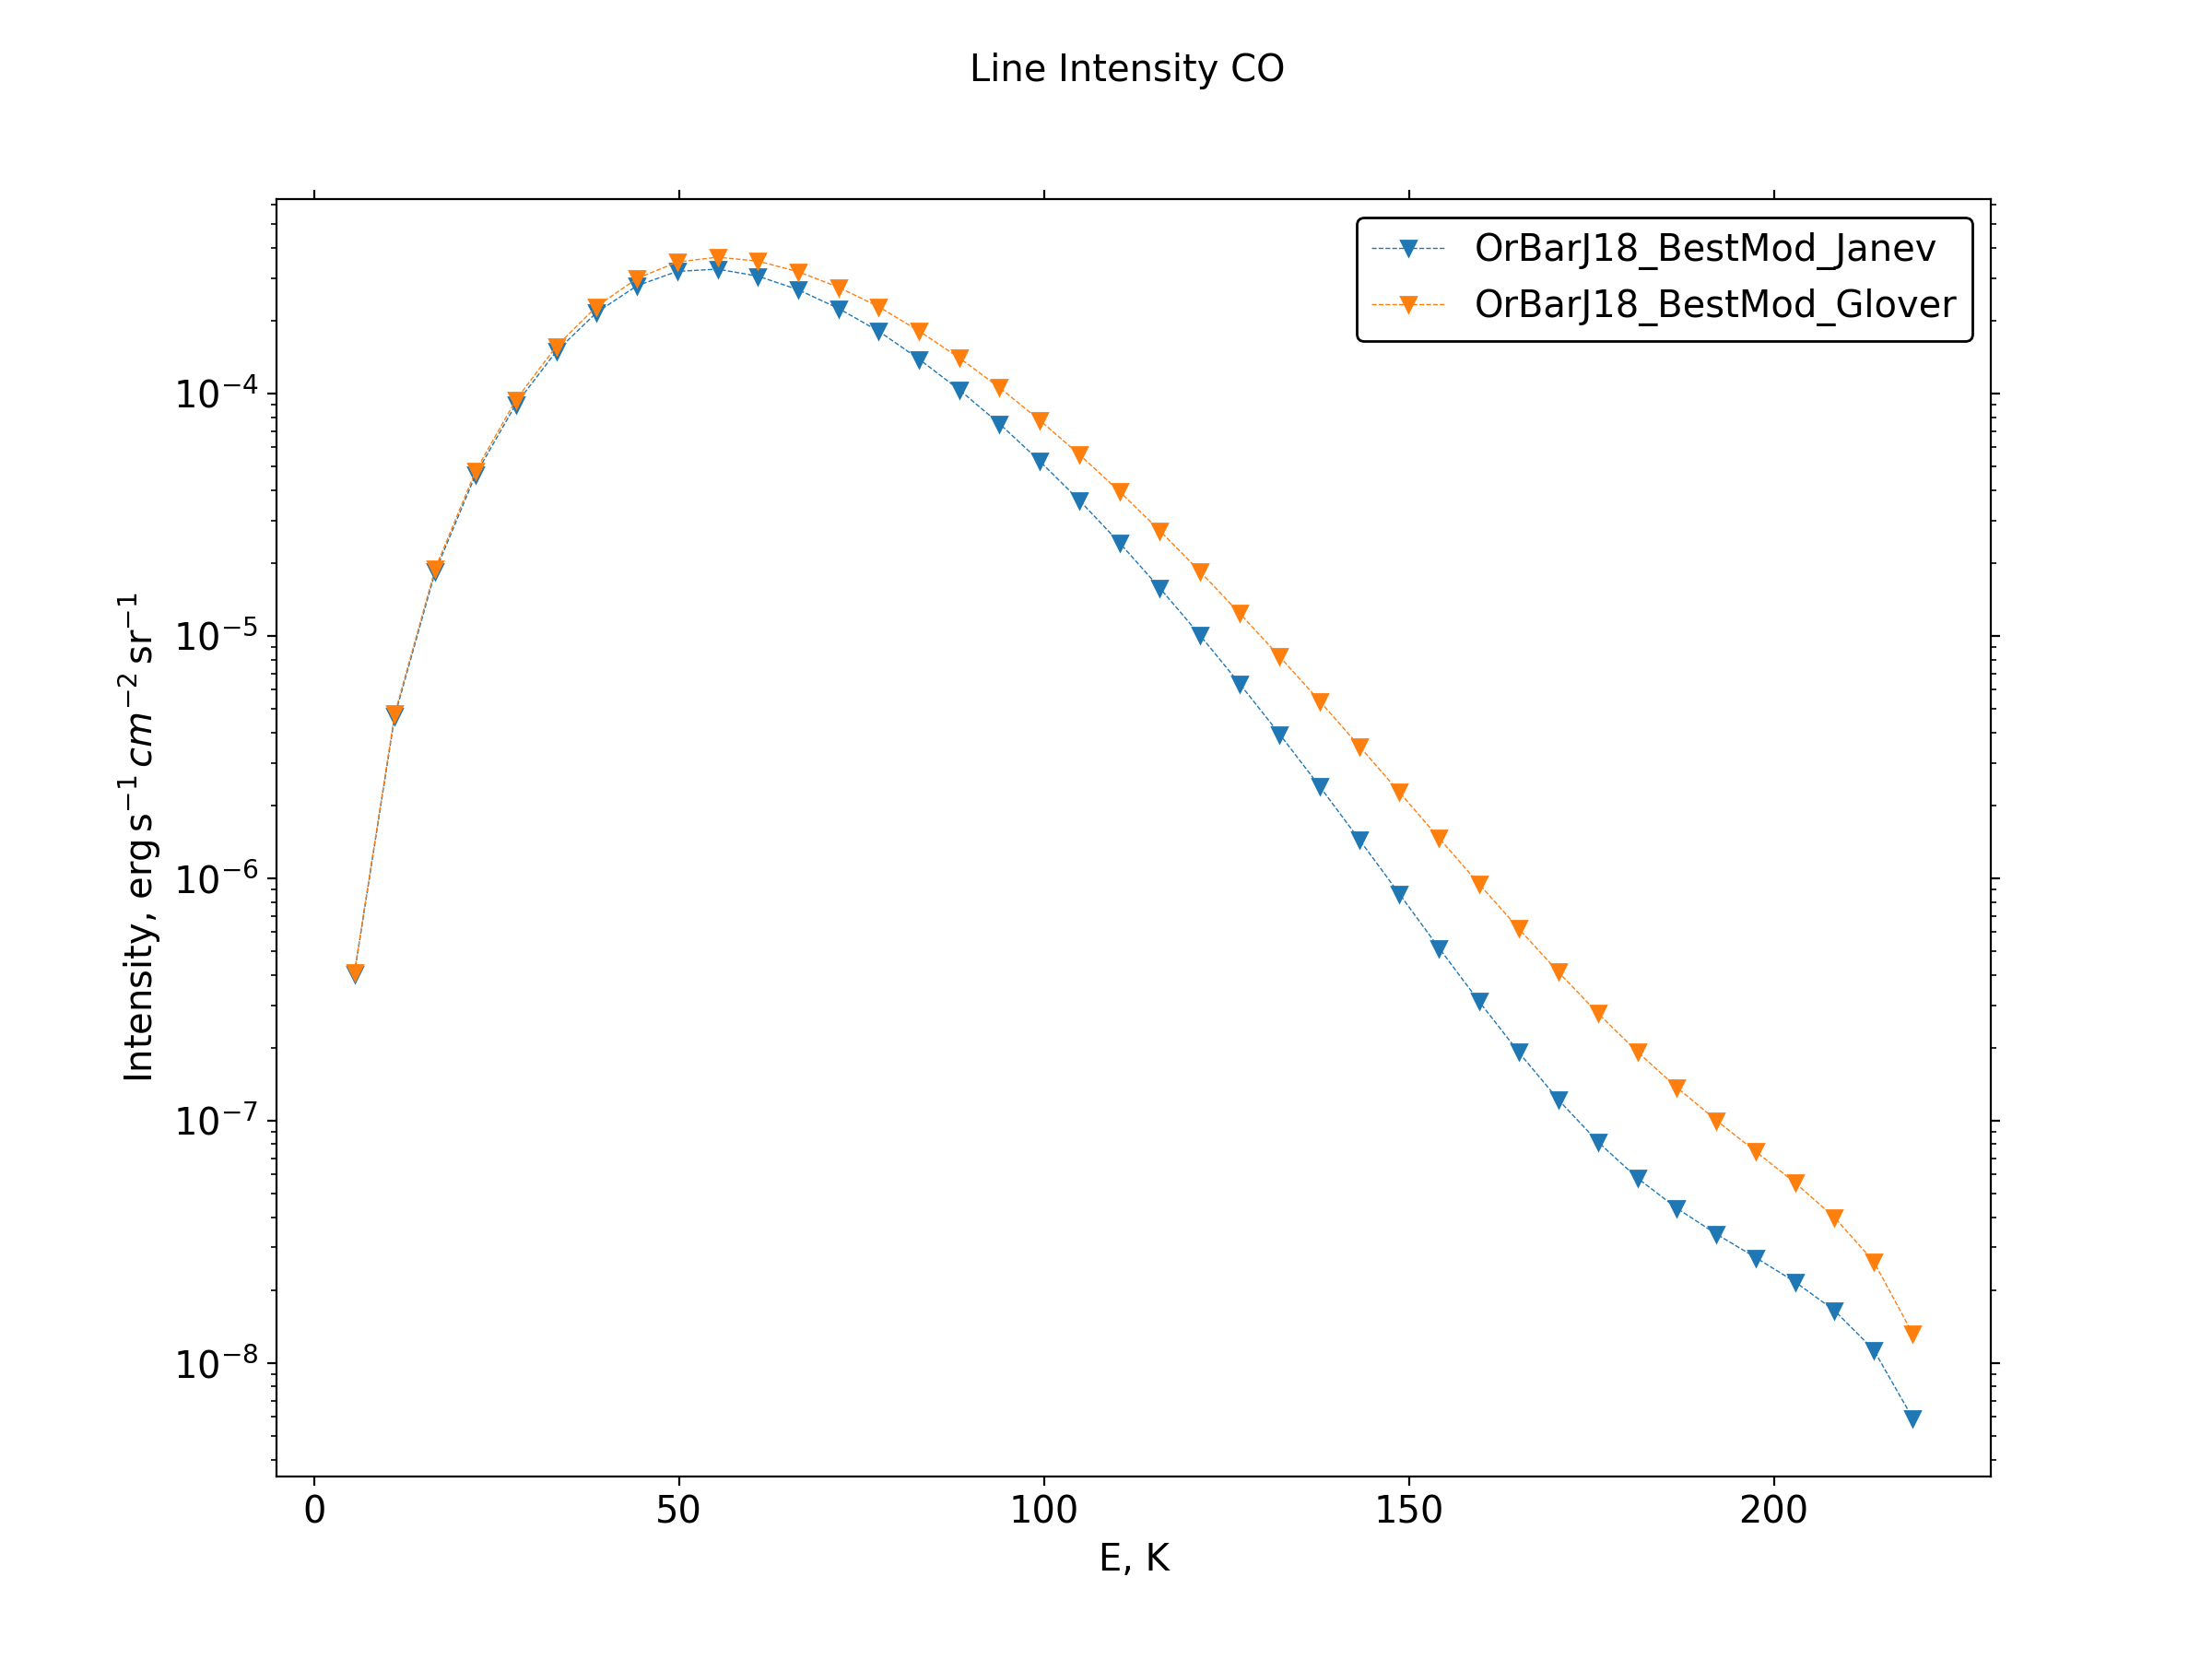
\includegraphics[trim = {0 0 0 1.5cm},clip,width=1\textwidth]{figure/H2/JanevGlover/I_comp_CO.png}
%         \caption{Spectre $\mathrm{H}_2$}
%     \end{subfigure}
%     ~ 
%     \begin{subfigure}[t]{0.49\textwidth}
%         \centering 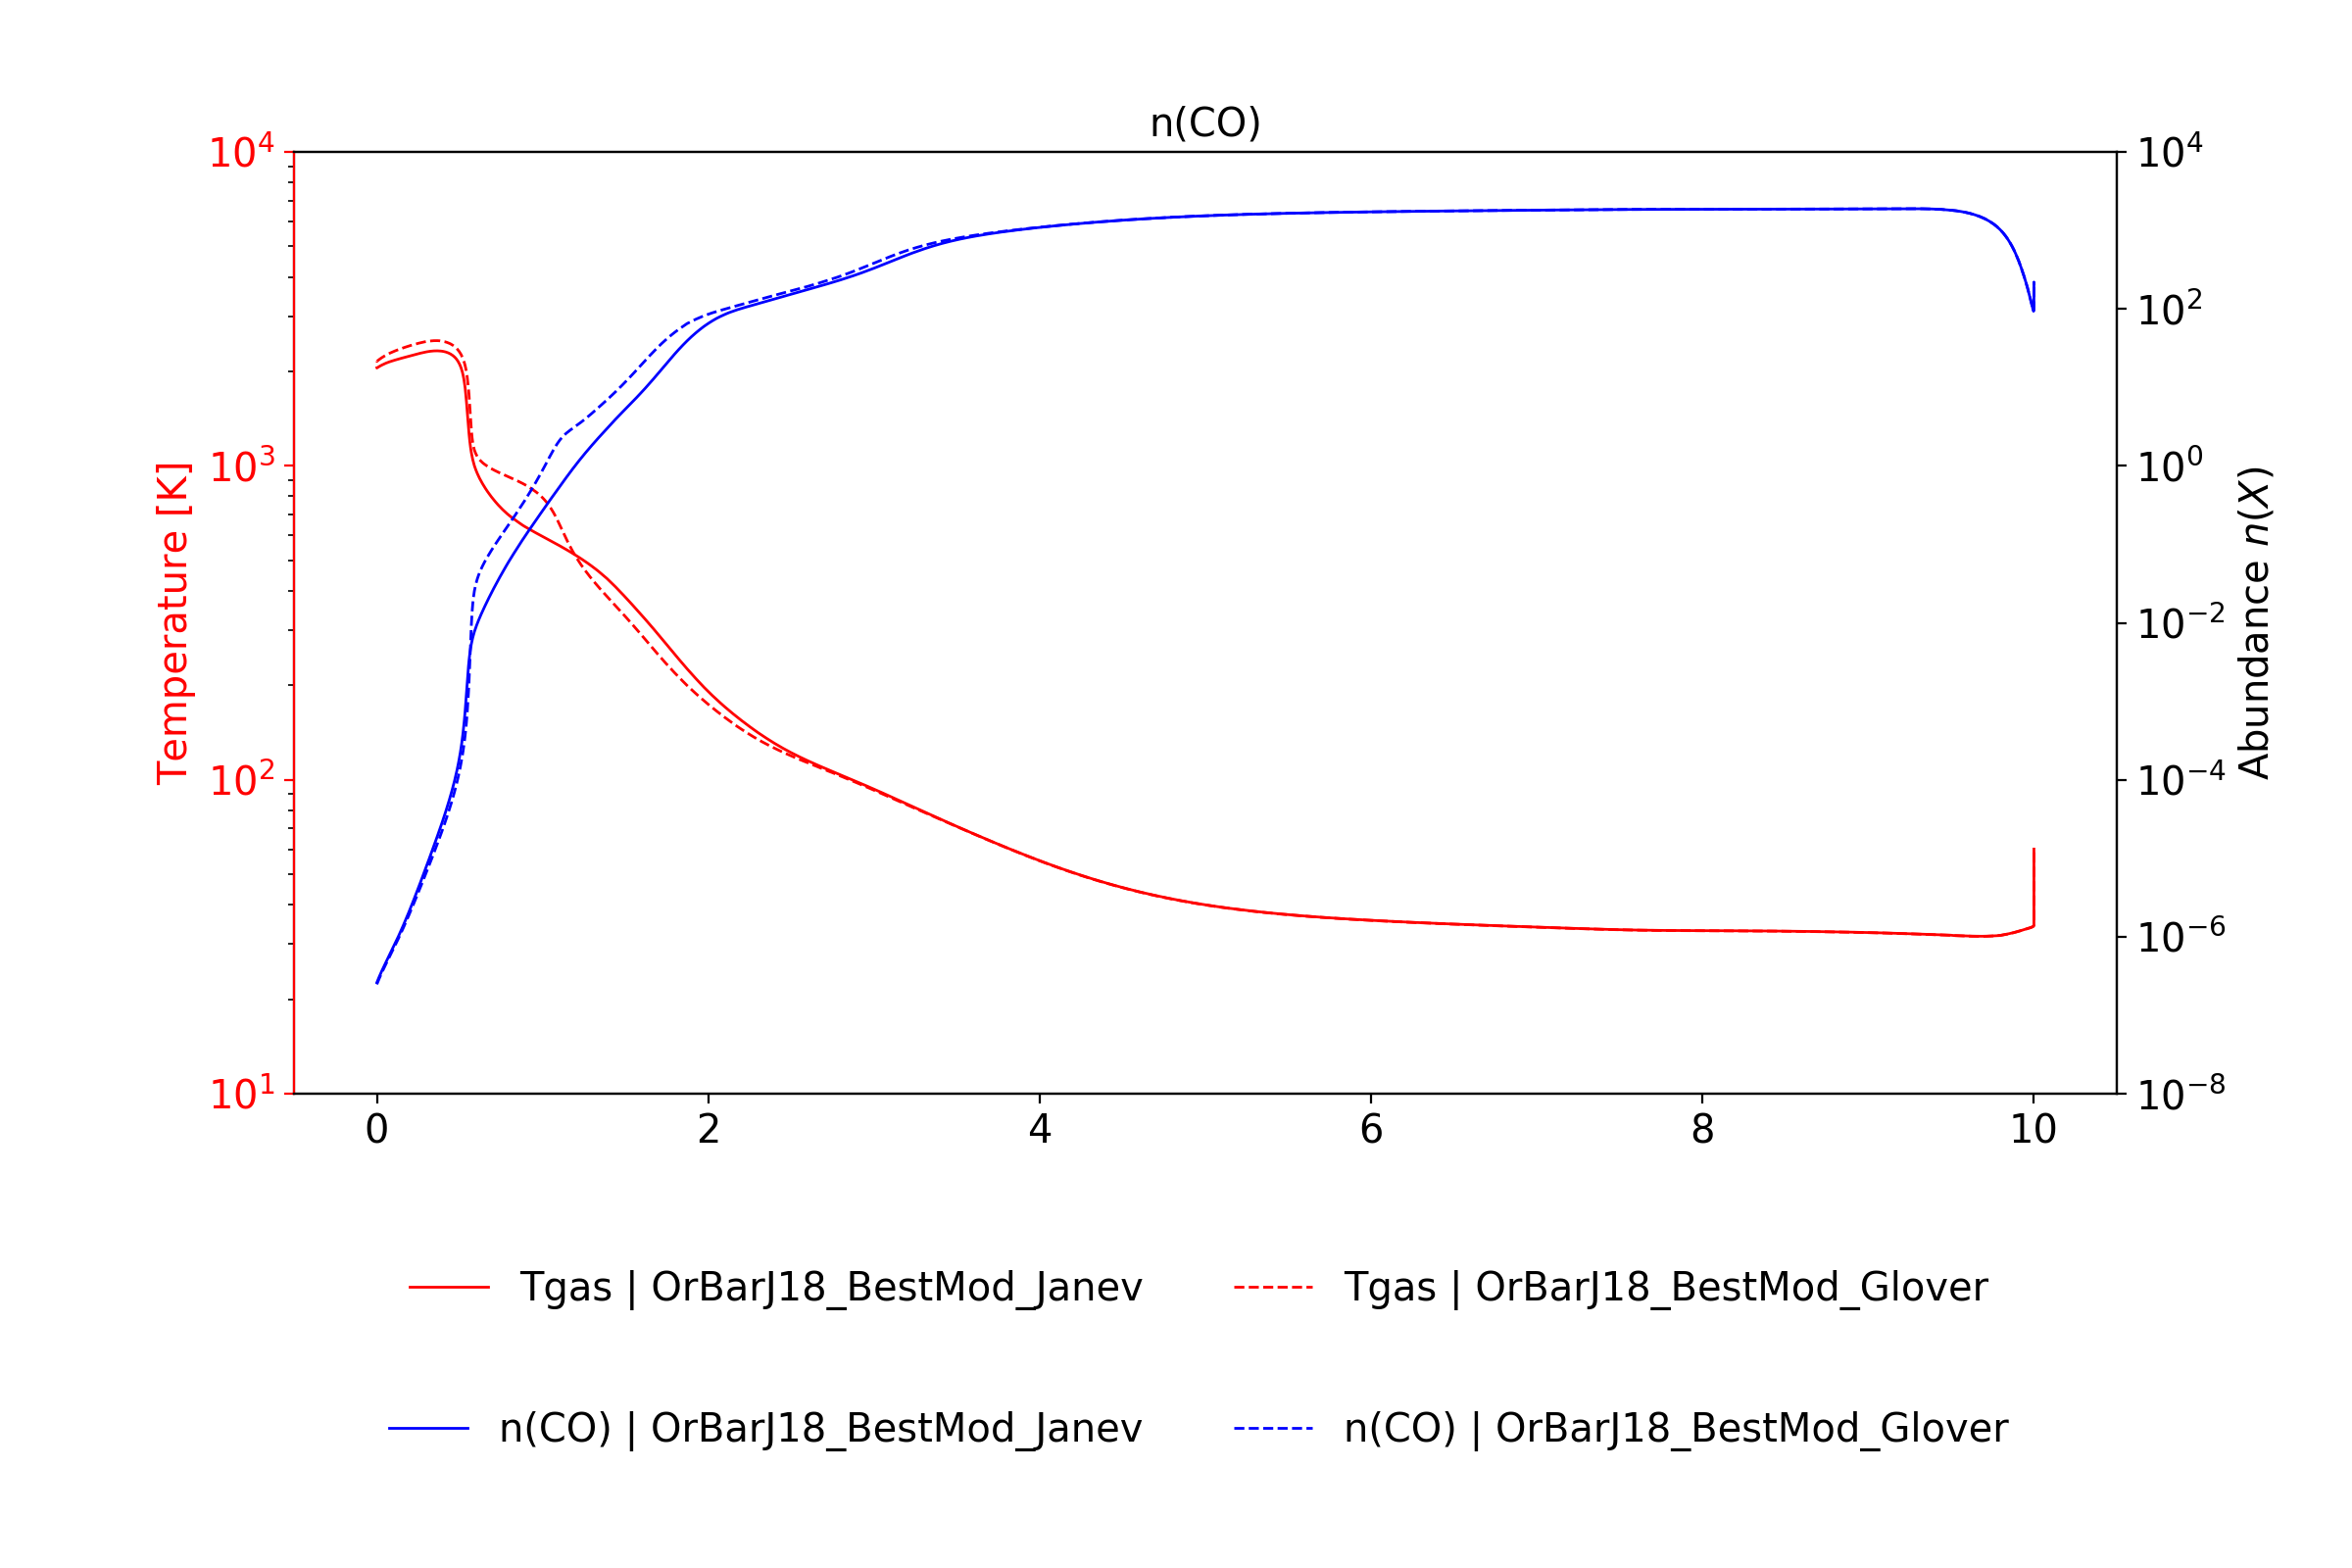
\includegraphics[trim = {0 0 0 1.5cm},clip,width=1\textwidth]{figure/H2/JanevGlover/nT_comp_CO.png}
%         \caption{Profil de densité et température de $\mathrm{H}_2$}
%     \end{subfigure}

%     \centering
%     \begin{subfigure}[t]{0.49\textwidth} % "0.49" donne ici la largeur de l'image
%         \centering 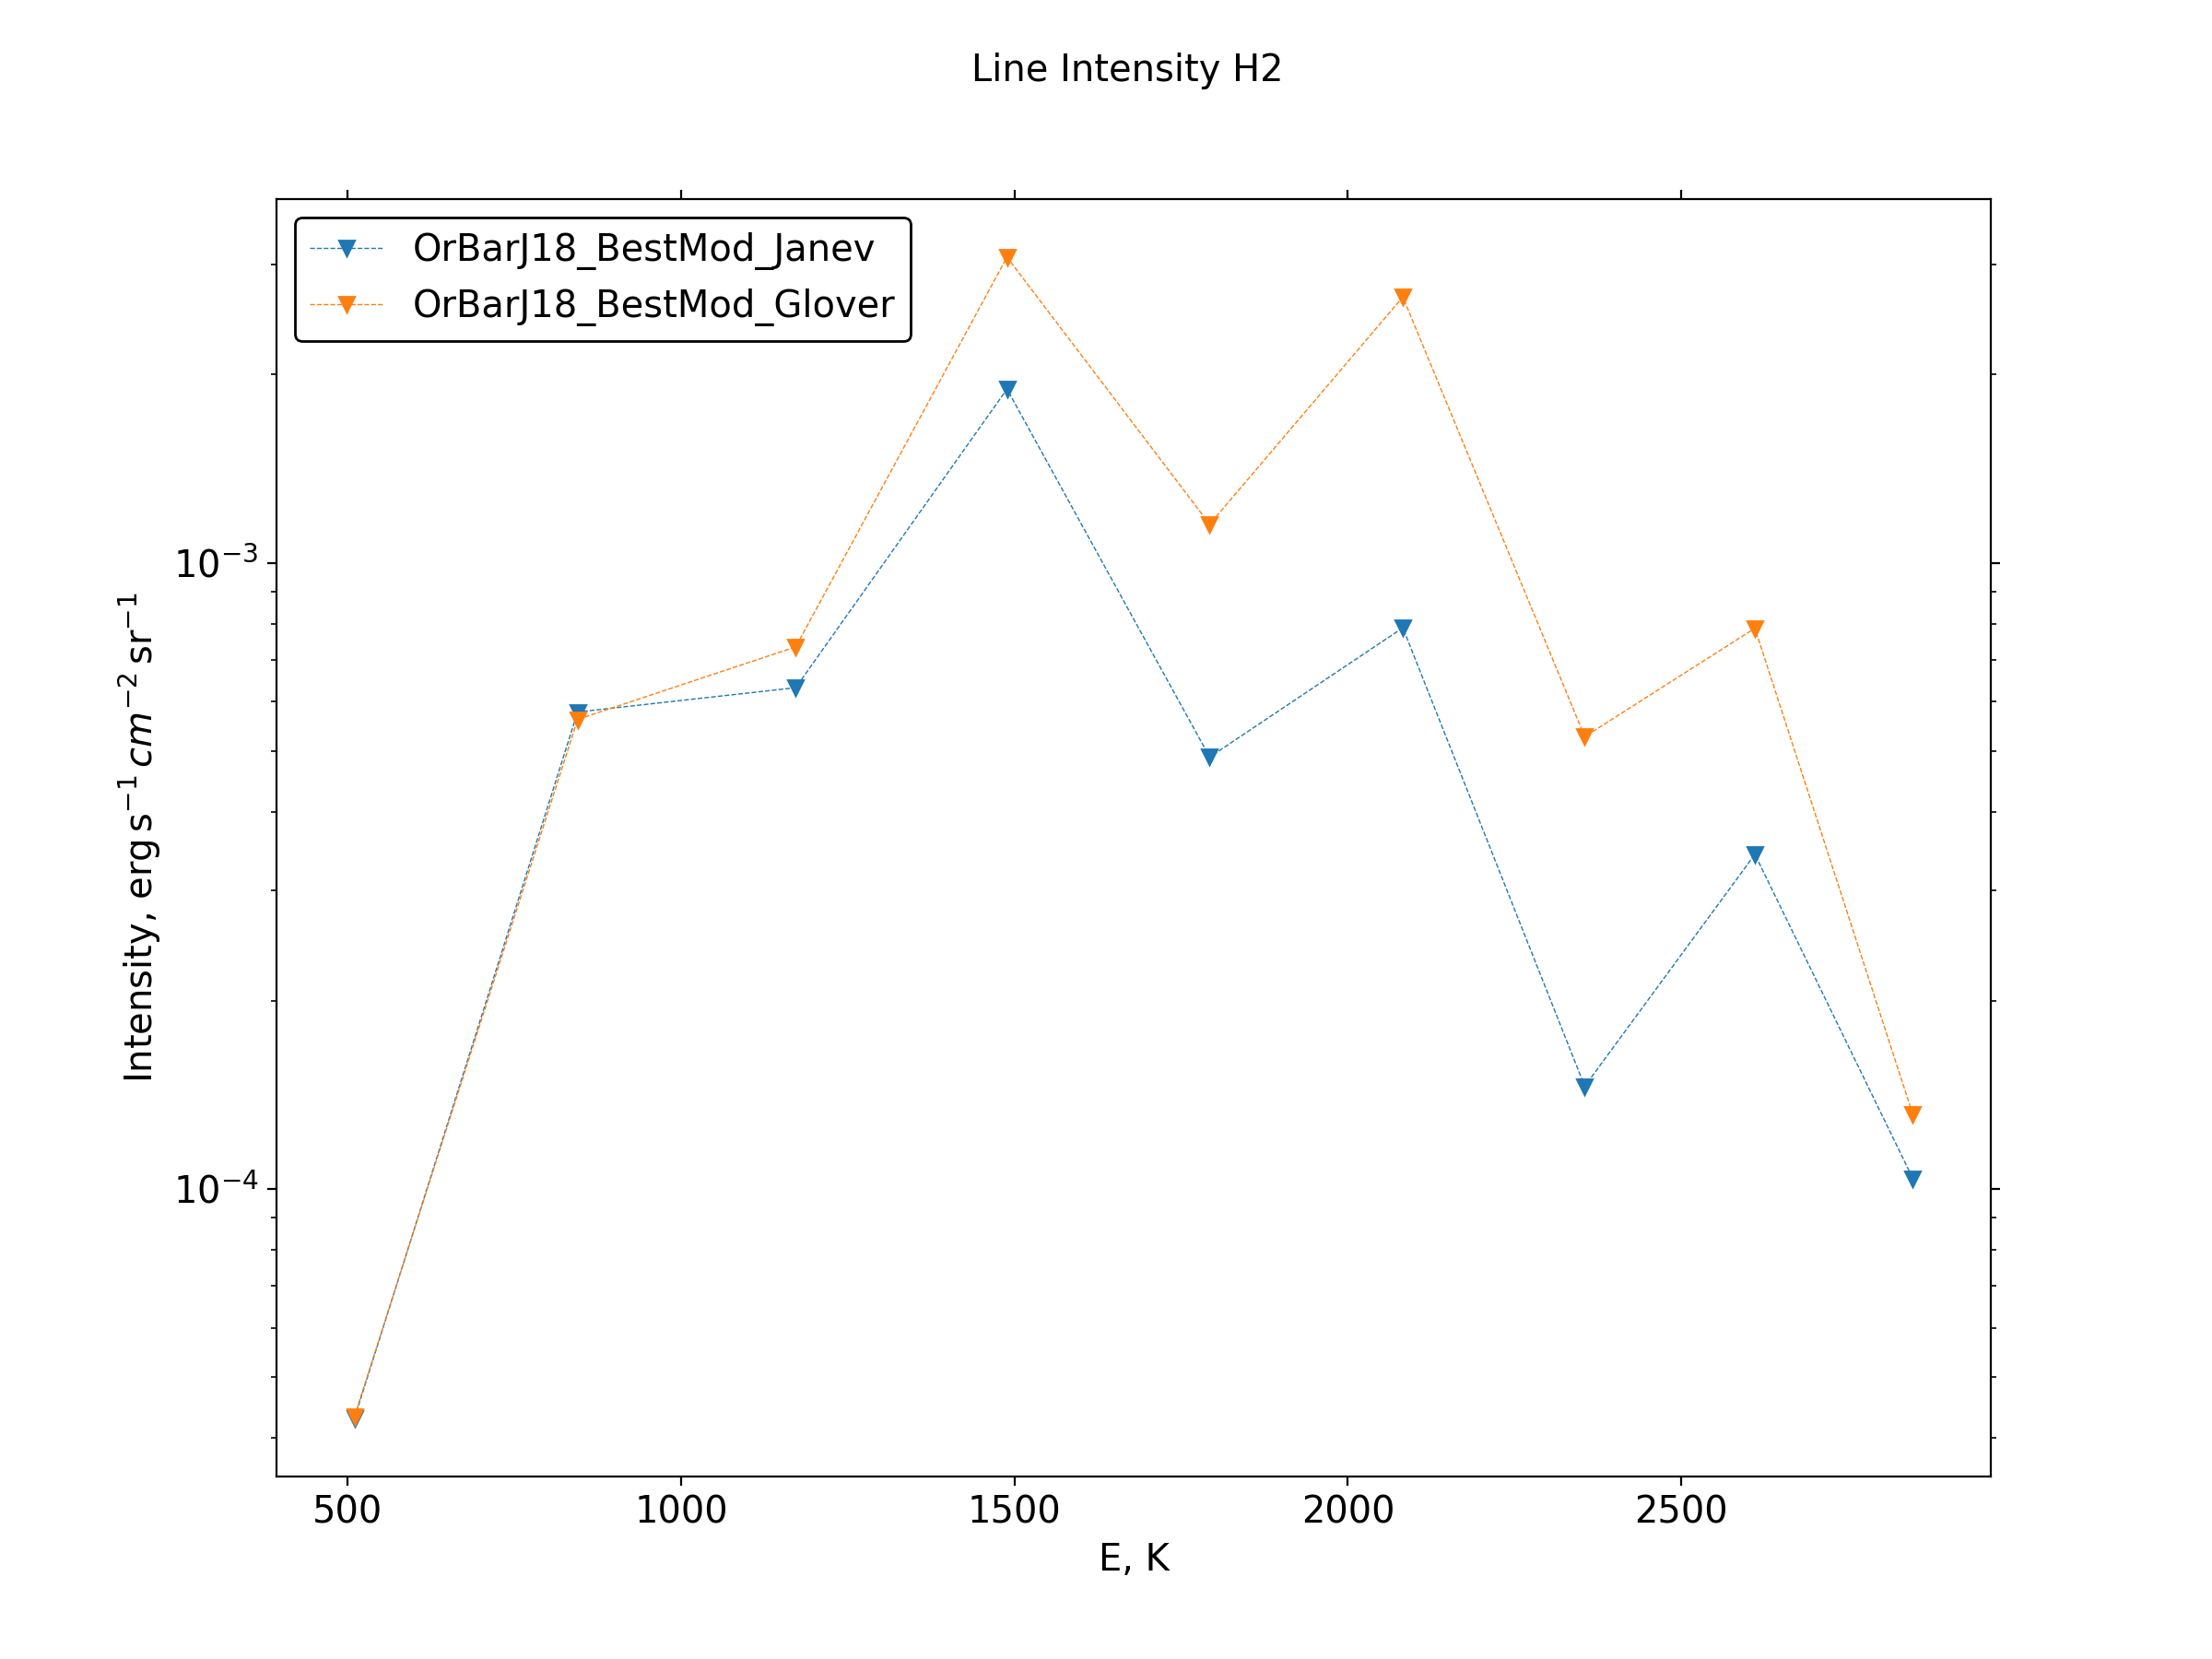
\includegraphics[trim = {0 0 0 1.5cm},clip,width=1\textwidth]{figure/H2/JanevGlover/I_comp_H2.png}
%         \caption{Spectre de $\mathrm{CO}$}
%     \end{subfigure}
%     ~ 
%     \begin{subfigure}[t]{0.49\textwidth}
%         \centering 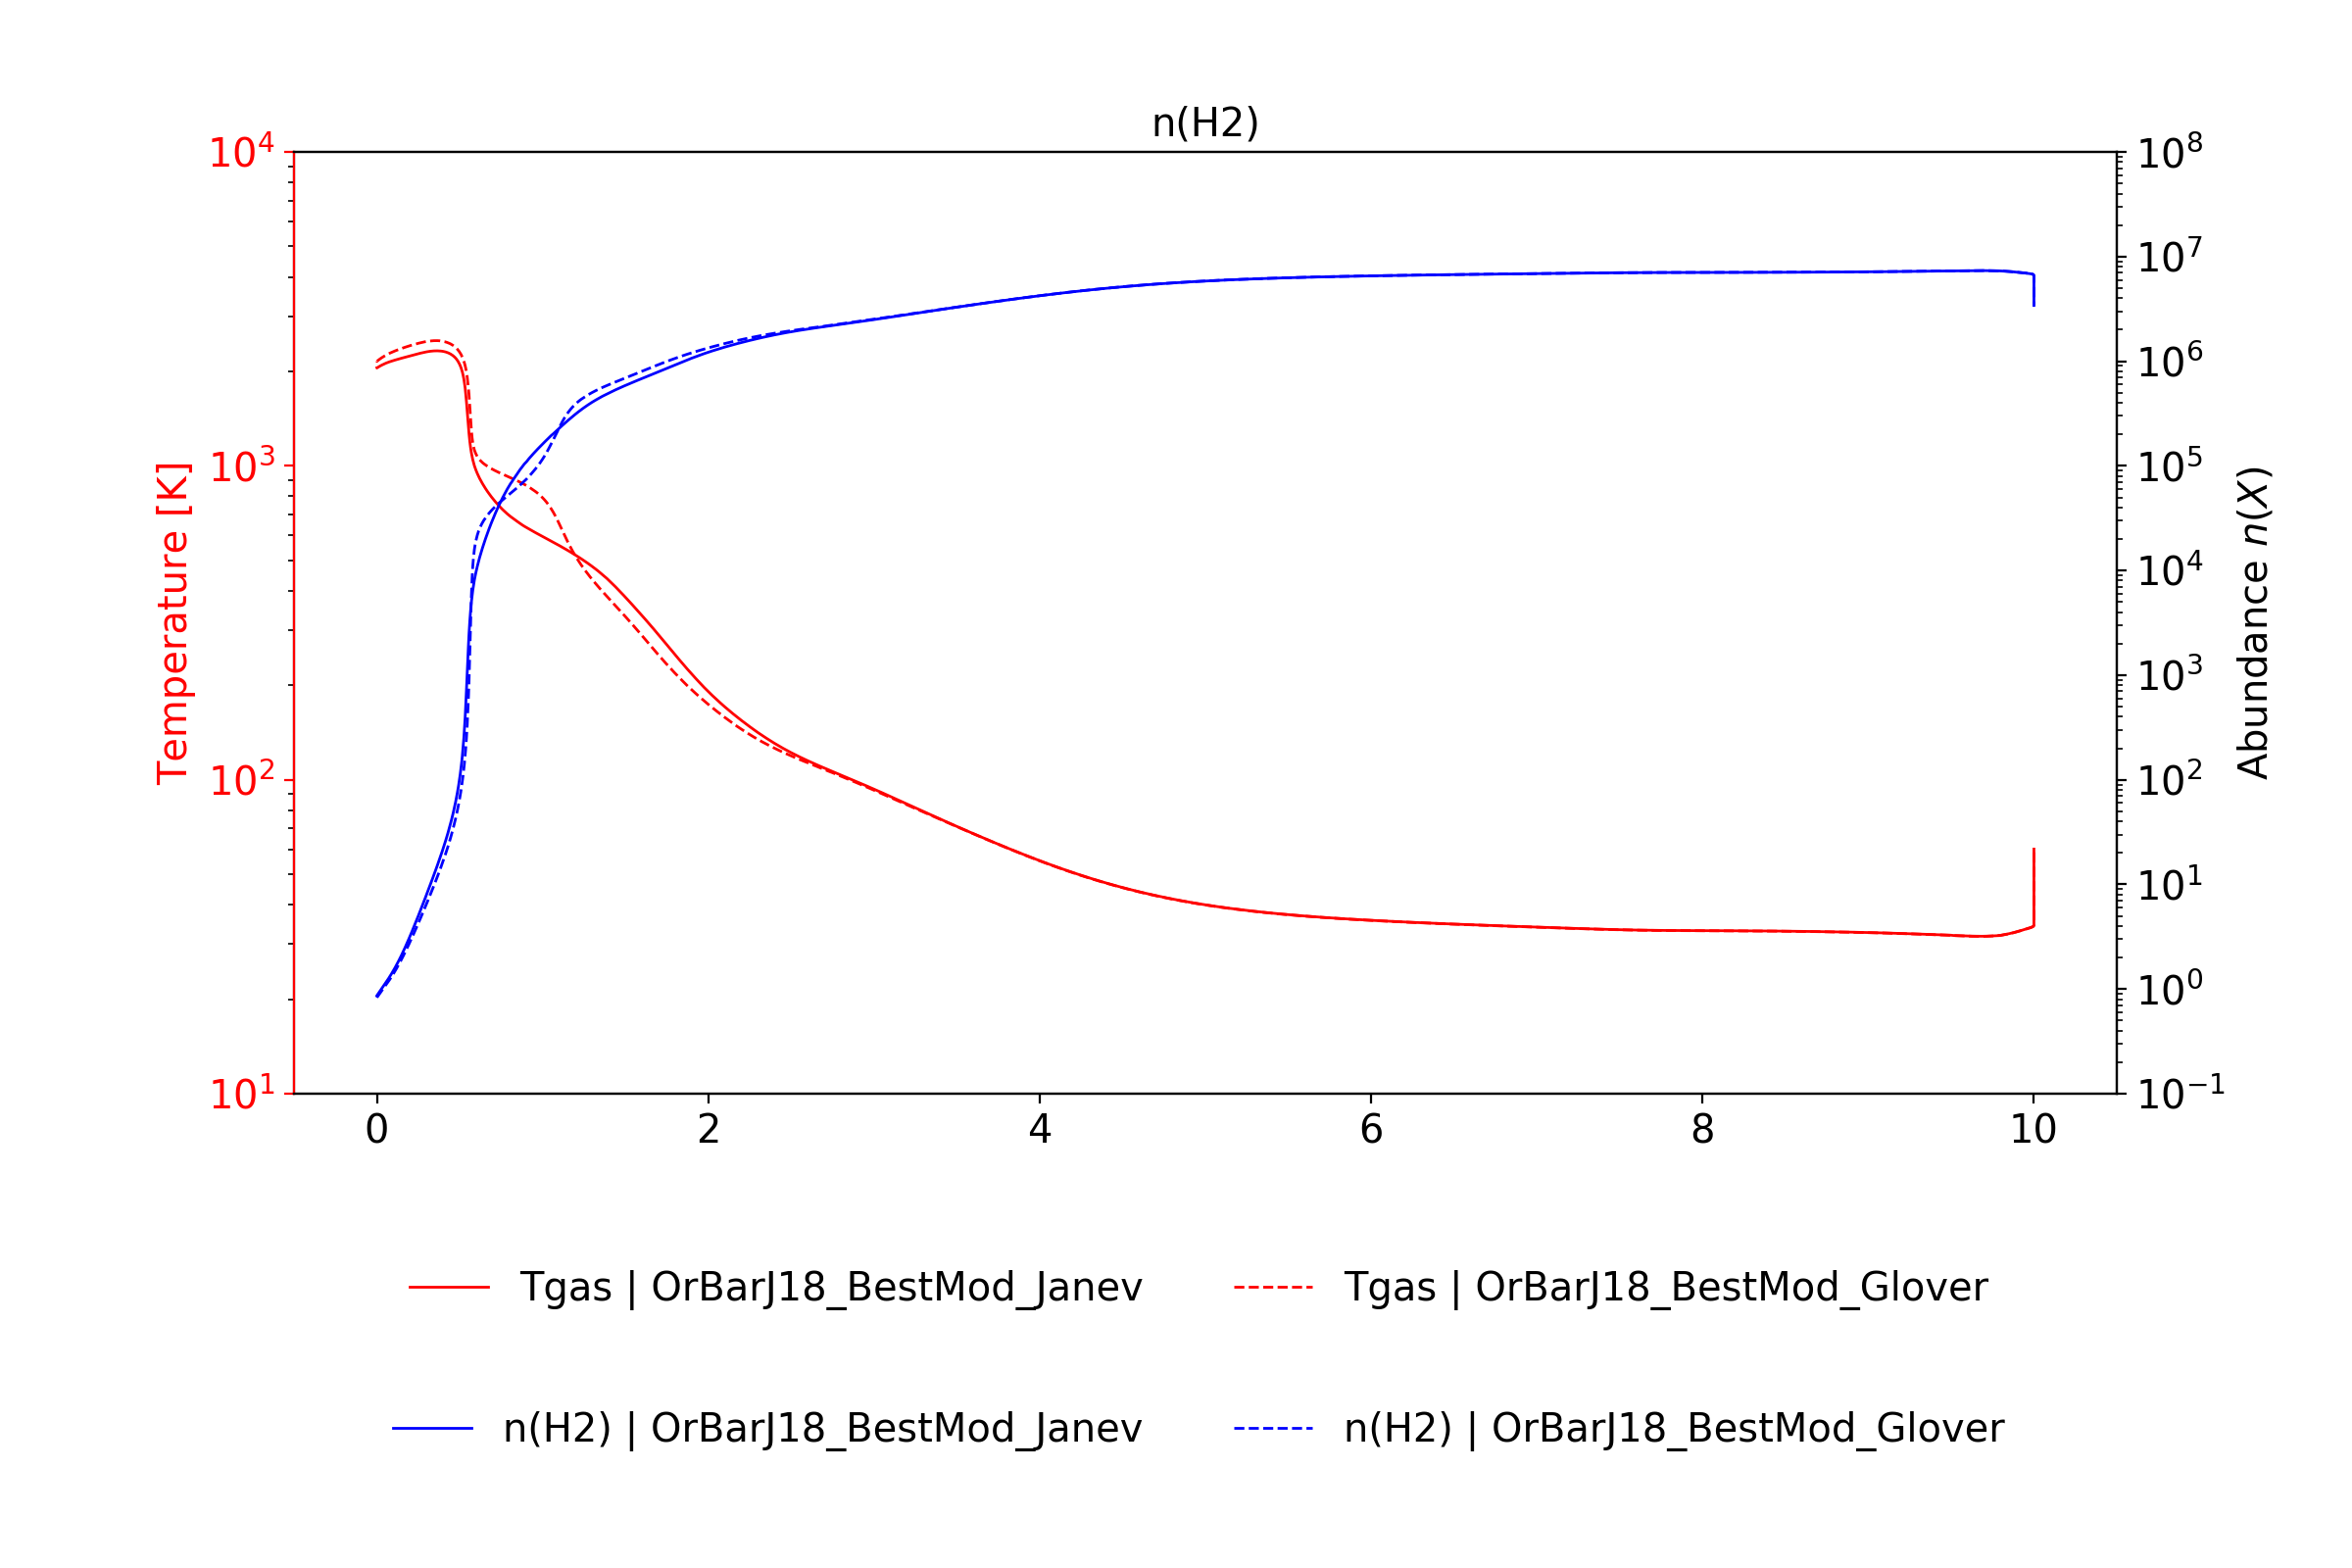
\includegraphics[trim = {0 0 0 1.5cm},clip,width=1\textwidth]{figure/H2/JanevGlover/nT_comp_H2.png}
%         \caption{Profil de densité et température de $\mathrm{CO}$}
%     \end{subfigure}
%     \caption{Impact des prescriptions de Janev et Glover sur les raies d'émissions des traceurs $\mathrm{H}_2$ et $\mathrm{CO}$}
%     \label{fig:H2:JanevGlover:emiss}
% \end{figure}


% Néanmoins on connaît mal la proportion effective qui chauffe le gaz par exothermicité. Il faut reprendre l'étude sur l'exothermicité des réactions chimiques en jouant sur la prescription. \newline 

% On cherche à visualiser l'impact des nouveaux calculs des niveaux de $\mathrm{H}_2$ sur les raies. On l'a calculé dans le cas de Janev et Glover mais l'on montre seulement la prescription de Glover qui est la plus importante (\autoref{fig:H2:GloverBossion:emiss})

% On se rend compte que l'impact est minime alors que le travail pour calculer ces niveaux est lourd. Au moins on sait que connaître précisément les niveaux de $\mathrm{H}_2$ n'est pas décisif dans l'interprétation des spectres d'émissions. 

% \begin{figure}[h!]
%     \centering
%     \begin{subfigure}[t]{0.49\textwidth} % "0.49" donne ici la largeur de l'image
%         \centering 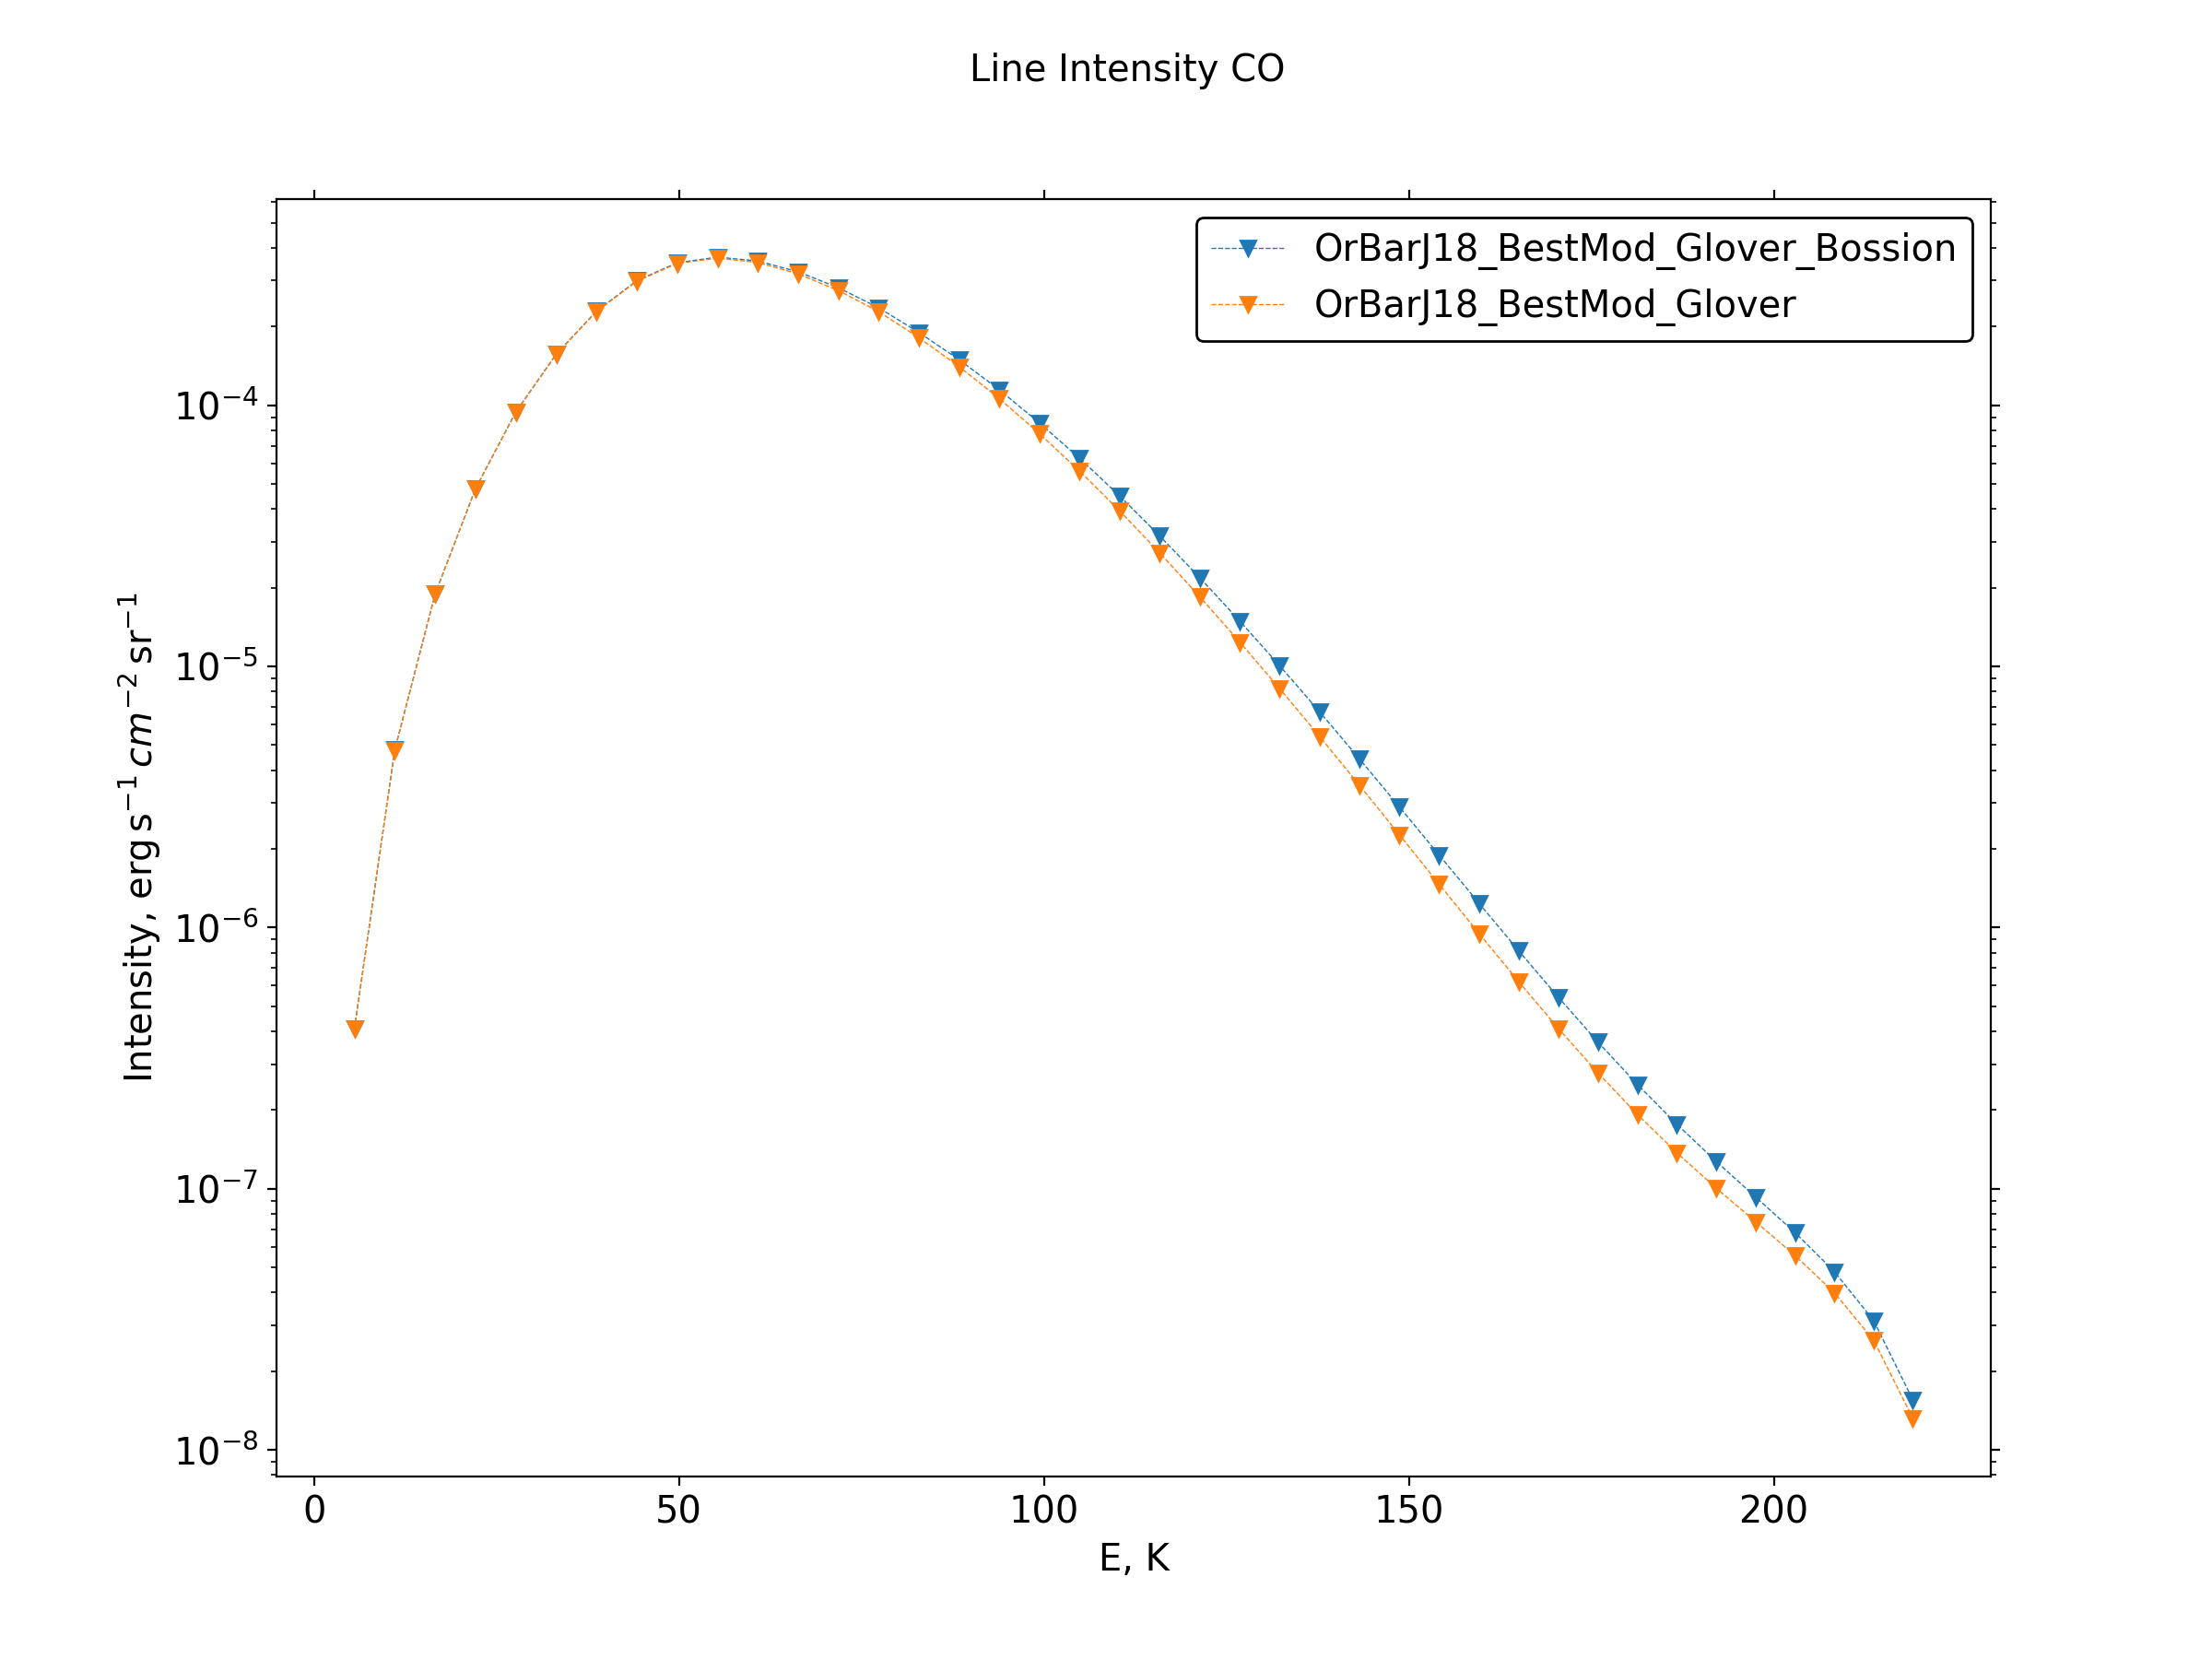
\includegraphics[trim = {0 0 0 1.5cm},clip,width=1\textwidth]{figure/H2/GloverBossion/I_comp_CO.png}
%         \caption{Spectre $\mathrm{H}_2$}
%     \end{subfigure}
%     ~ 
%     \begin{subfigure}[t]{0.49\textwidth}
%         \centering 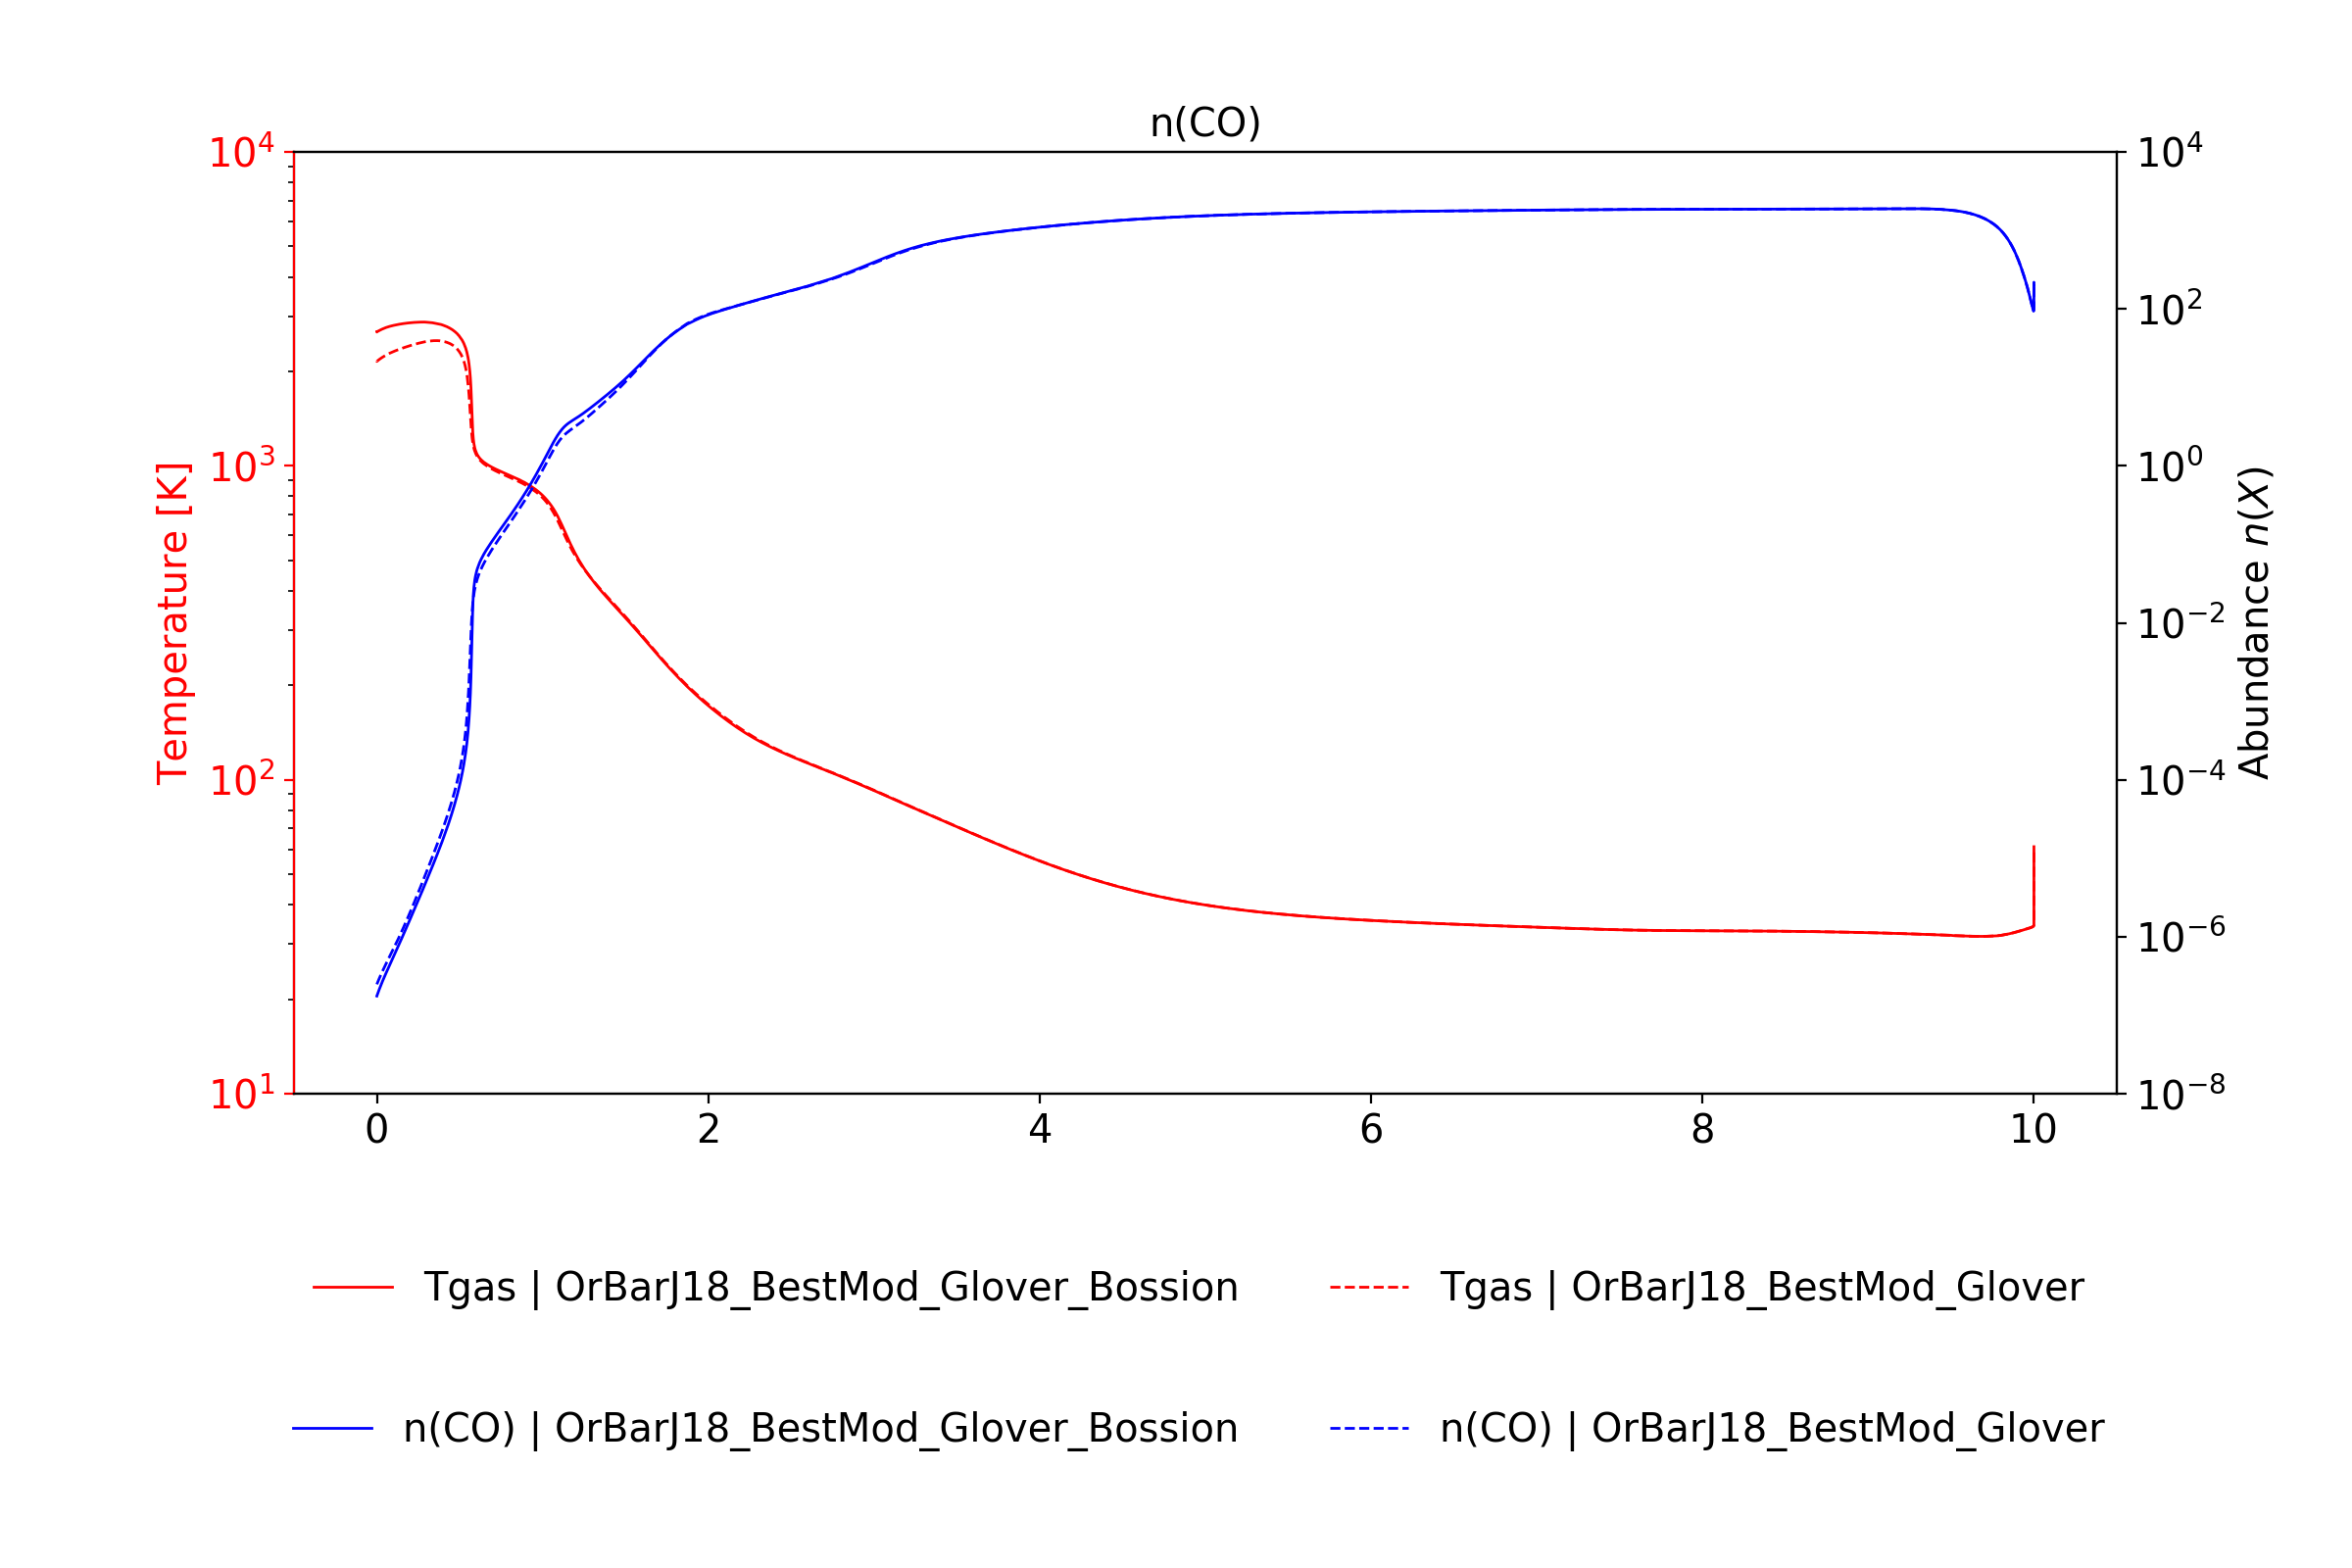
\includegraphics[trim = {0 0 0 1.5cm},clip,width=1\textwidth]{figure/H2/GloverBossion/nT_comp_CO.png}
%         \caption{Profil de densité et température de $\mathrm{H}_2$}
%     \end{subfigure}

%     \centering
%     \begin{subfigure}[t]{0.49\textwidth} % "0.49" donne ici la largeur de l'image
%         \centering 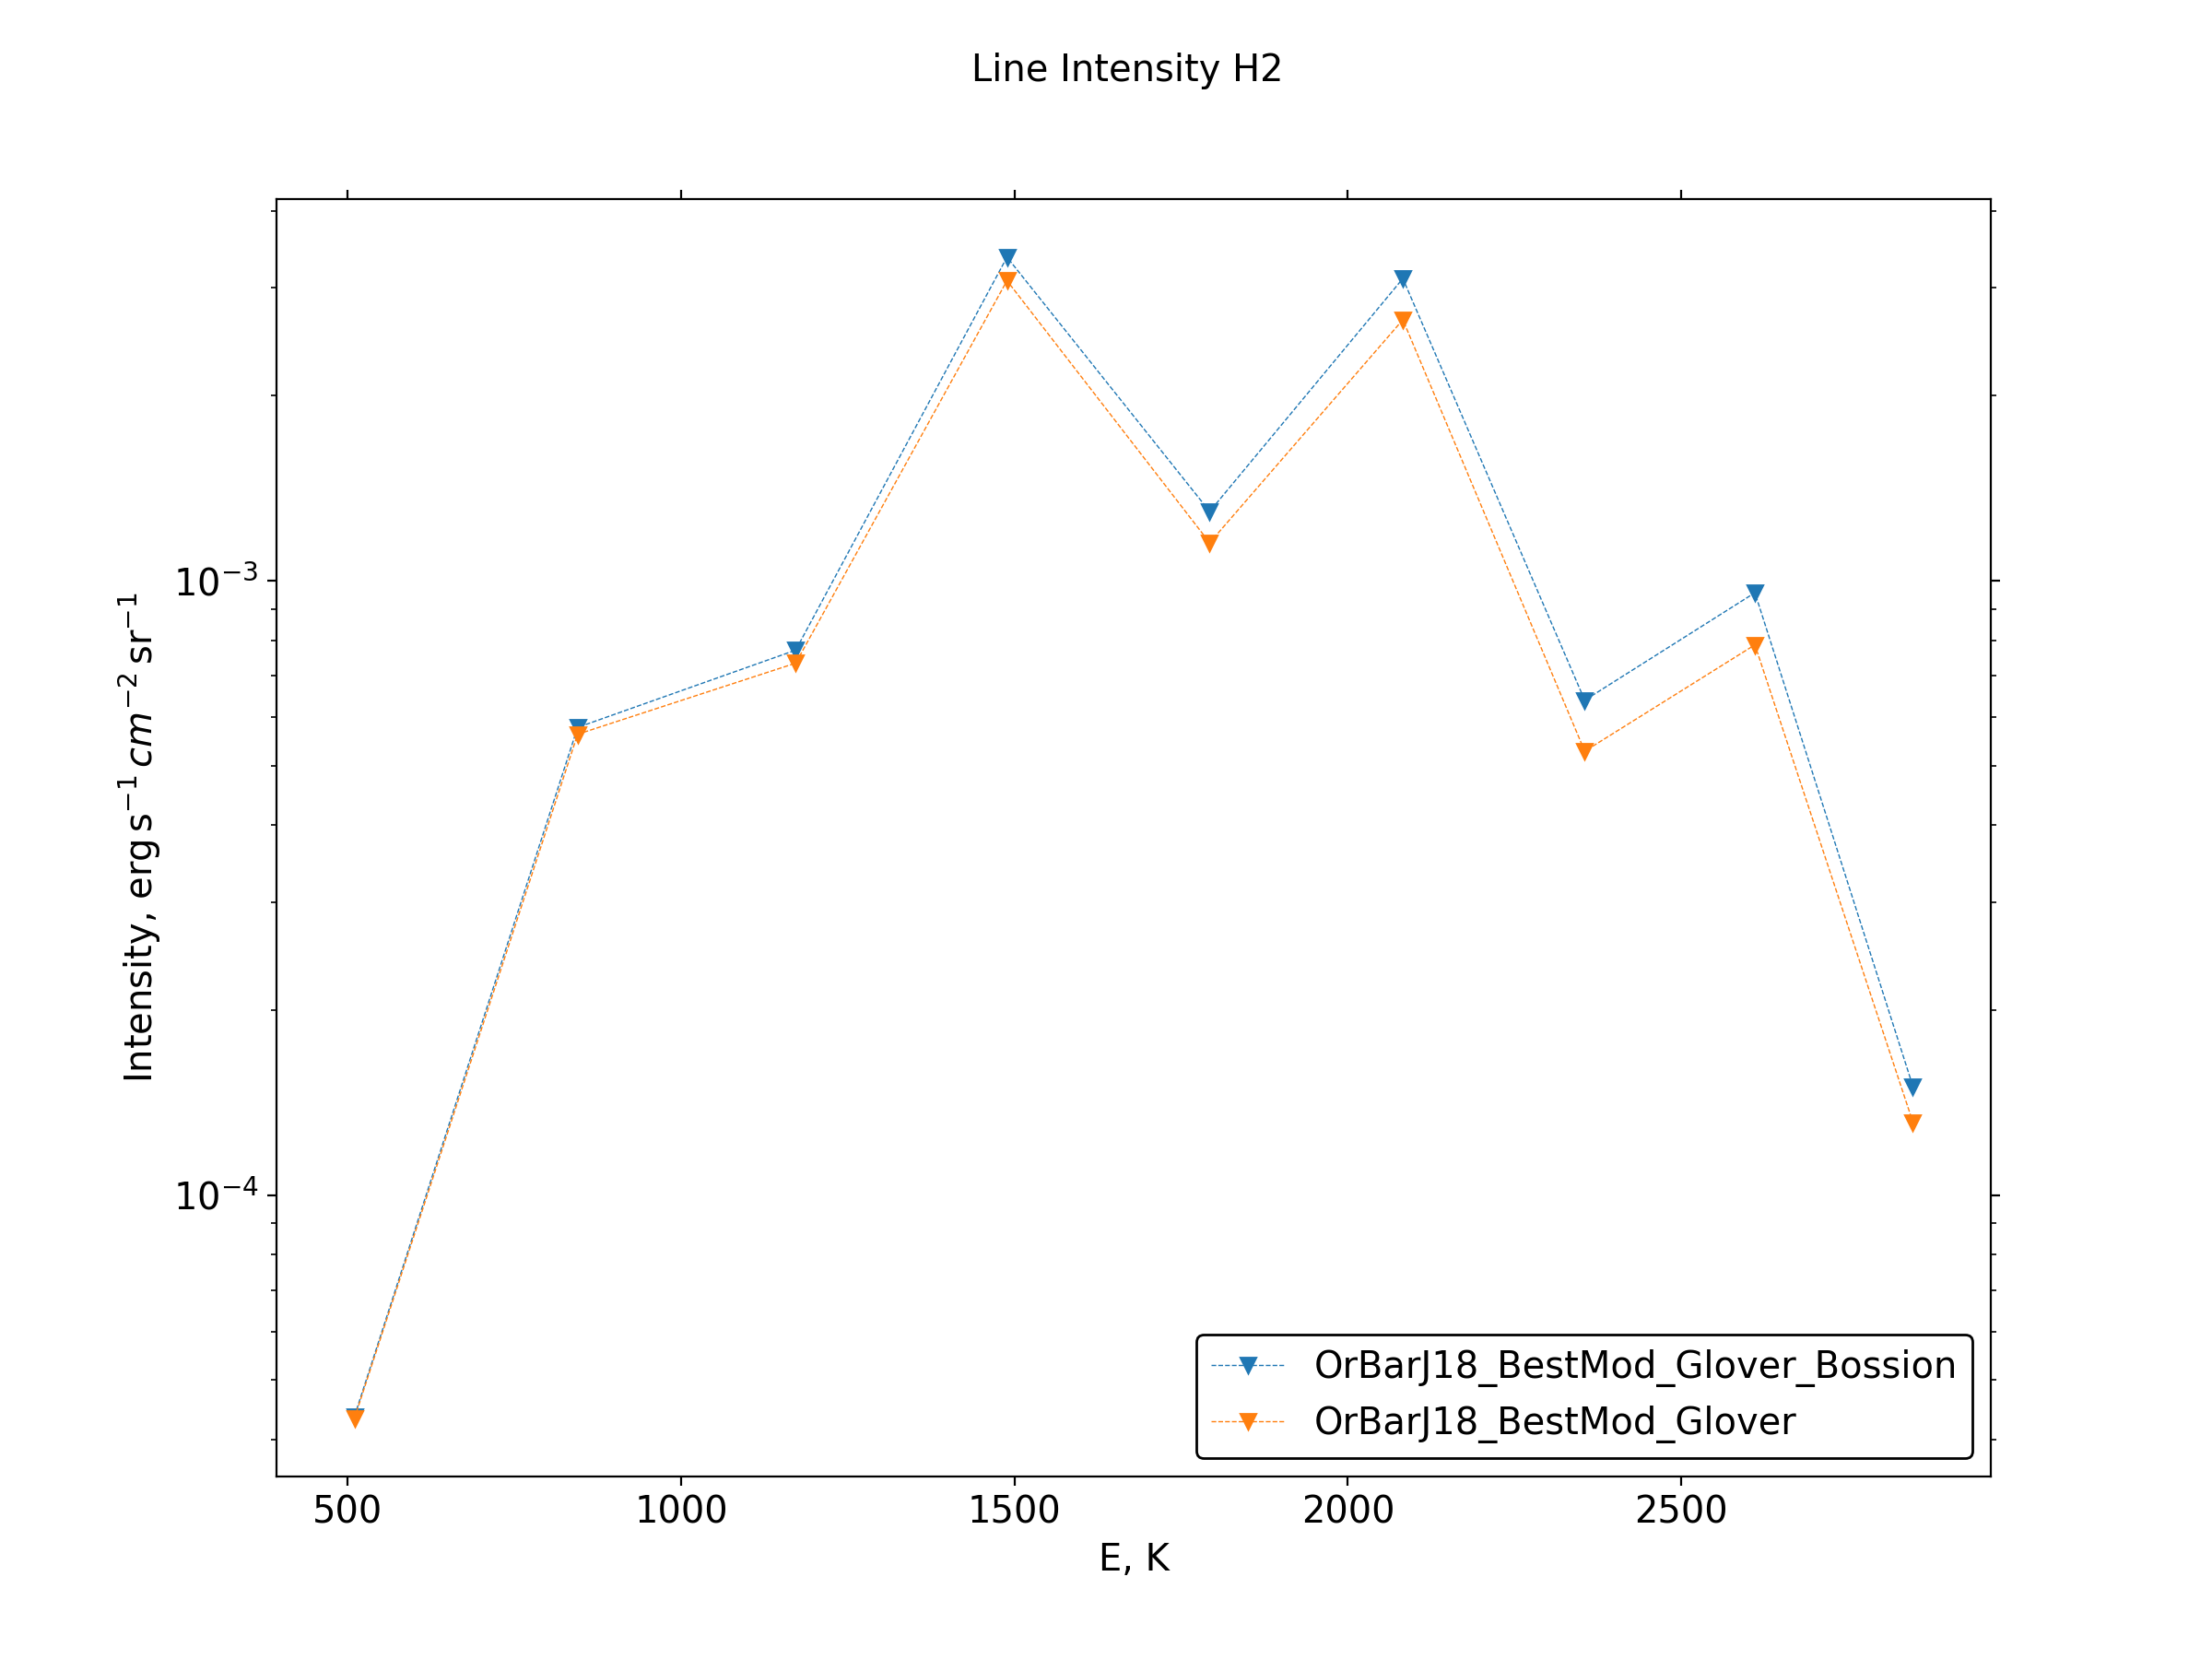
\includegraphics[trim = {0 0 0 1.5cm},clip,width=1\textwidth]{figure/H2/GloverBossion/I_comp_H2.png}
%         \caption{Spectre de $\mathrm{CO}$}
%     \end{subfigure}
%     ~ 
%     \begin{subfigure}[t]{0.49\textwidth}
%         \centering 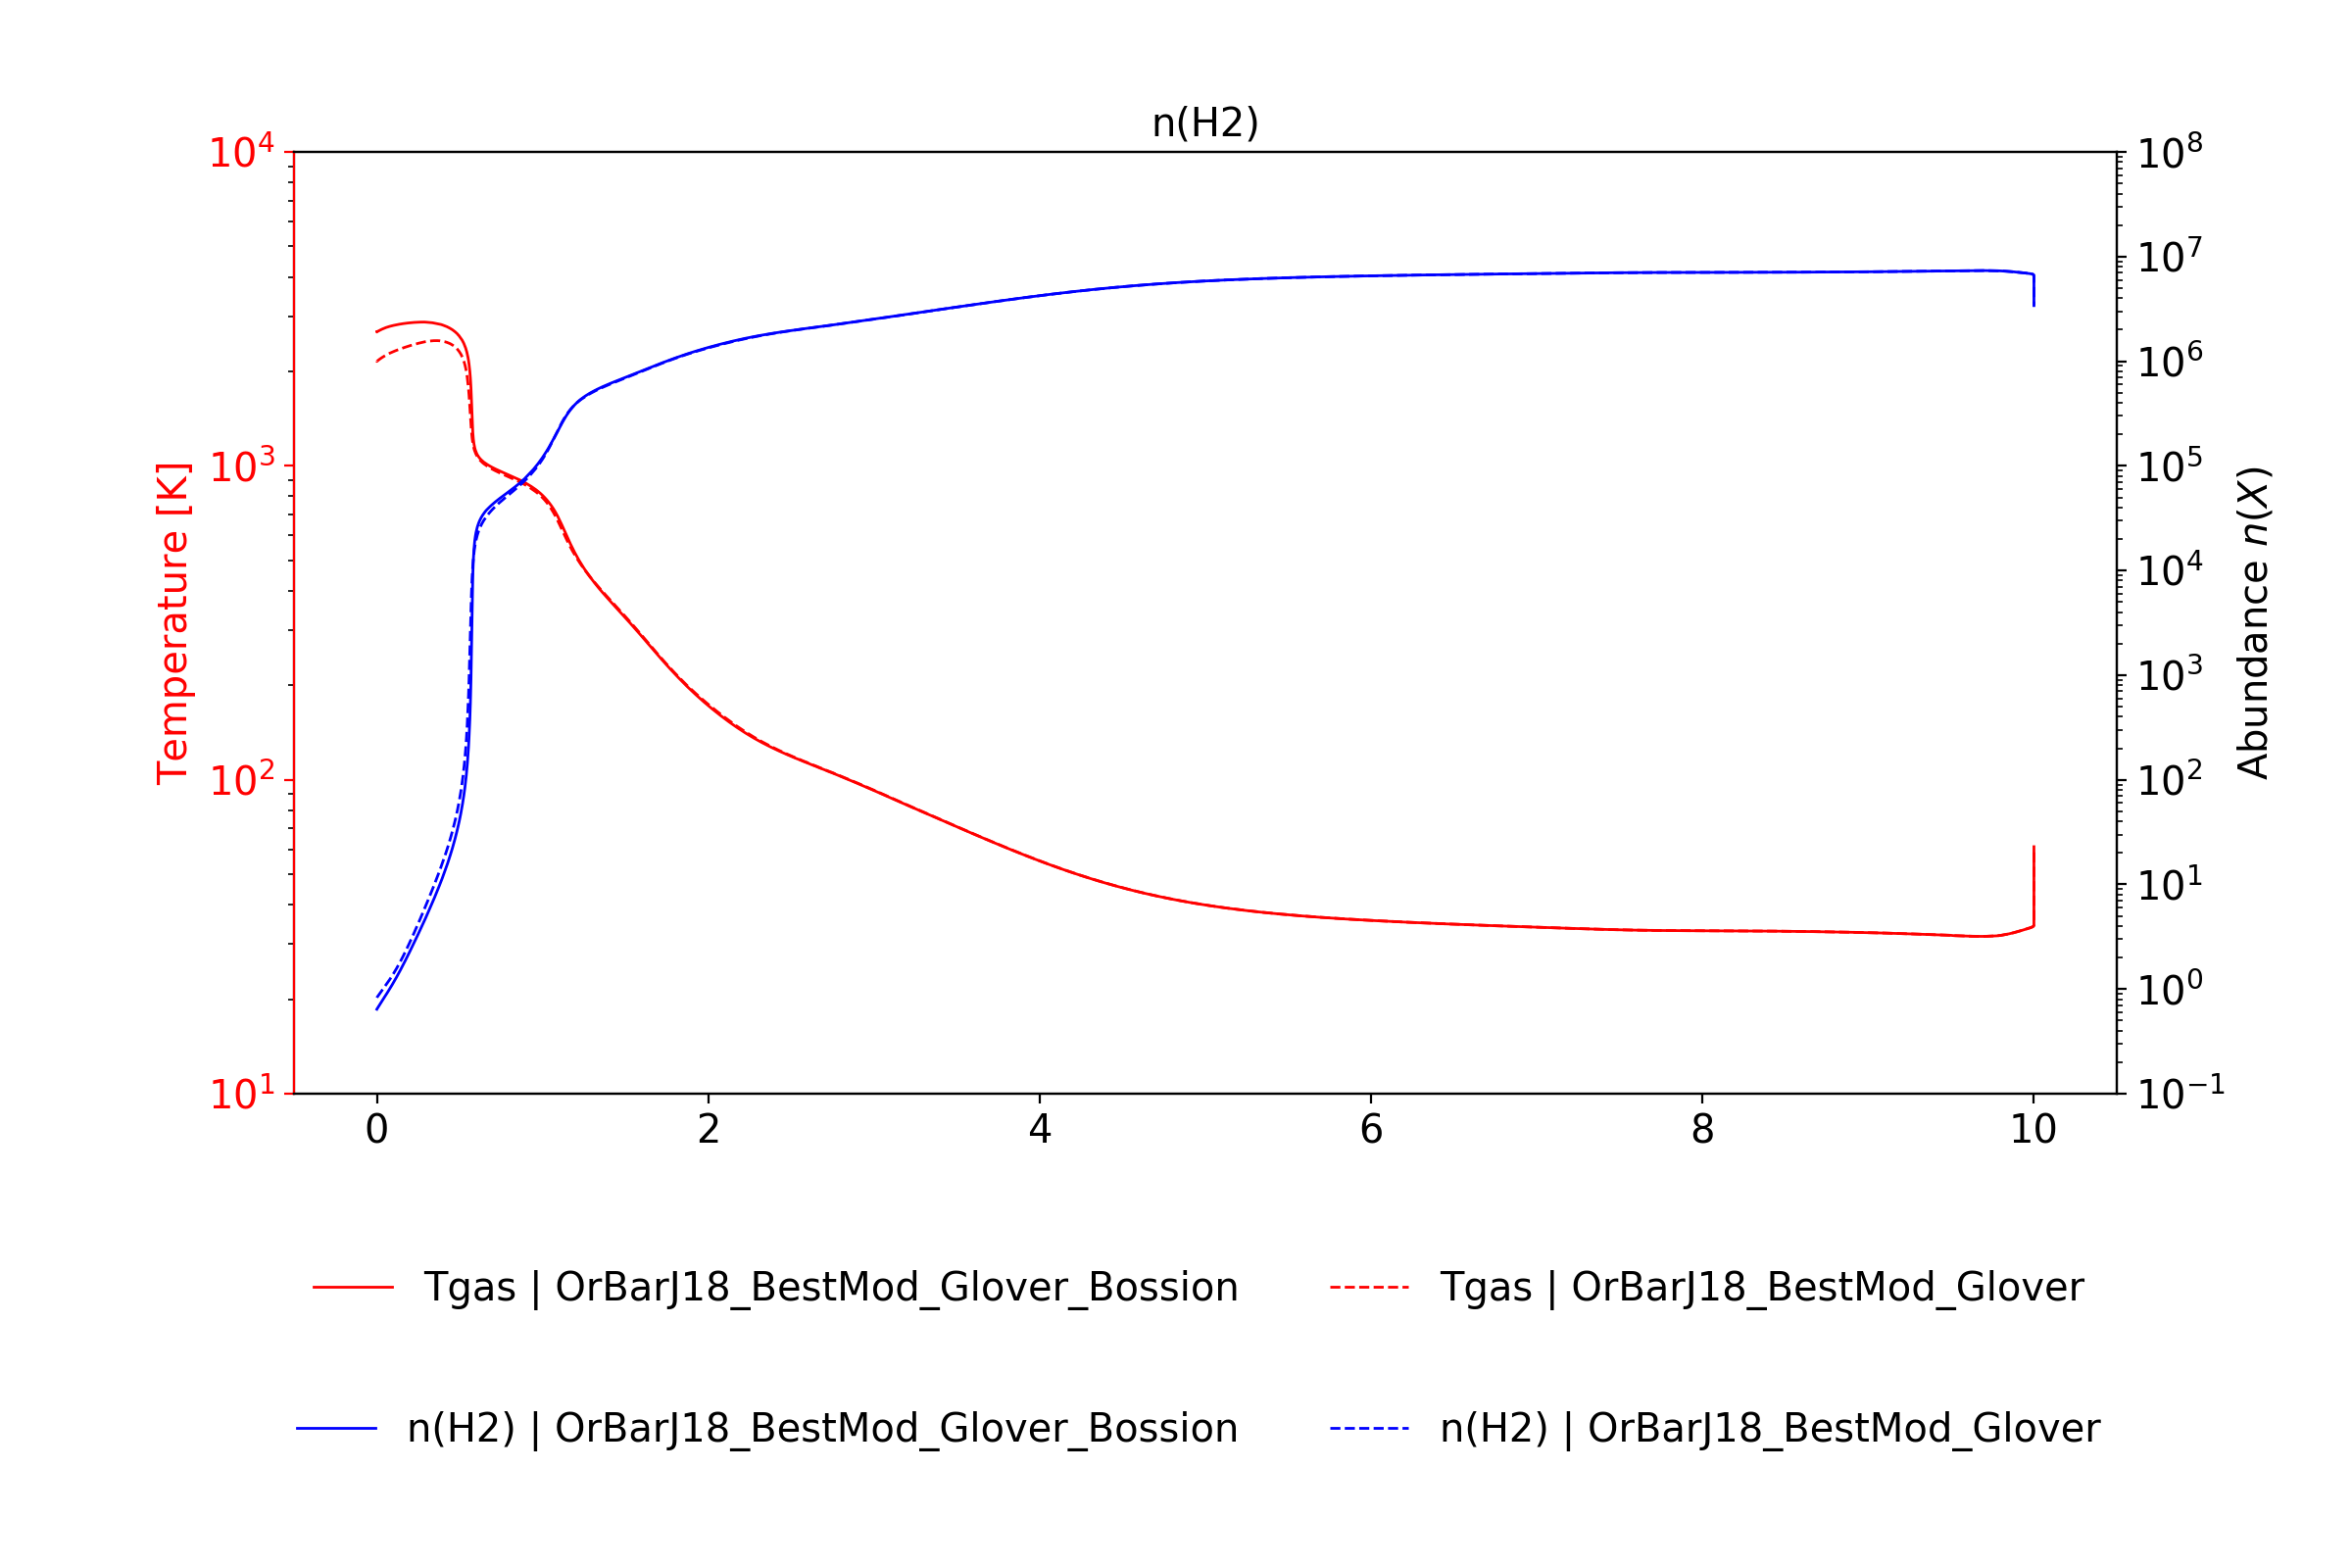
\includegraphics[trim = {0 0 0 1.5cm},clip,width=1\textwidth]{figure/H2/GloverBossion/nT_comp_H2.png}
%         \caption{Profil de densité et température de $\mathrm{CO}$}
%     \end{subfigure}
%     \caption{Comparaison des raies d'émissions des traceurs $\mathrm{H}_2$ et $\mathrm{CO}$ entre les calculs avec ou sans Bossion}
%     \label{fig:H2:GloverBossion:emiss}
% \end{figure}

% \subsection{Utilisation des nouveaux taux de collisions (Glover)}
% \subsection{A la recherche de l'instabilité par $\mathrm{H}_2$}
% \subsubsection{Où le chauffage par $\mathrm{H}_2$ prédomine-t-il dans le nuage ?}

% On a choisit quelques modèles parmi l'ensemble des calculs de la version \unsept utilisant les nouveaux taux de collisions. Il s'agit toujours de modèles à densités constantes. Ils sont symbolisé par des cercles pleins (en noirs) sur la figure \ref{fig:H2:mapGloverBossion:Gmax} et ont des conditions physiques différentes. On trace leurs profils de température à travers le nuage et l'on observe plusieurs choses (\autoref{fig:H2:mapGloverBossion:profilTx}) :  

% \begin{figure}[h!]
%     \centering
%     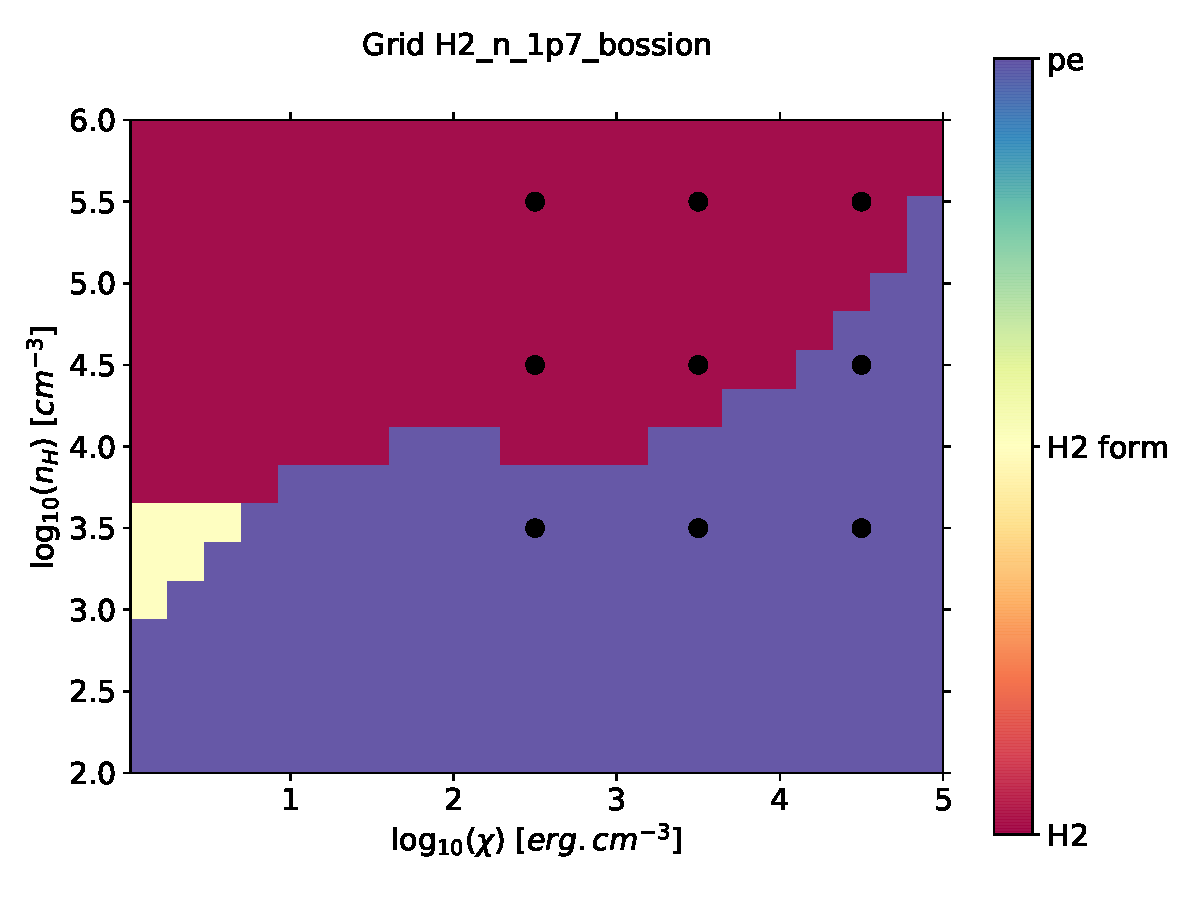
\includegraphics[width = 0.6\textwidth]{figure/H2/grid_gloverBossion/mapGmax_cross.pdf}
%     \caption{}
%     \label{fig:H2:mapGloverBossion:Gmax}
% \end{figure}


% \begin{itemize}
%     \item On voit (d) que la température au bord du nuage augmente pour les fort champs de rayonnement et que cette tendance est moins vraie (c) si le chauffage par $\mathrm{H}_2$ cesse de prédominer en bord de nuage (\ref{fig:H2:mapGloverBossion:Gmax}). Il vient un $\chi$ où la température augmente de manière raide à l'entrée du nuage moléculaire (a - $n_H = 10^{3.5}$ et $\chi = 10^{4.5}$). Je présume que c'est la recombinaison sur les grains qui est accélérée par le début de formation de $\mathrm{H}_2$ mais A VERIFIER. Comparer les $\Gamma$ et $\Lambda$ en fonction de la profondeur du nuage pour quelques modèles qui nous intéresse.
%     \item Si l'on se place à grand $\chi$ (b) le chauffage par $\mathrm{H}_2$ commence à prédominer en bord de nuage et on voit qu'il efface l'augmentation de température devant la partie moléculaire à mesure que le nuage devient dense. De même, en comparant (a) et (c), la recombinaison des grains s'intensifie avec le champs de rayonnement.
%     \item A forte densité (d) il apparaît un petit plateau après la transition $\mathrm{H}/\mathrm{H}_2$ : est ce que cela est du à l'effet photoélectrique ? pourrait il exciter d'avantage les raies du H2 ? On a vu avant qu'elle pouvait être du au chauffage par réactions chimiques qui devenait important car Glover tue la dissociation du H2. Et si l'on tracait ce T à cet endroit du nuage dans l'espace des paramètres. Peut être que l'on verrait aussi un bistabilité ? (première fois ou le gradient de T est minimale après la transition)
%     \item La température de la transition ne change pas d'un poil avec $\chi$ mais bouge avec la densité. Un fort champ de rayonnement ne fera que déplacer l'AV mais pas la température. Se comprend un peu car $\Gamma \propto n^2$ et $\Lambda \propto n $ mais pas toujours $\propto \chi$.
% \end{itemize}

% \begin{figure}[h!]
%     \centering
%     \begin{subfigure}[t]{0.49\textwidth} % "0.49" donne ici la largeur de l'image
%         \centering 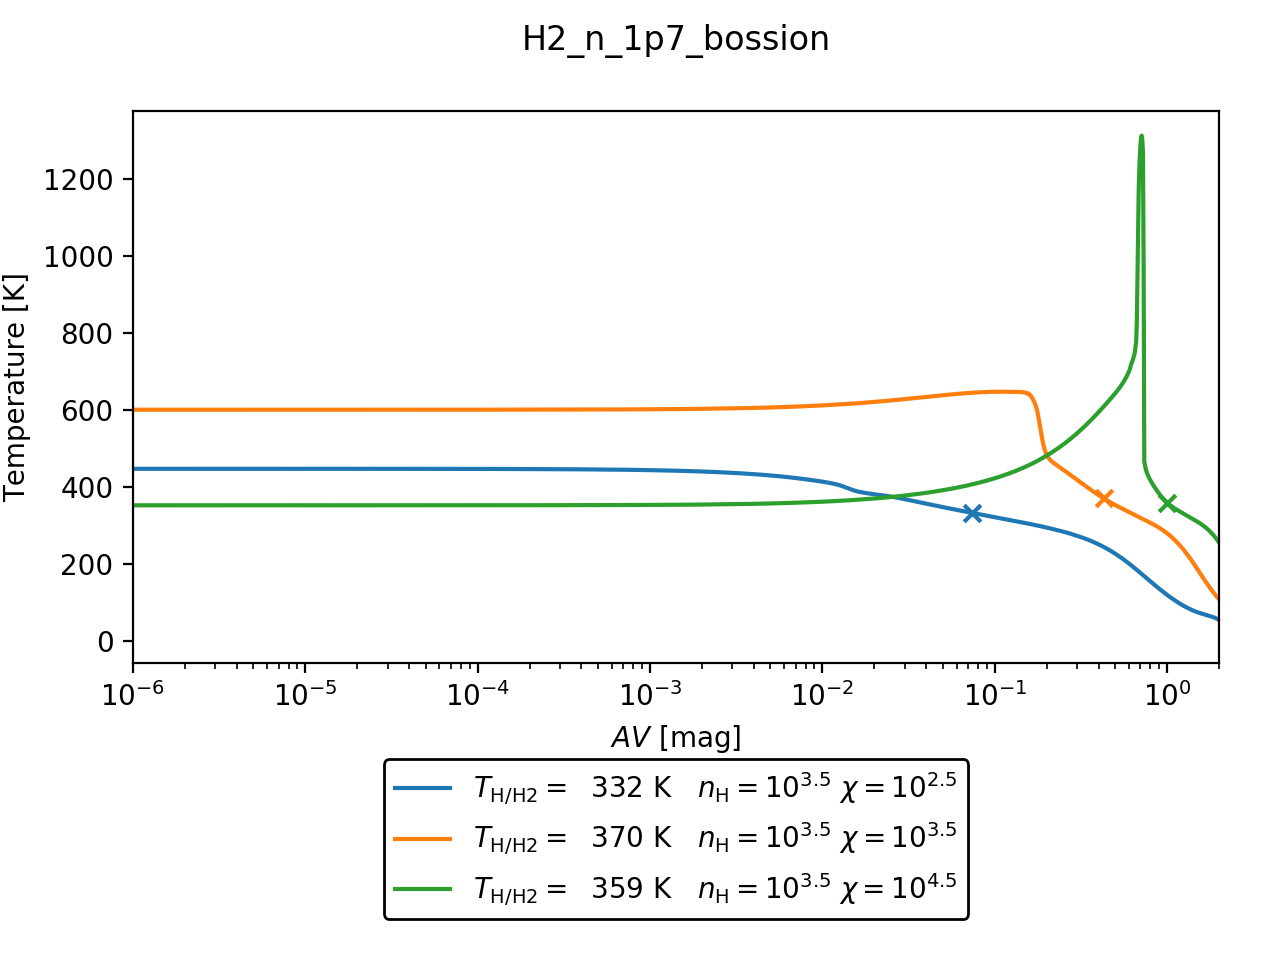
\includegraphics[trim = {0 0 0 0},clip,width=1\textwidth]{figure/H2/grid_gloverBossion/H2_n_1p7_bossion_d3p5r2p5_d3p5r3p5_d3p5r4p5.png} 
%         \caption{}
%     \end{subfigure}
%     ~ 
%     \begin{subfigure}[t]{0.49\textwidth}
%         \centering 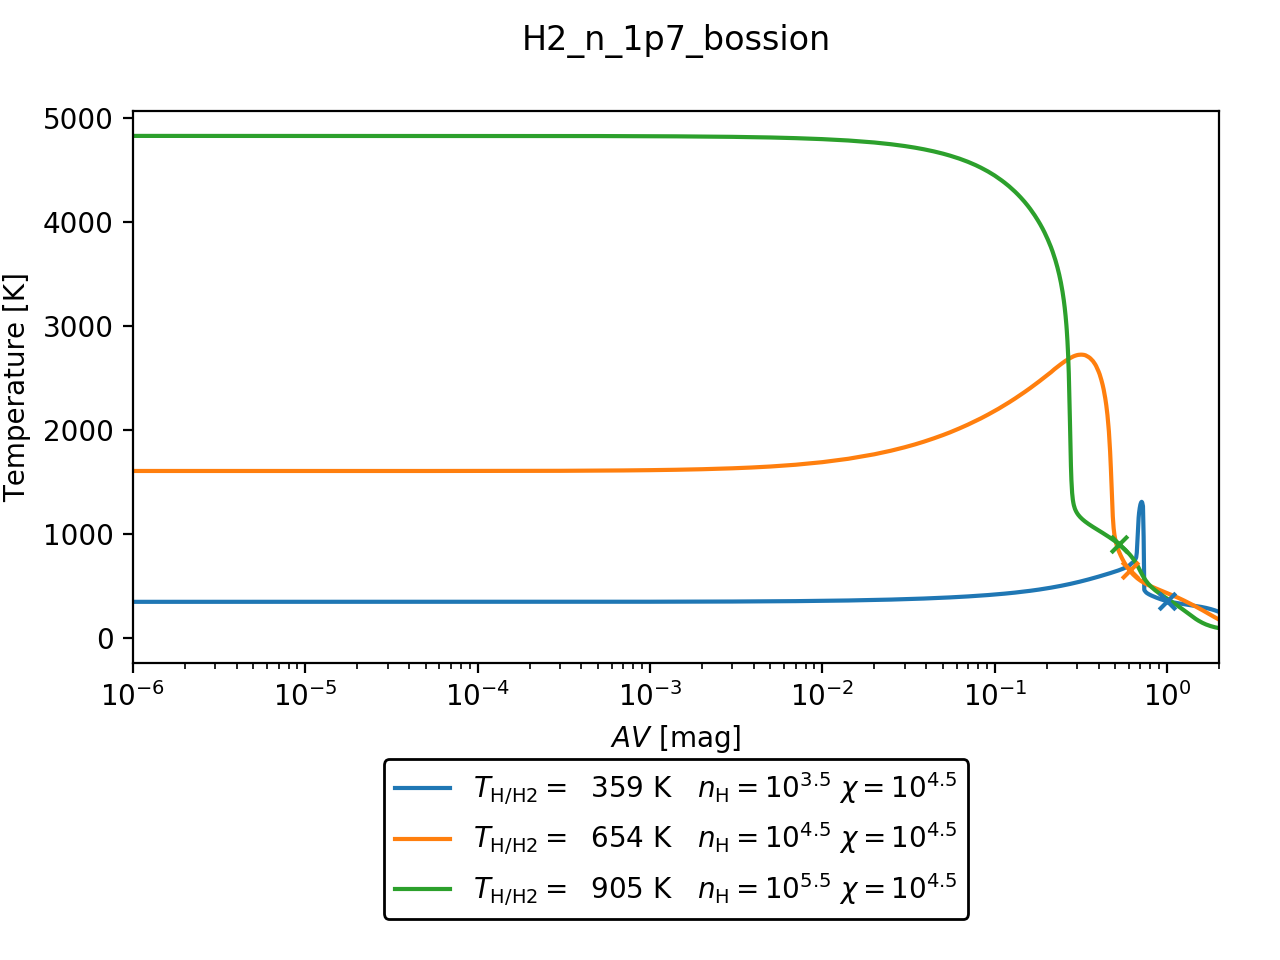
\includegraphics[trim = {0 0 0 0},clip,width=1\textwidth]{figure/H2/grid_gloverBossion/H2_n_1p7_bossion_d3p5r4p5_d4p5r4p5_d5p5r4p5.png}
%         \caption{}
%     \end{subfigure}

%     \centering
%     \begin{subfigure}[t]{0.49\textwidth} % "0.49" donne ici la largeur de l'image
%         \centering 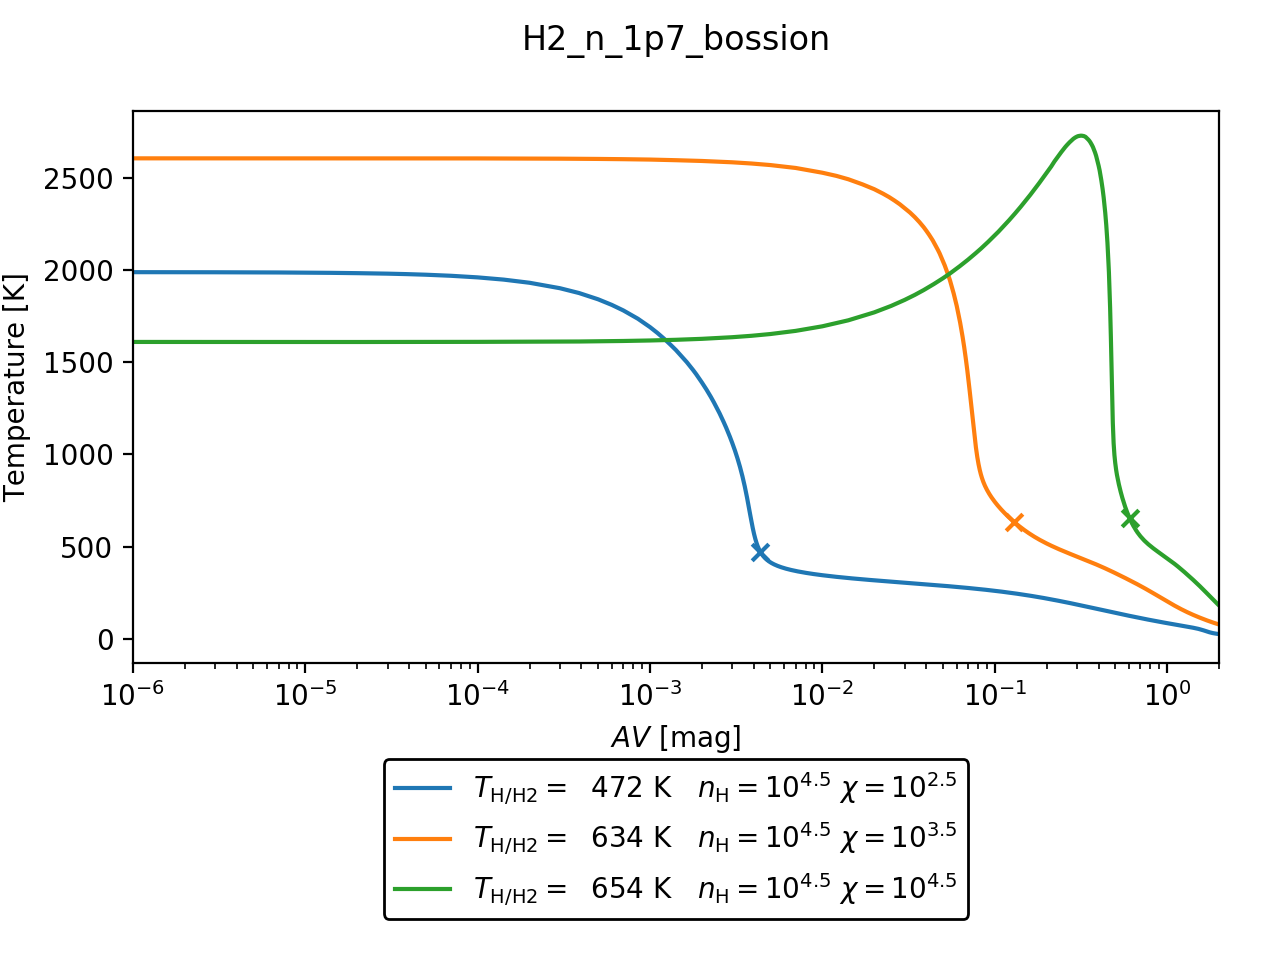
\includegraphics[trim = {0 0 0 0},clip,width=1\textwidth]{figure/H2/grid_gloverBossion/H2_n_1p7_bossion_d4p5r2p5_d4p5r3p5_d4p5r4p5.png} 
%         \caption{}
%     \end{subfigure}
%     ~ 
%     \begin{subfigure}[t]{0.49\textwidth}
%         \centering 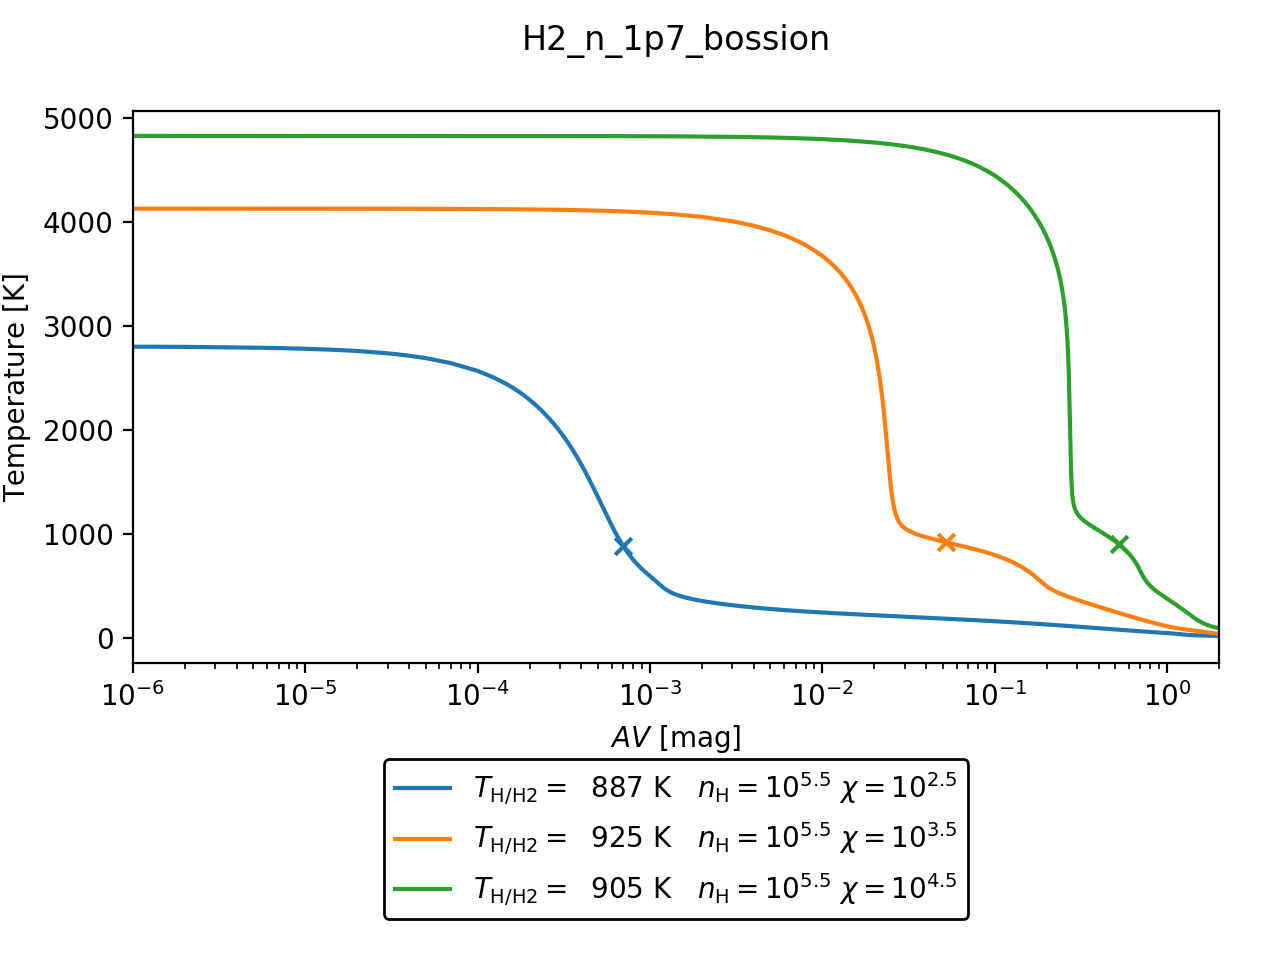
\includegraphics[trim = {0 0 0 0},clip,width=1\textwidth]{figure/H2/grid_gloverBossion/H2_n_1p7_bossion_d5p5r2p5_d5p5r3p5_d5p5r4p5.png} 
%         \caption{}
%     \end{subfigure}
%     \caption{Profil de températures pour différent modèles de la grille (Glover + Bossion). La croix indique la température de la transition $\mathrm{H}/\mathrm{H}_2$ : $n(\mathrm{H})=2n(\mathrm{H}_2)$.}
%     \label{fig:H2:mapGloverBossion:profilTx}
% \end{figure}

% \subsection{Dans quelles conditions le chauffage par $\mathrm{H}_2$ prédomine-t-il ?}

% On observe également la température de la transition $\mathrm{H}/\mathrm{H}_2$ dans l'espace des paramètres (\autoref{fig:H2:mapGloverBossion:mapTHH2}). La température ne dépend toujours pas de l'intensité du champs de rayonnements et on arrive encore à dépasser le plateau de $600K$. Cependant les nouveaux taux de collisions n'apportent rien.\newline 

% \begin{figure}[th!]
%     \centering
%     \begin{subfigure}[t]{0.49\textwidth} % "0.49" donne ici la largeur de l'image
%         \centering 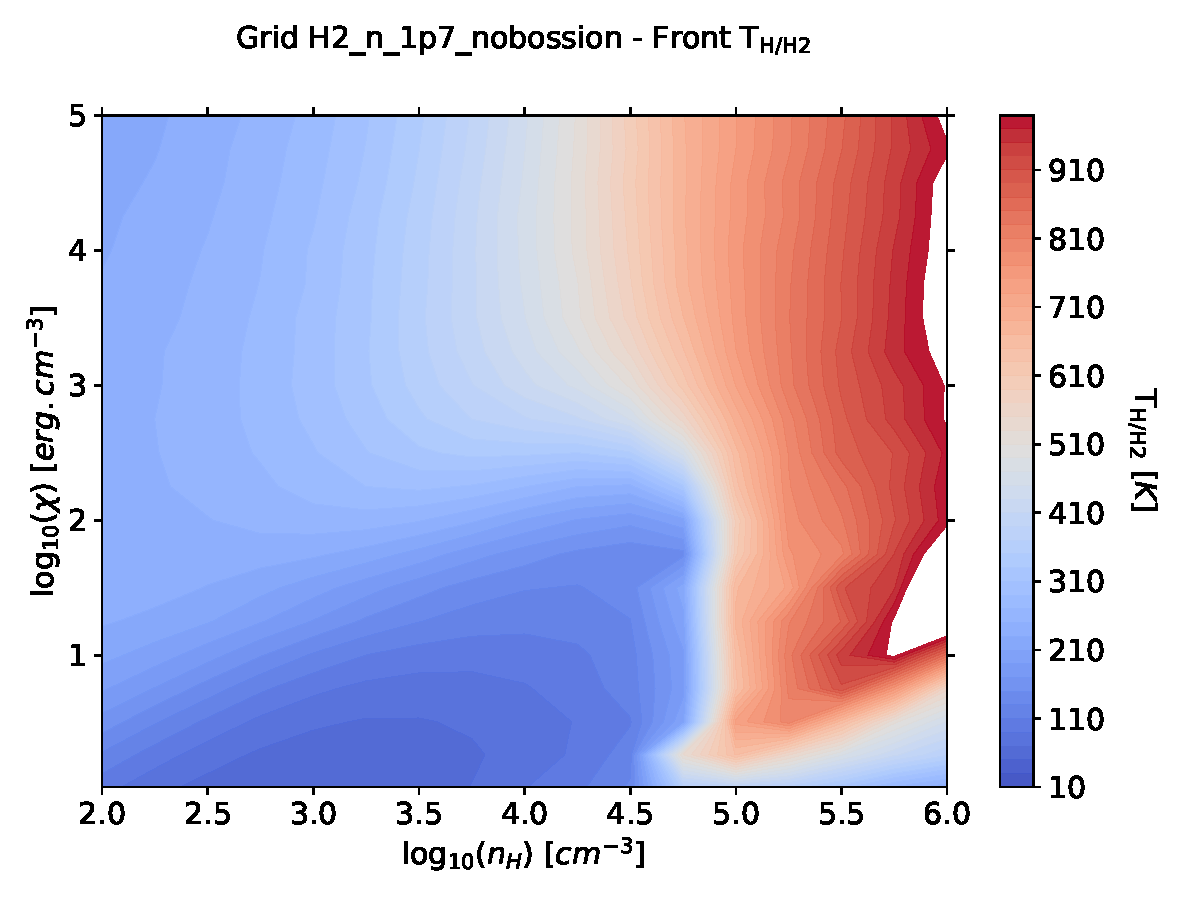
\includegraphics[trim = {0 0 0 0},clip,width=1\textwidth]{figure/H2/grid_glovernoBossion/HH2_T_Franck.pdf}
%         \caption{}
%     \end{subfigure}
%     ~ 
%     \begin{subfigure}[t]{0.49\textwidth}
%         \centering 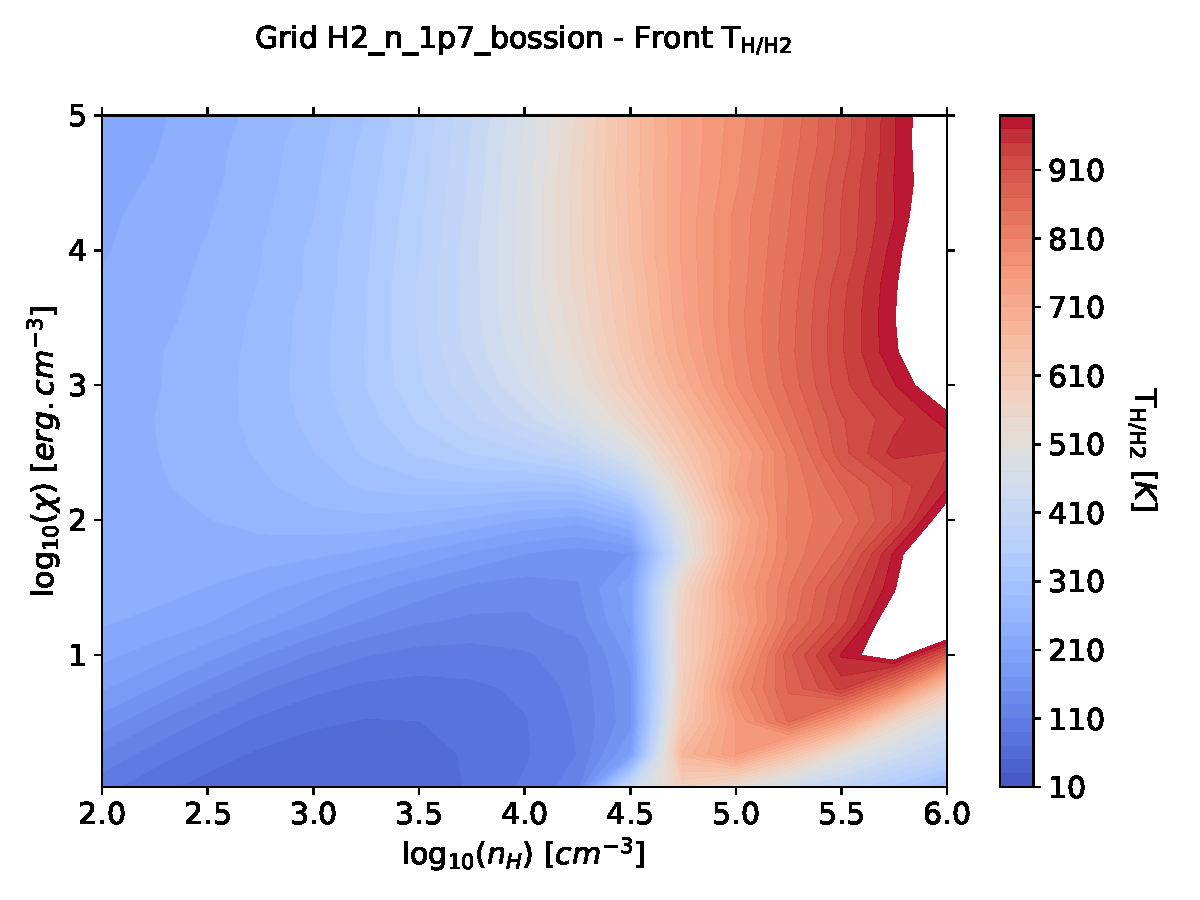
\includegraphics[trim = {0 0 0 0},clip,width=1\textwidth]{figure/H2/grid_gloverBossion/HH2_T_Franck.pdf}
%         \caption{}
%     \end{subfigure}
%     \caption{Carte de températures de la transition $\mathrm{H}/\mathrm{H}_2$ : $n(\mathrm{H})=2n(\mathrm{H}_2)$ avec (a) ou sans (b) les niveaux de Bossion (Glover)}
%     \label{fig:H2:mapGloverBossion:mapTHH2}
% \end{figure}

% \underline{Conclusion partielle :}On voit que le chauffage par $\mathrm{H}_2$ concerne les régions denses et impactent principalement les bords atomiques. Or c'est si l'on chauffait l'entrée du nuage que l'on pourrait espérer observer les changements. Il faudrait regarder les diagrammes d'excitations de quelques espèces comme $\mathrm{H}_2$ ou $\mathrm{CO}$. On se pose également une question sur l'impact de la raideur de la transition sur la température (\autoref{fig:H2:mapGloverBossion:smooth}) : dans certains cas, la transition se fait pour des gaz encore chaud ce qui signifie que l'on pourrait voir des raies plus excitées. Dans quelles conditions ces phénomènes ont ils lieux ? Est ce que cela a un impact sur les raies ? 
% (Sternberg 2014) Enfin on n'a pas observé les instabilités que pouvait provoquer le $\mathrm{H}_2$. Tracer quelques courbes de chauffages et refroidissements pour différent modèles (là le gradient de Tmax) est maximale par exemple. On observait également mieux l'instabilité sur des modèles isobares : faire une petite grille. 
% Pour avancer sur cette histoire de chauffage par réaction chimiqie : tracer $\max_{AV} \Gamma_{ch}/\Gamma_{tot}$ dans l'espace des paramètres et le $(argmax_{AV}  \Gamma_{ch}/\Gamma_{tot})/AV_{HH2}$ qui est lié également au $\mathrm{H}_2$ par la réaction avec le $\mathrm{CH}^+$

% \begin{figure}[th!]
%         \centering 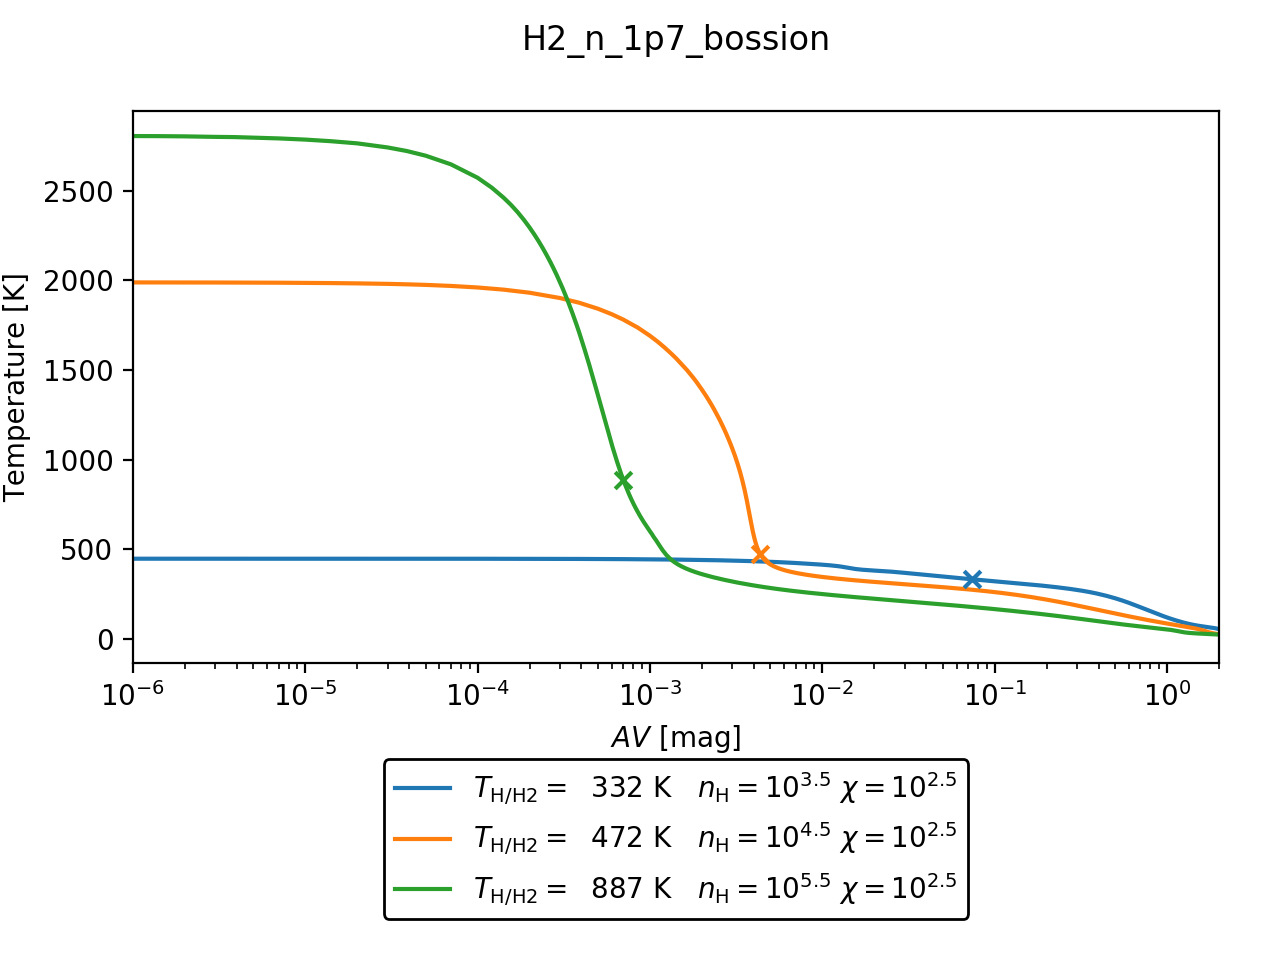
\includegraphics[trim = {0 0 0 0},clip,width=0.5\textwidth]{figure/H2/grid_gloverBossion/H2_n_1p7_bossion_d3p5r2p5_d4p5r2p5_d5p5r2p5.png}
%         \caption{Profils de températures de différents modèles de la grille (Glover + Bossion)}
%         \label{fig:H2:mapGloverBossion:smooth}
% \end{figure}

% \subsubsection{Dans quelles conditions peut on voir une instabilité ?}
% \subsubsection{Quel est l'impact sur les raies des traceurs ?}


% \subsubsection{Bonus}